\section{Control Plots for 2012A and 2012B}
\label{sec:CP2012AB}

In this chappter are presented the MC vs data plots for 2012A and 201B run period separately. 2012A period comprises run range 
[190456,193686] and 2012B - run range [193752,195552]. 

\begin{figure}[htb]
  \centering
    \subfigure[2012A: leading jet $p_{T}$]{
      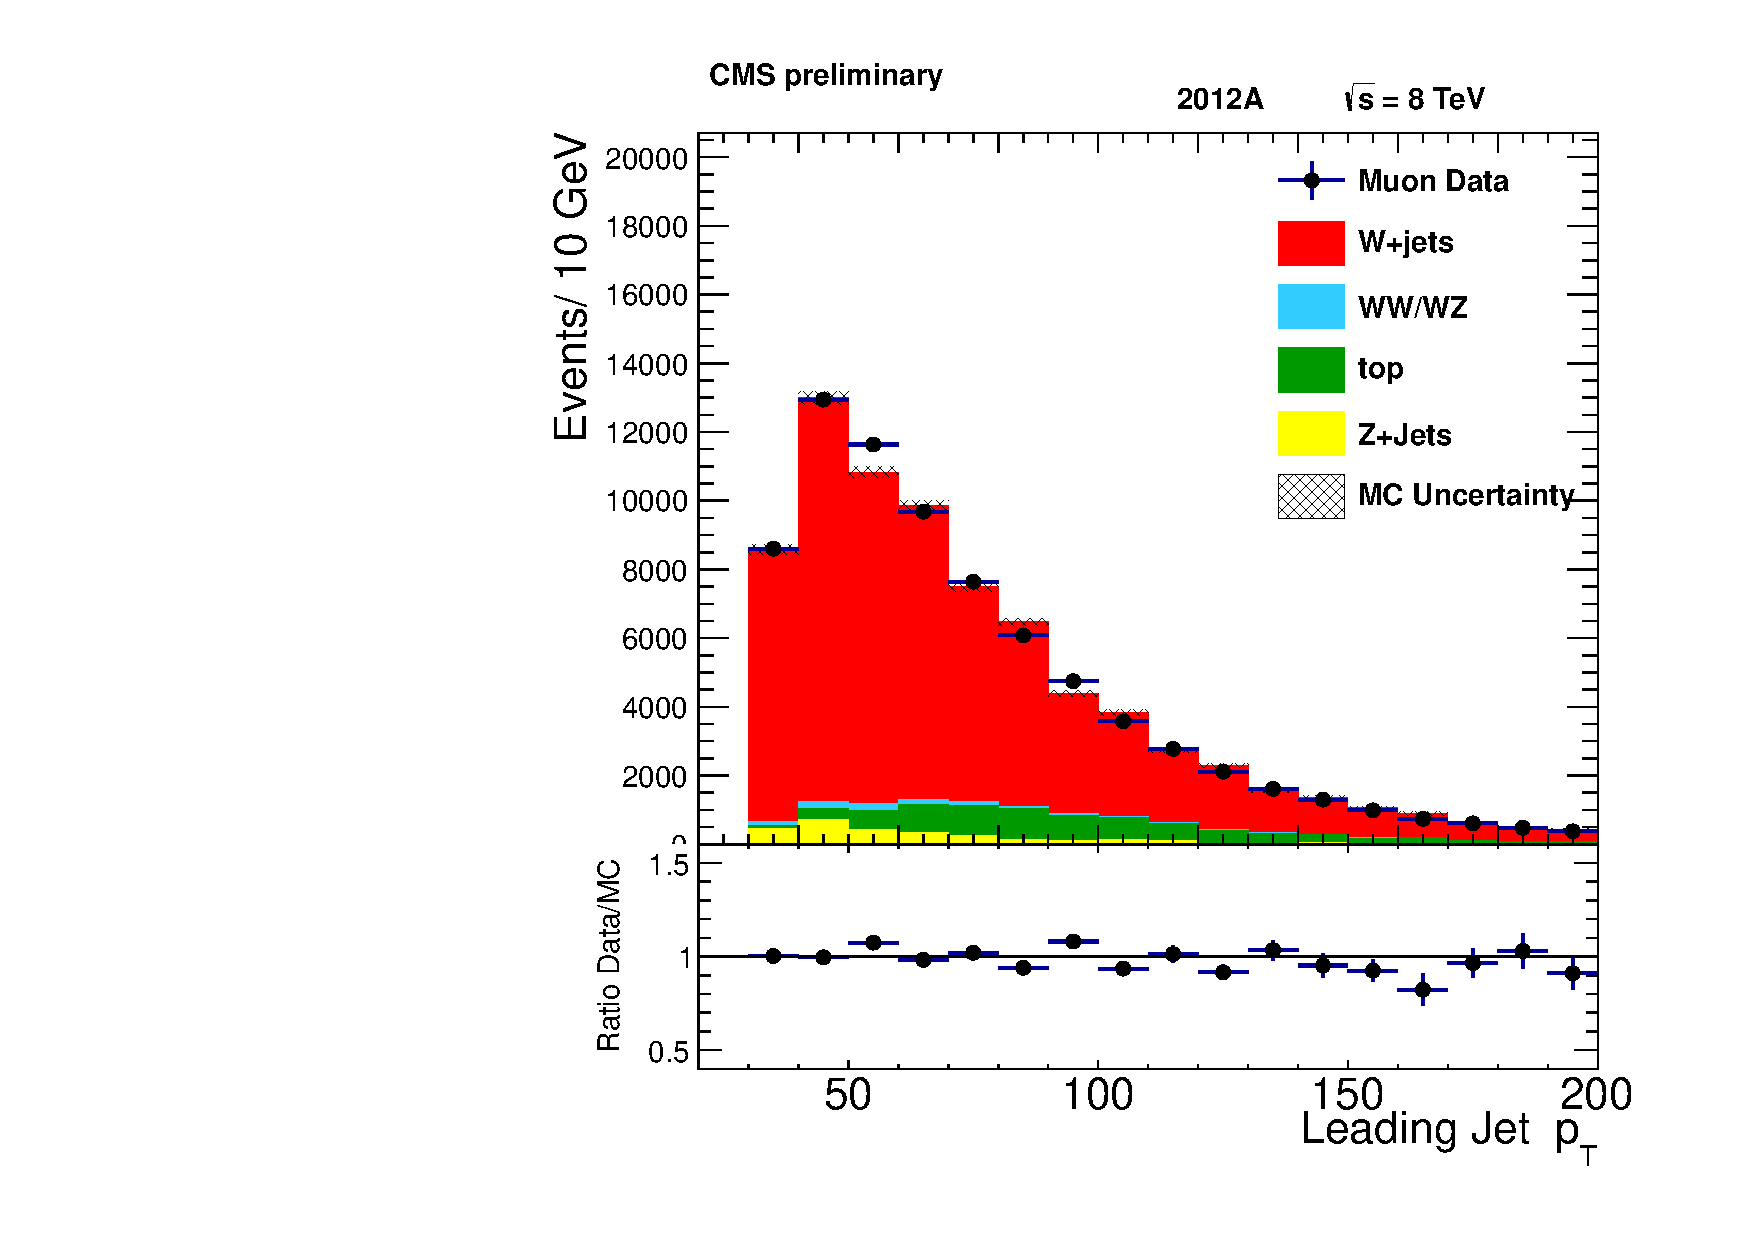
\includegraphics[width=0.3\textwidth]{plots/mu_jetld_pt_2012A.pdf}
    }
    \subfigure[2012B:  leading jet $p_{T}$]{
      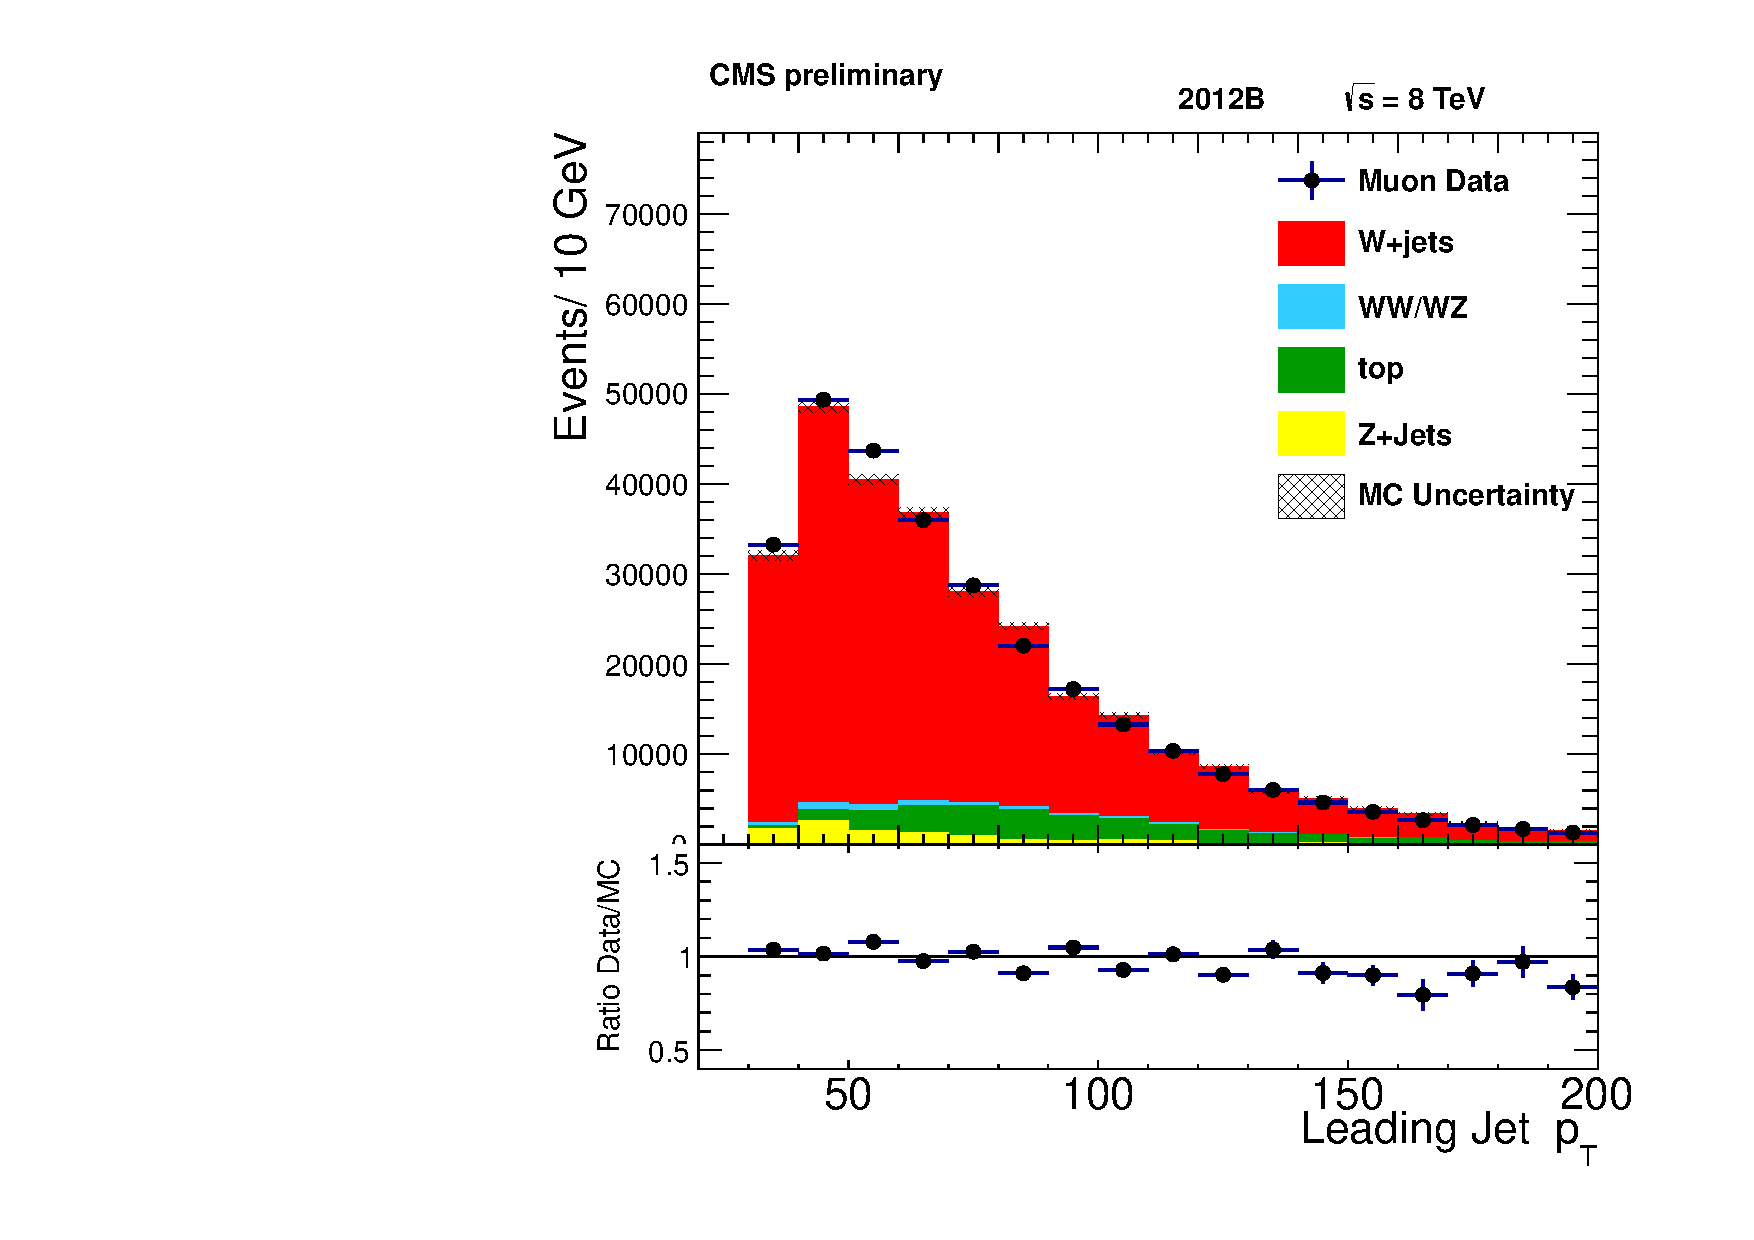
\includegraphics[width=0.3\textwidth]{plots/mu_jetld_pt_2012B.pdf}
    }
    \\
    \subfigure[2012A: second jet $p_{T}$]{
      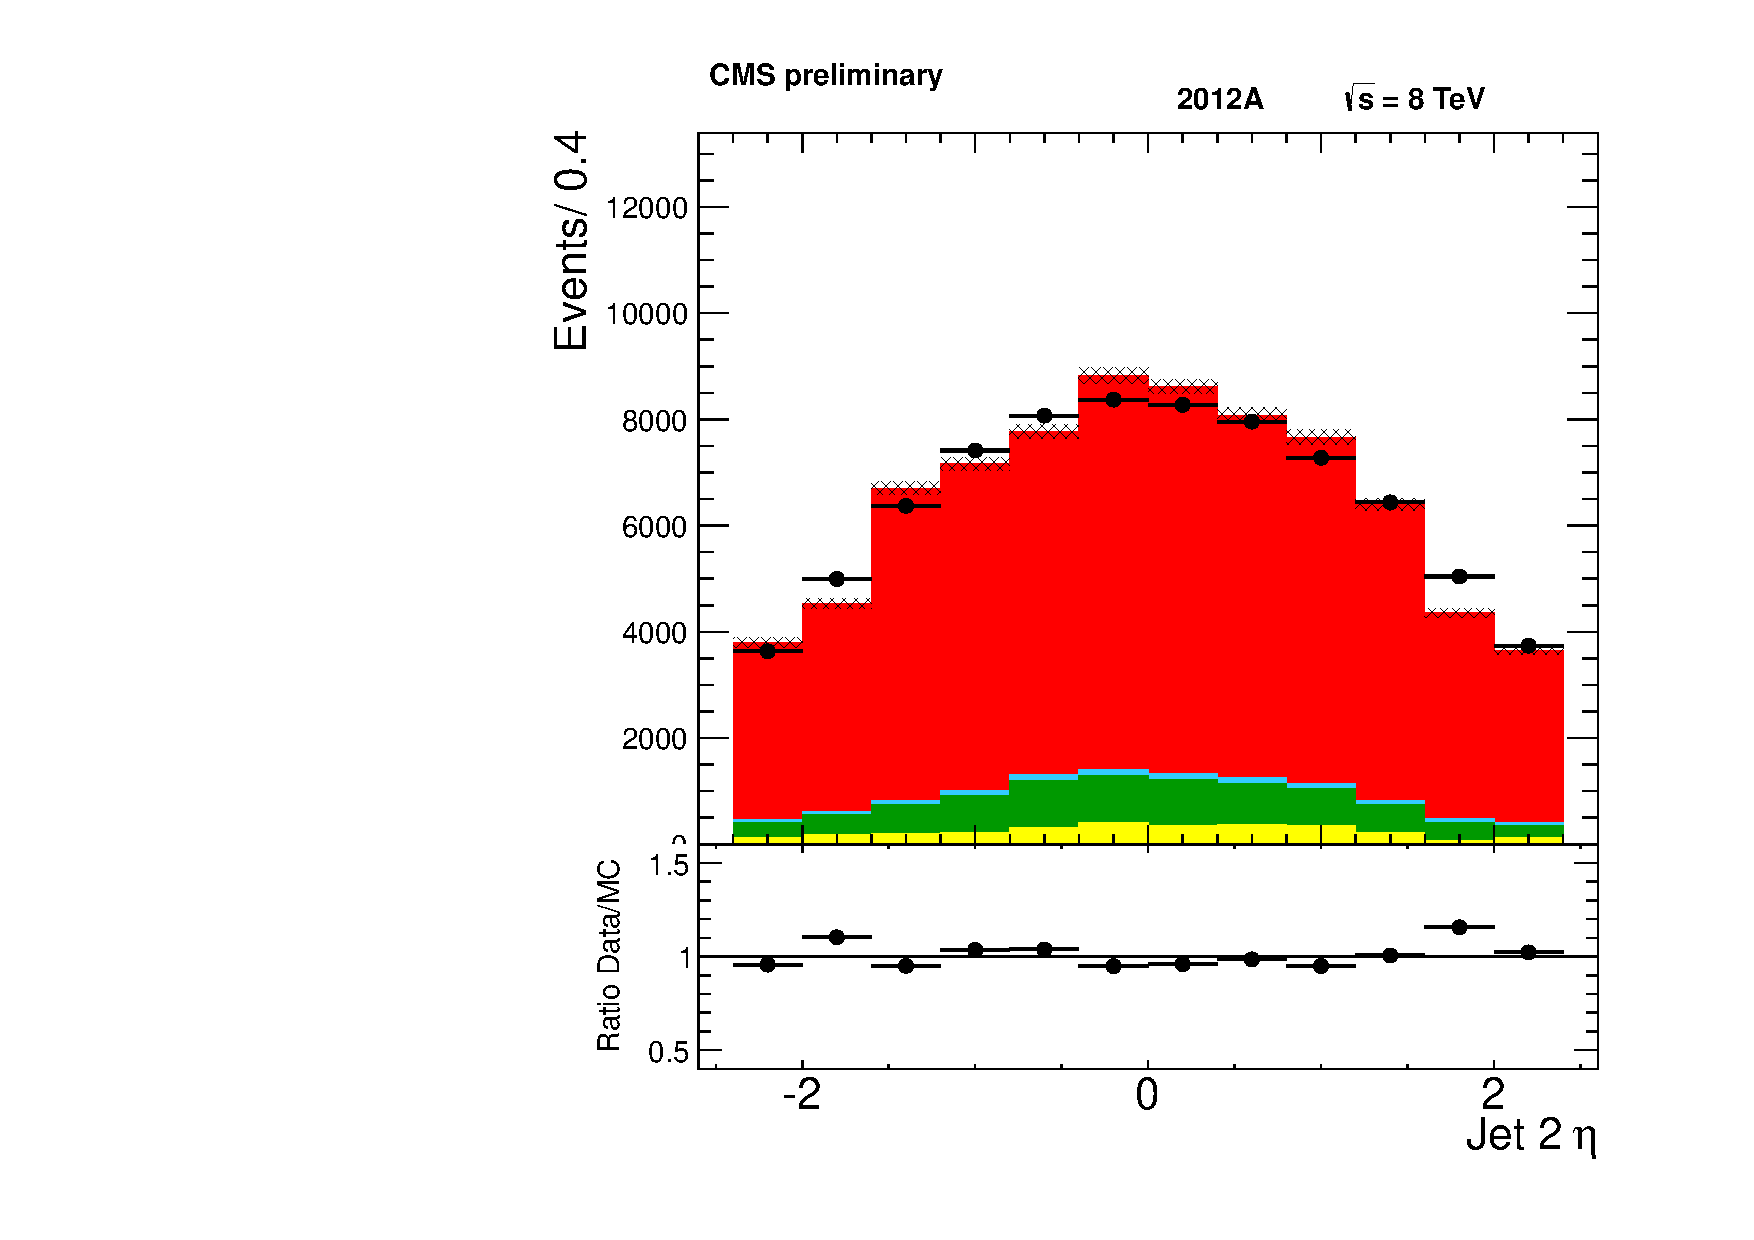
\includegraphics[width=0.3\textwidth]{plots/mu_jetnt_eta_2012A.pdf}
    }
    \subfigure[2012B: second jet $p_{T}$]{
      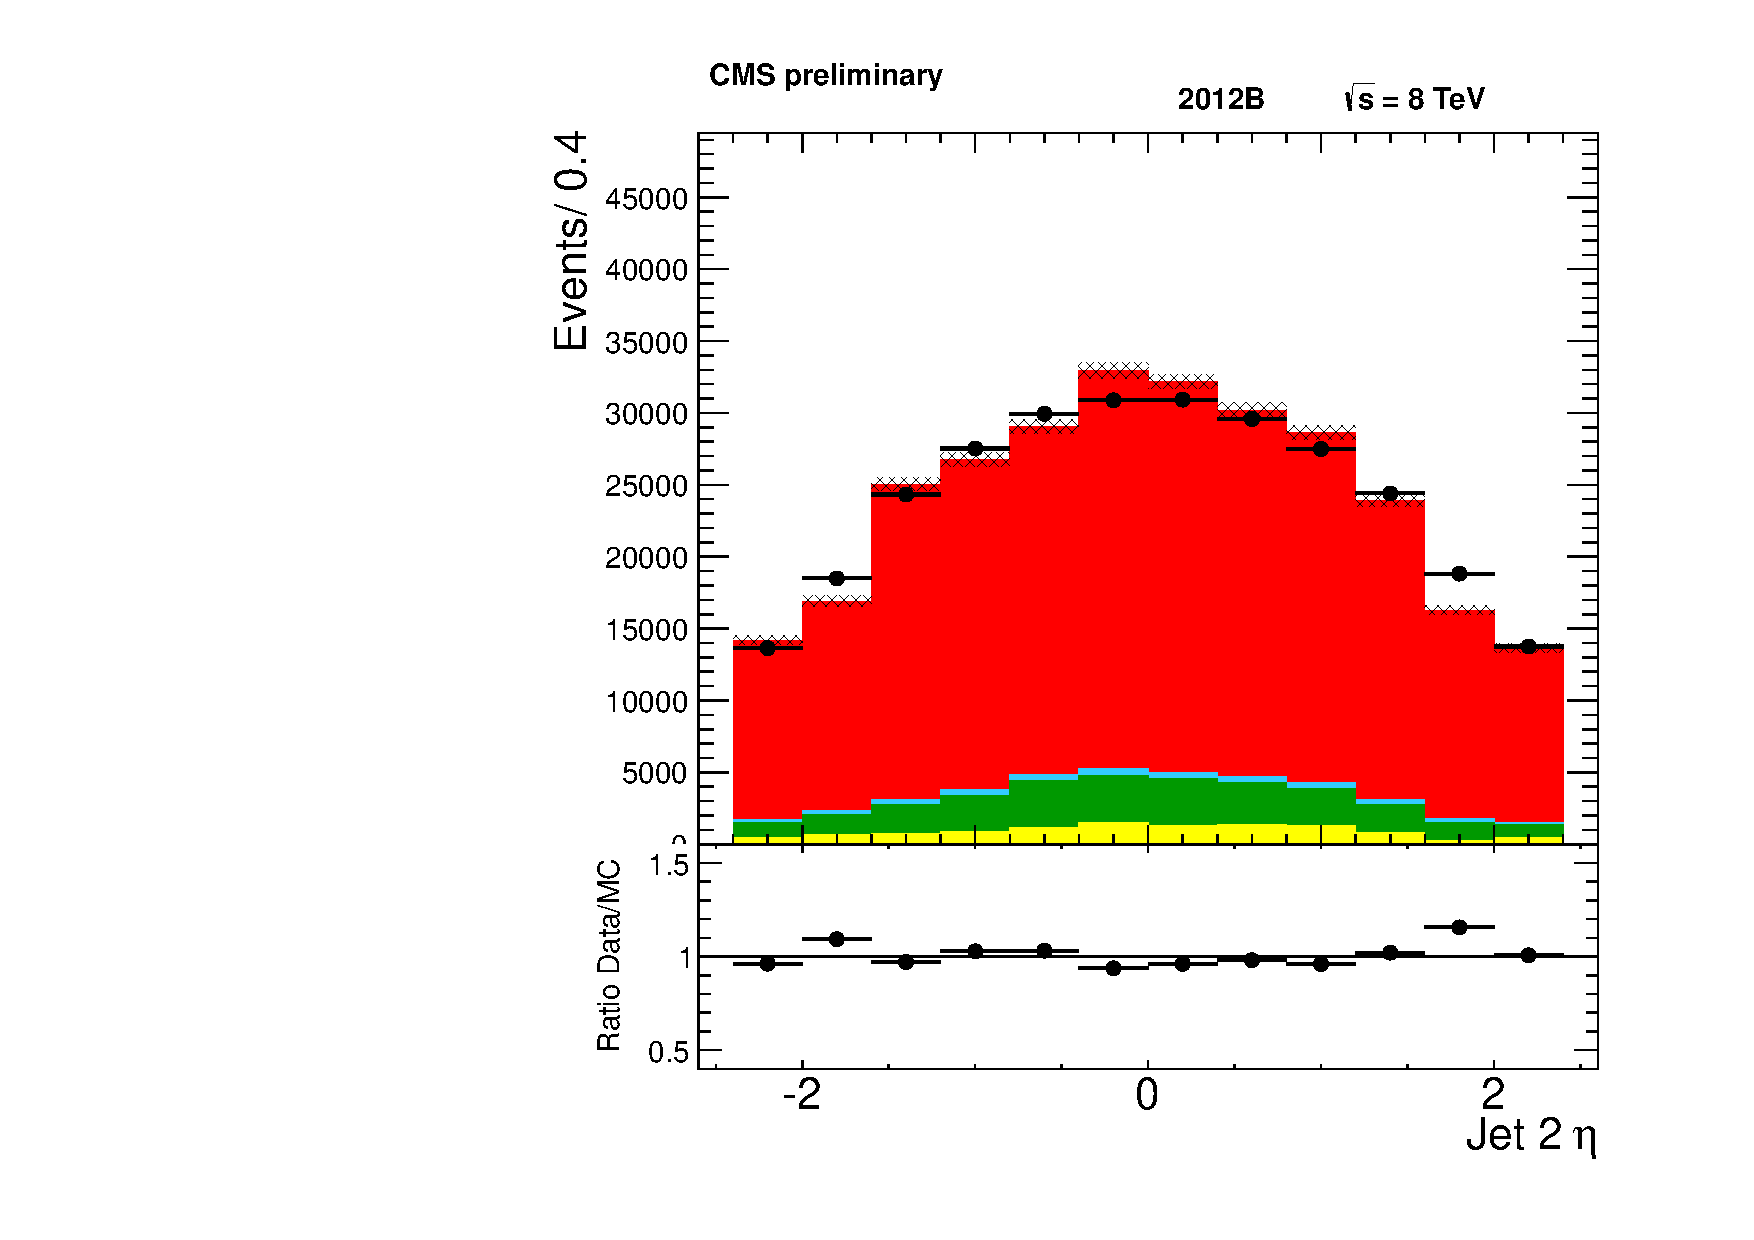
\includegraphics[width=0.3\textwidth]{plots/mu_jetnt_eta_2012B.pdf}
    }
    \\
    \subfigure[2012A: leading jet $\eta$]{
      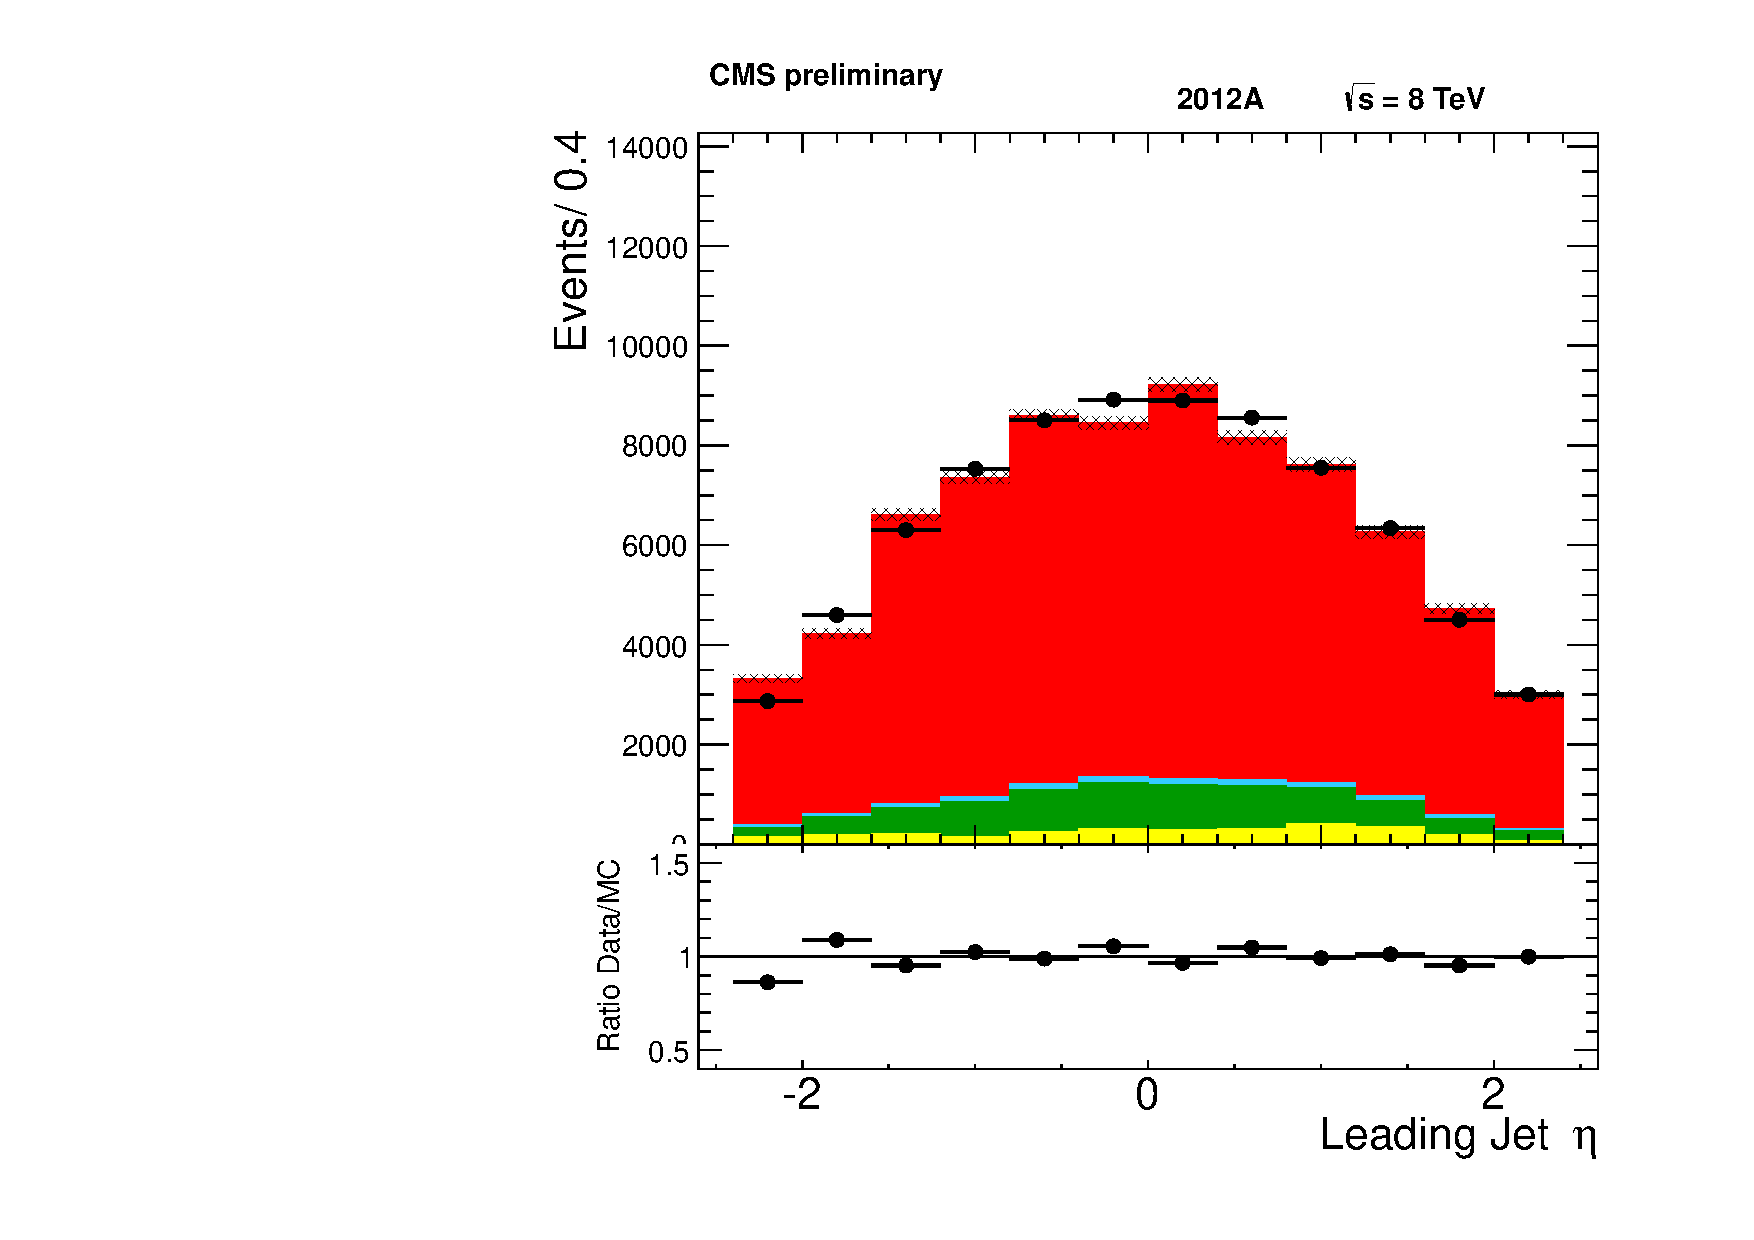
\includegraphics[width=0.3\textwidth]{plots/mu_jetld_eta_2012A.pdf}
    }
    \subfigure[2012B: leading jet $\eta$]{
      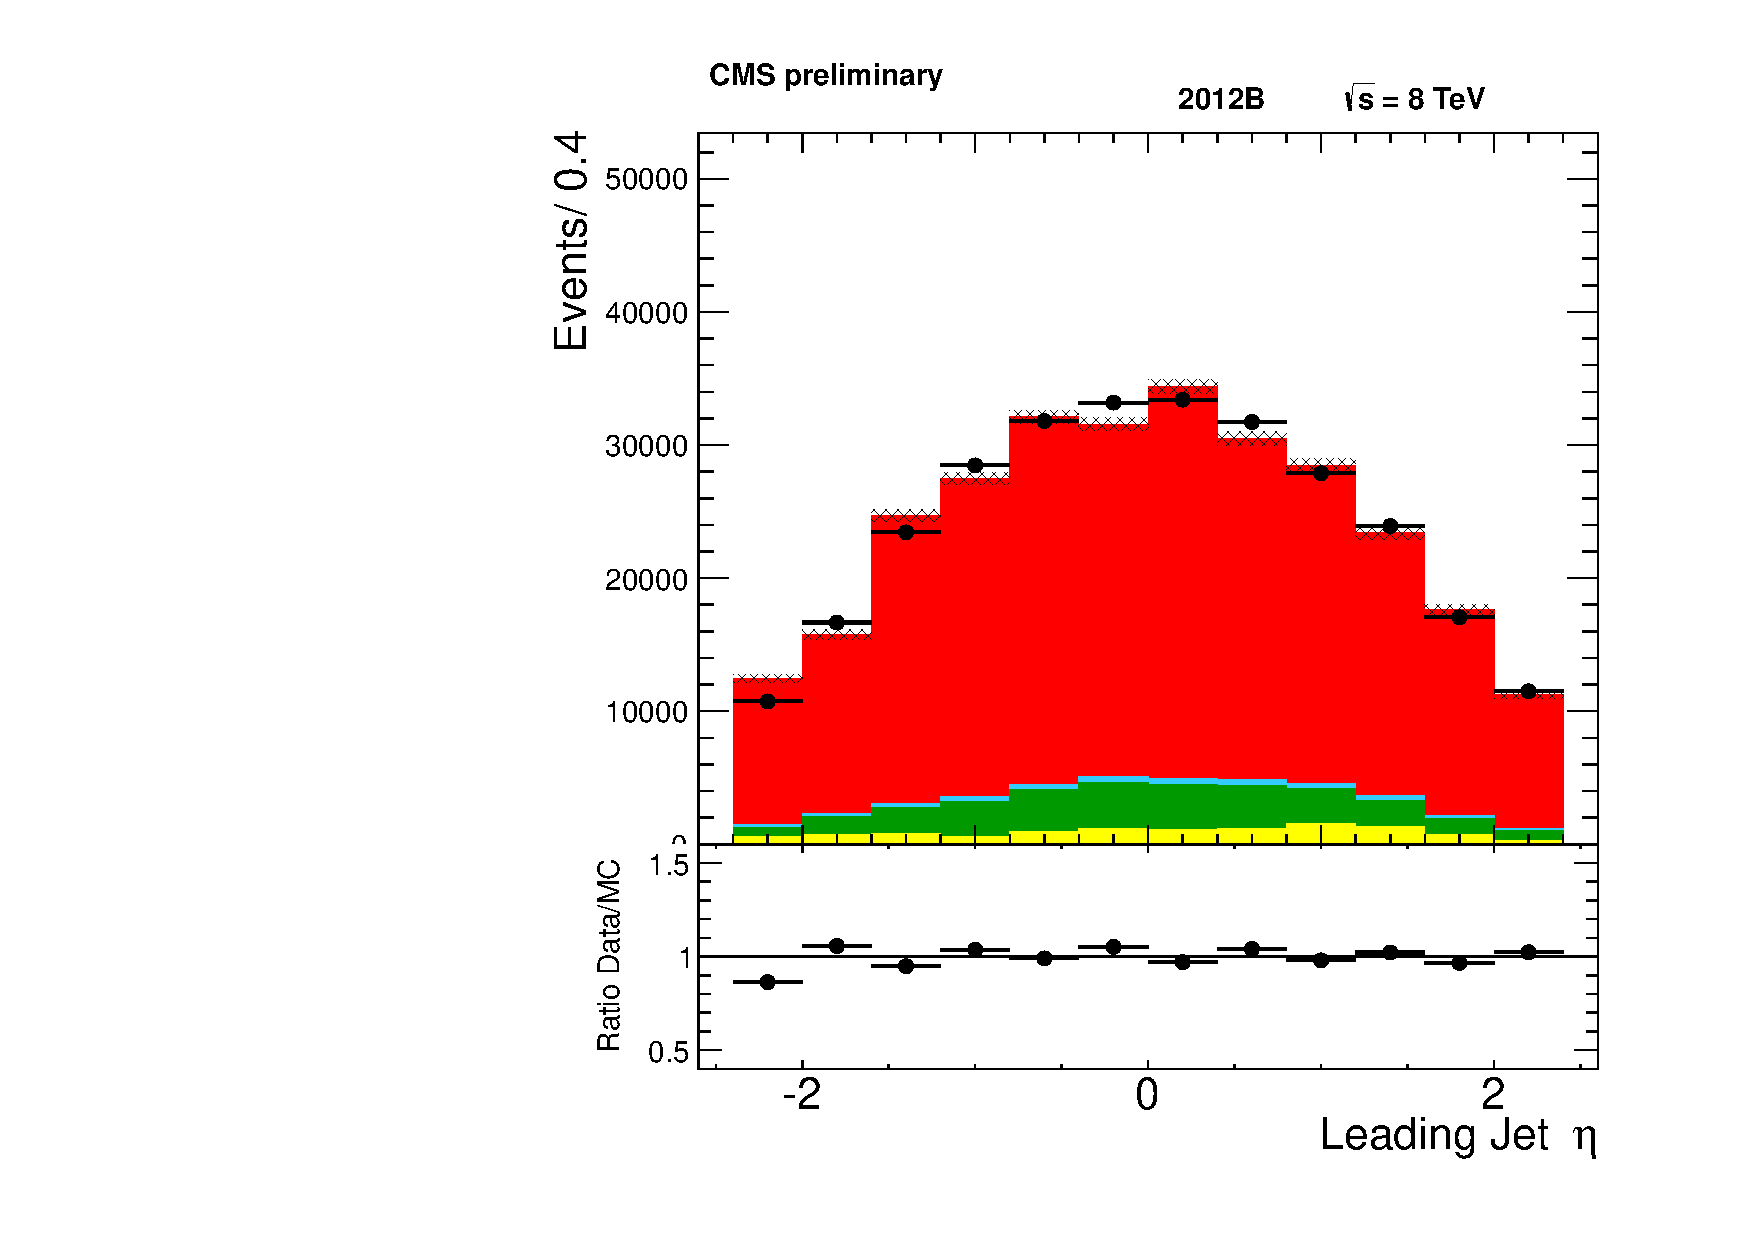
\includegraphics[width=0.3\textwidth]{plots/mu_jetld_eta_2012B.pdf}
    }
    \\
    \subfigure[2012A: second jet $\eta$ ]{
      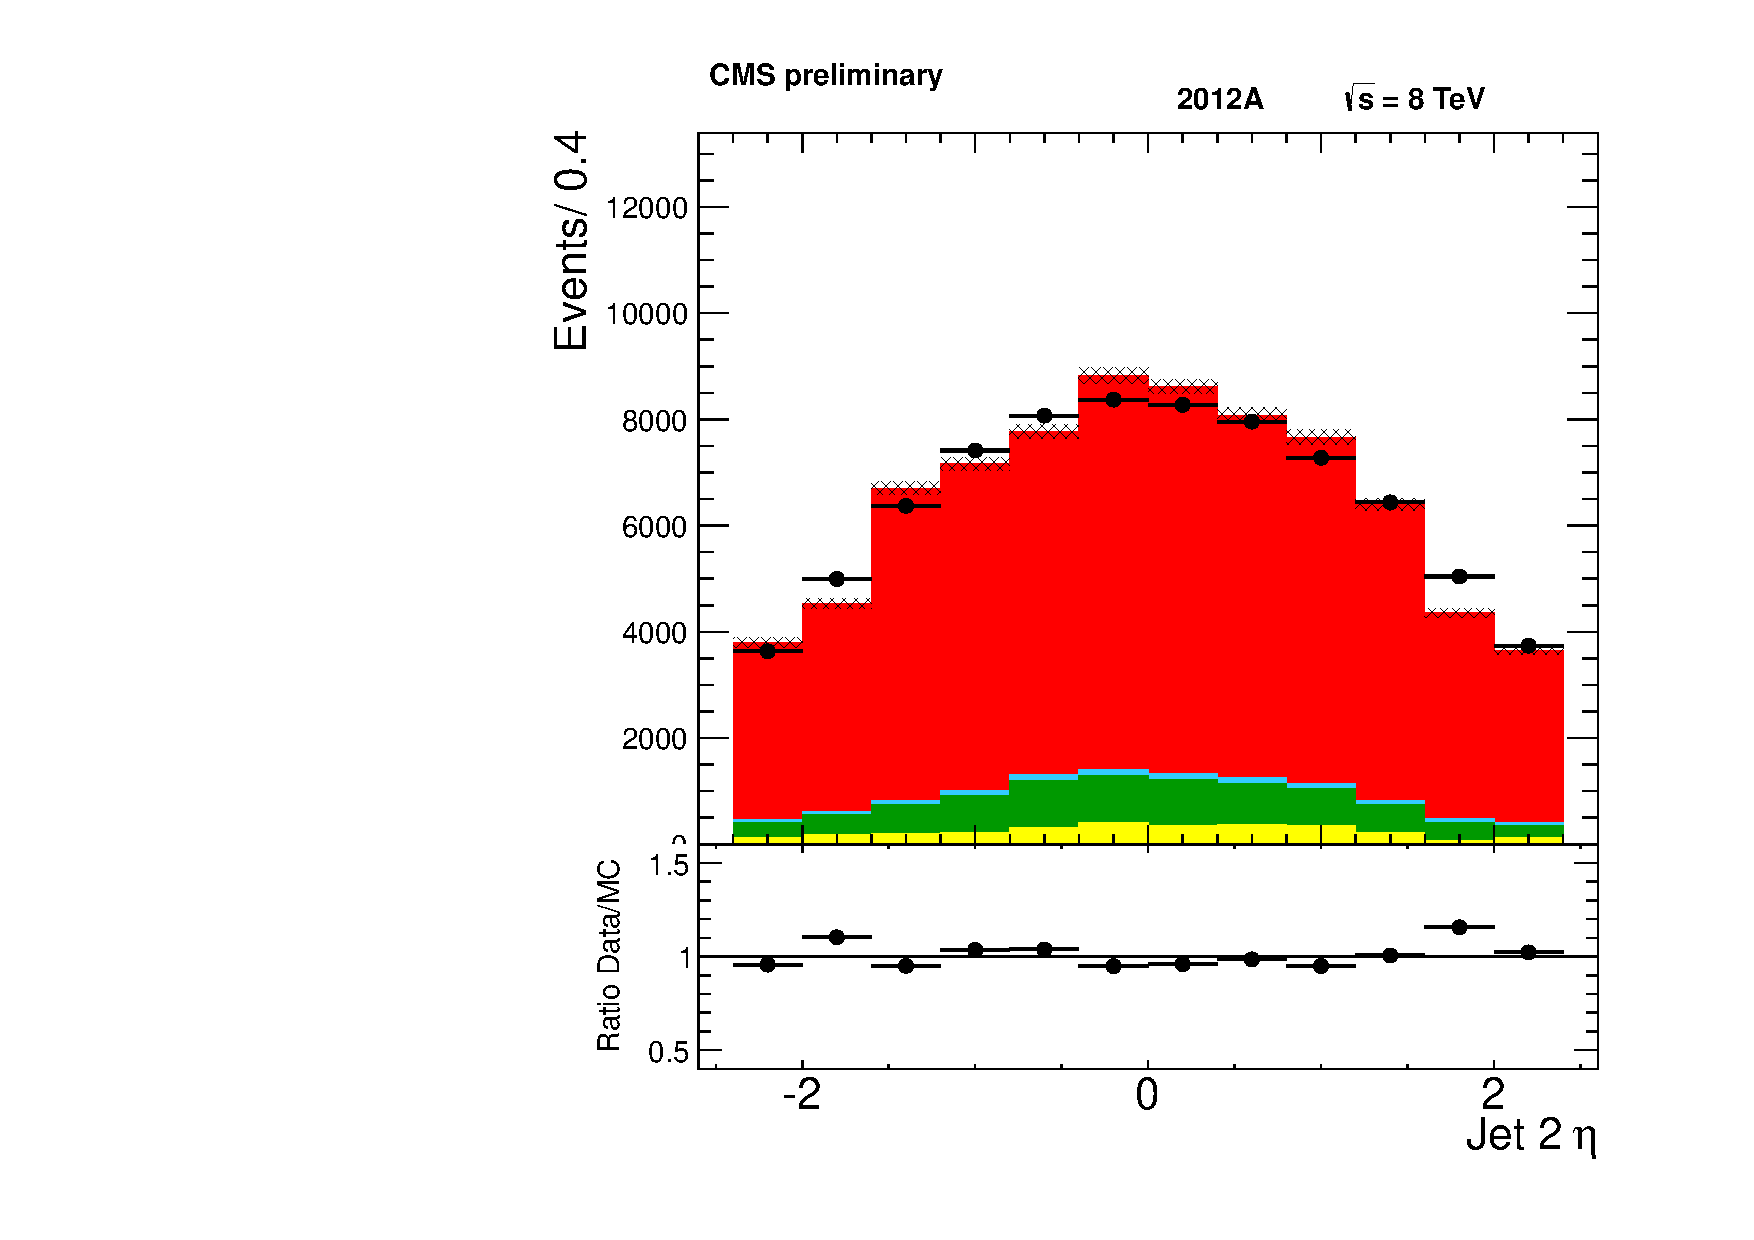
\includegraphics[width=0.3\textwidth]{plots/mu_jetnt_eta_2012A.pdf}
    }
    \subfigure[2012B: second jet $\eta$]{
      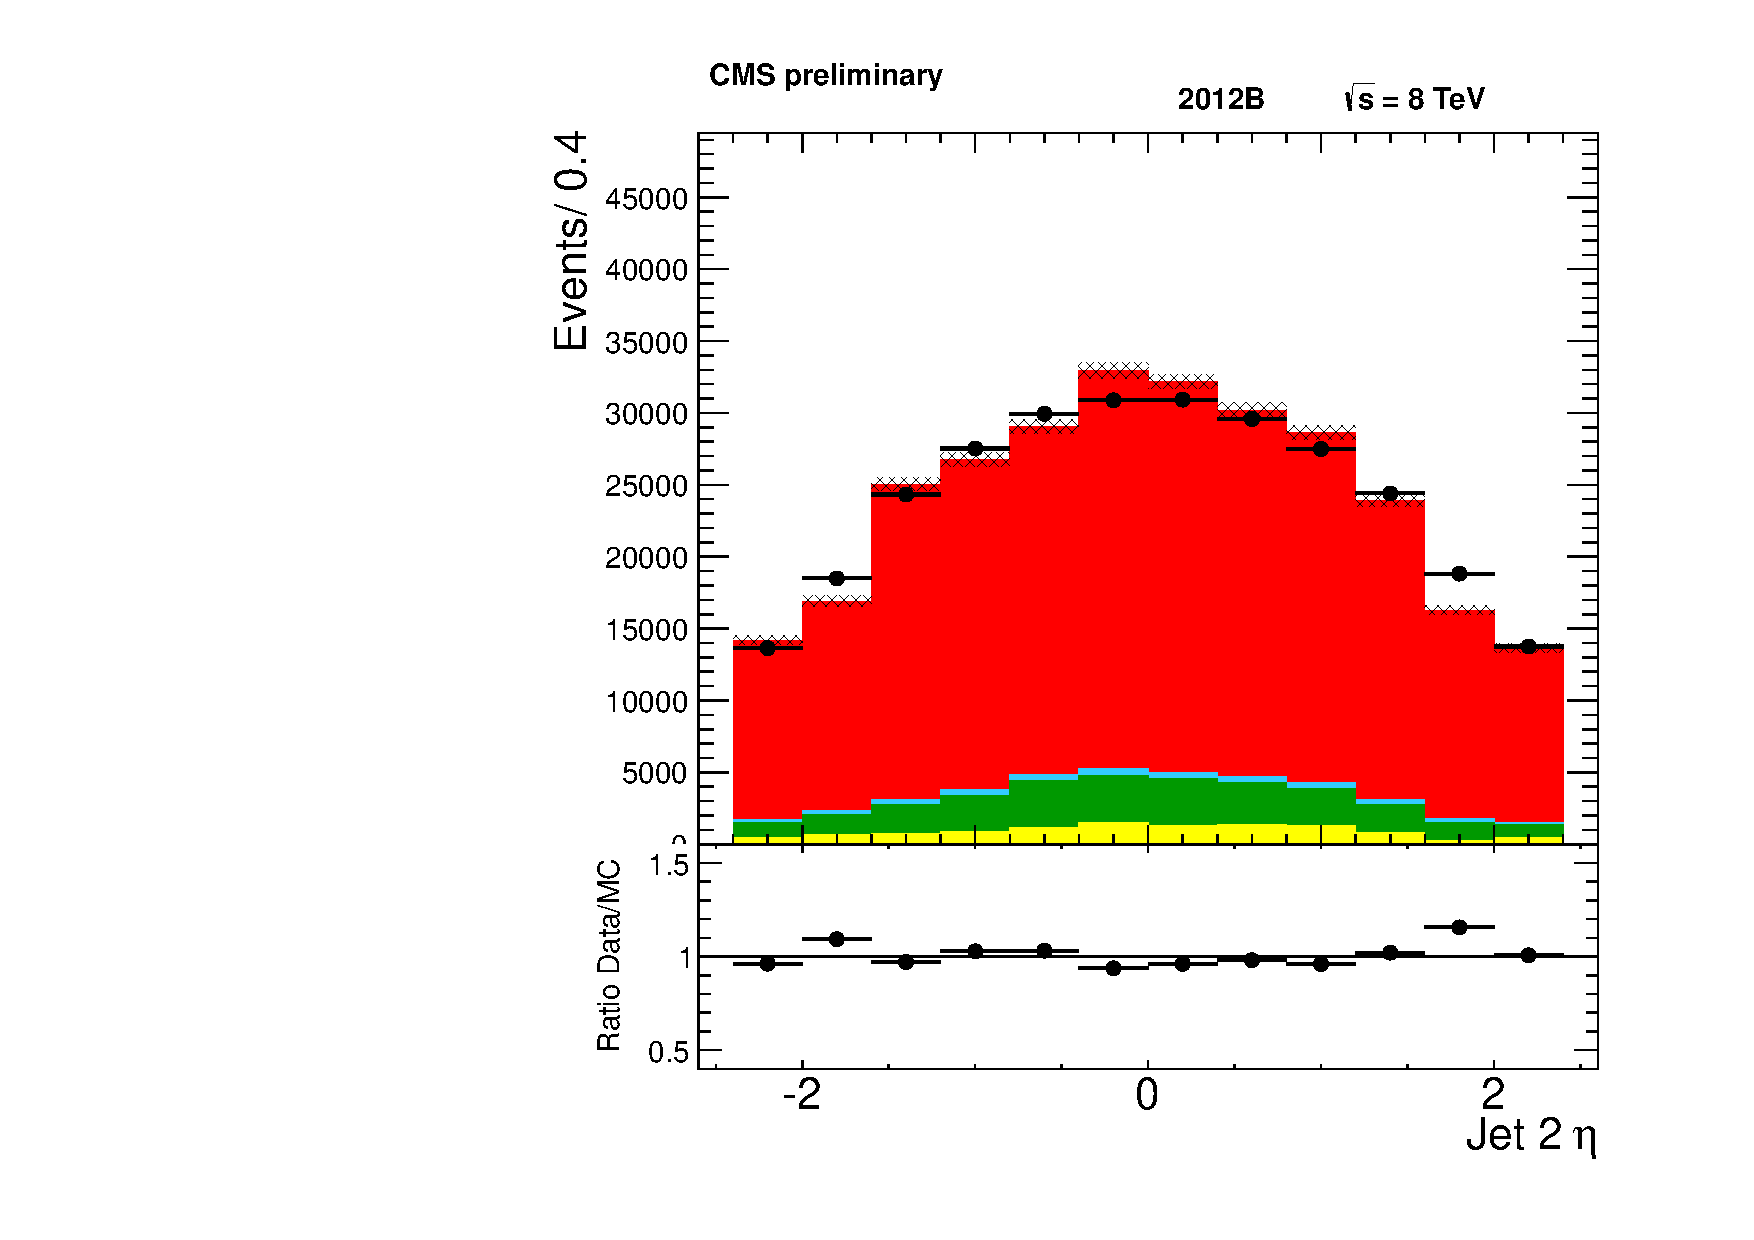
\includegraphics[width=0.3\textwidth]{plots/mu_jetnt_eta_2012B.pdf}
    }
    \caption{
             Comparison of the leading jet and second jet $p_{T}$ and $\eta$ distributions from data and MC for the muon+jets
      selection.
            }
    \label{fig:CP2012AB1}
\end{figure}


\begin{figure}[htb]
  \centering
    \subfigure[2012A: muon $p_{T}$]{
      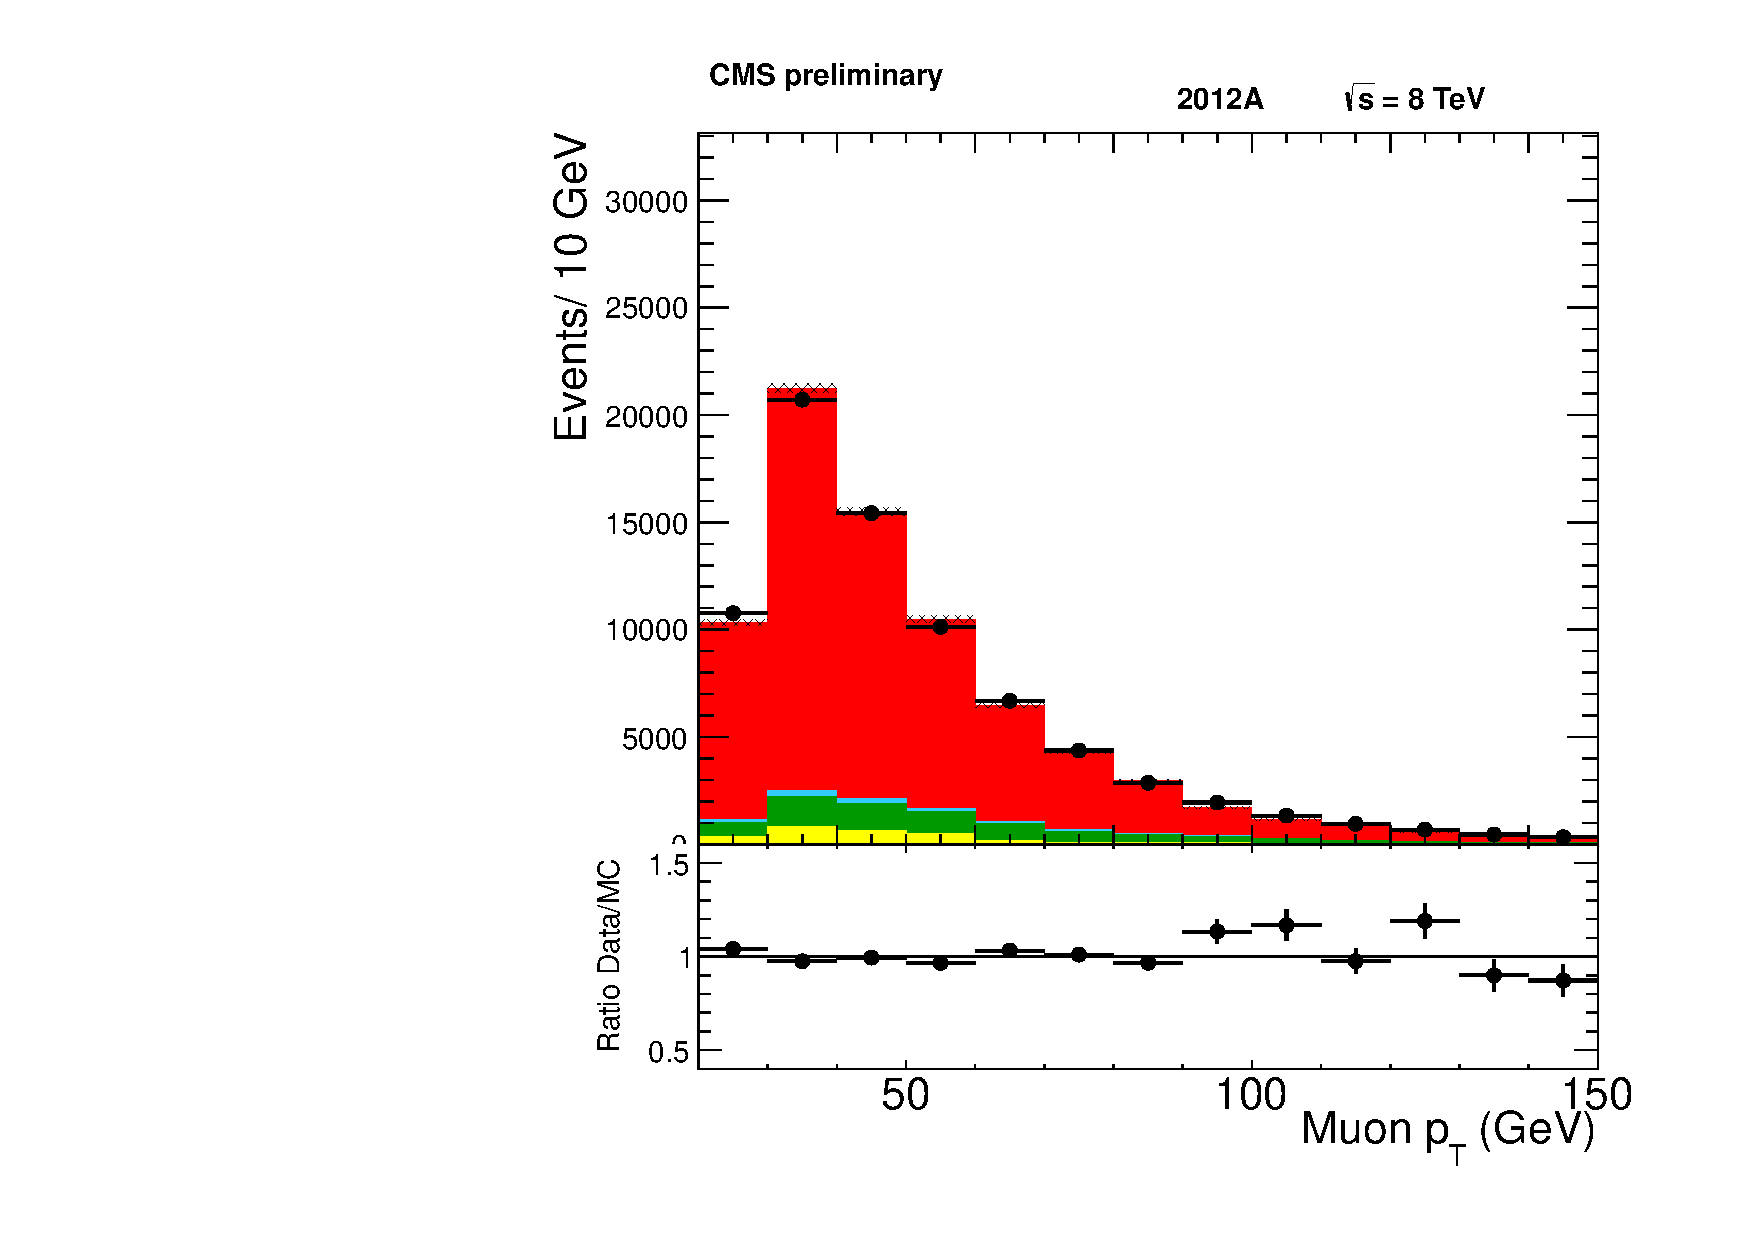
\includegraphics[width=0.4\textwidth]{plots/mu_W_muon_pt_2012A.pdf}
    }
    \subfigure[2012B: muon $p_{T}$]{
      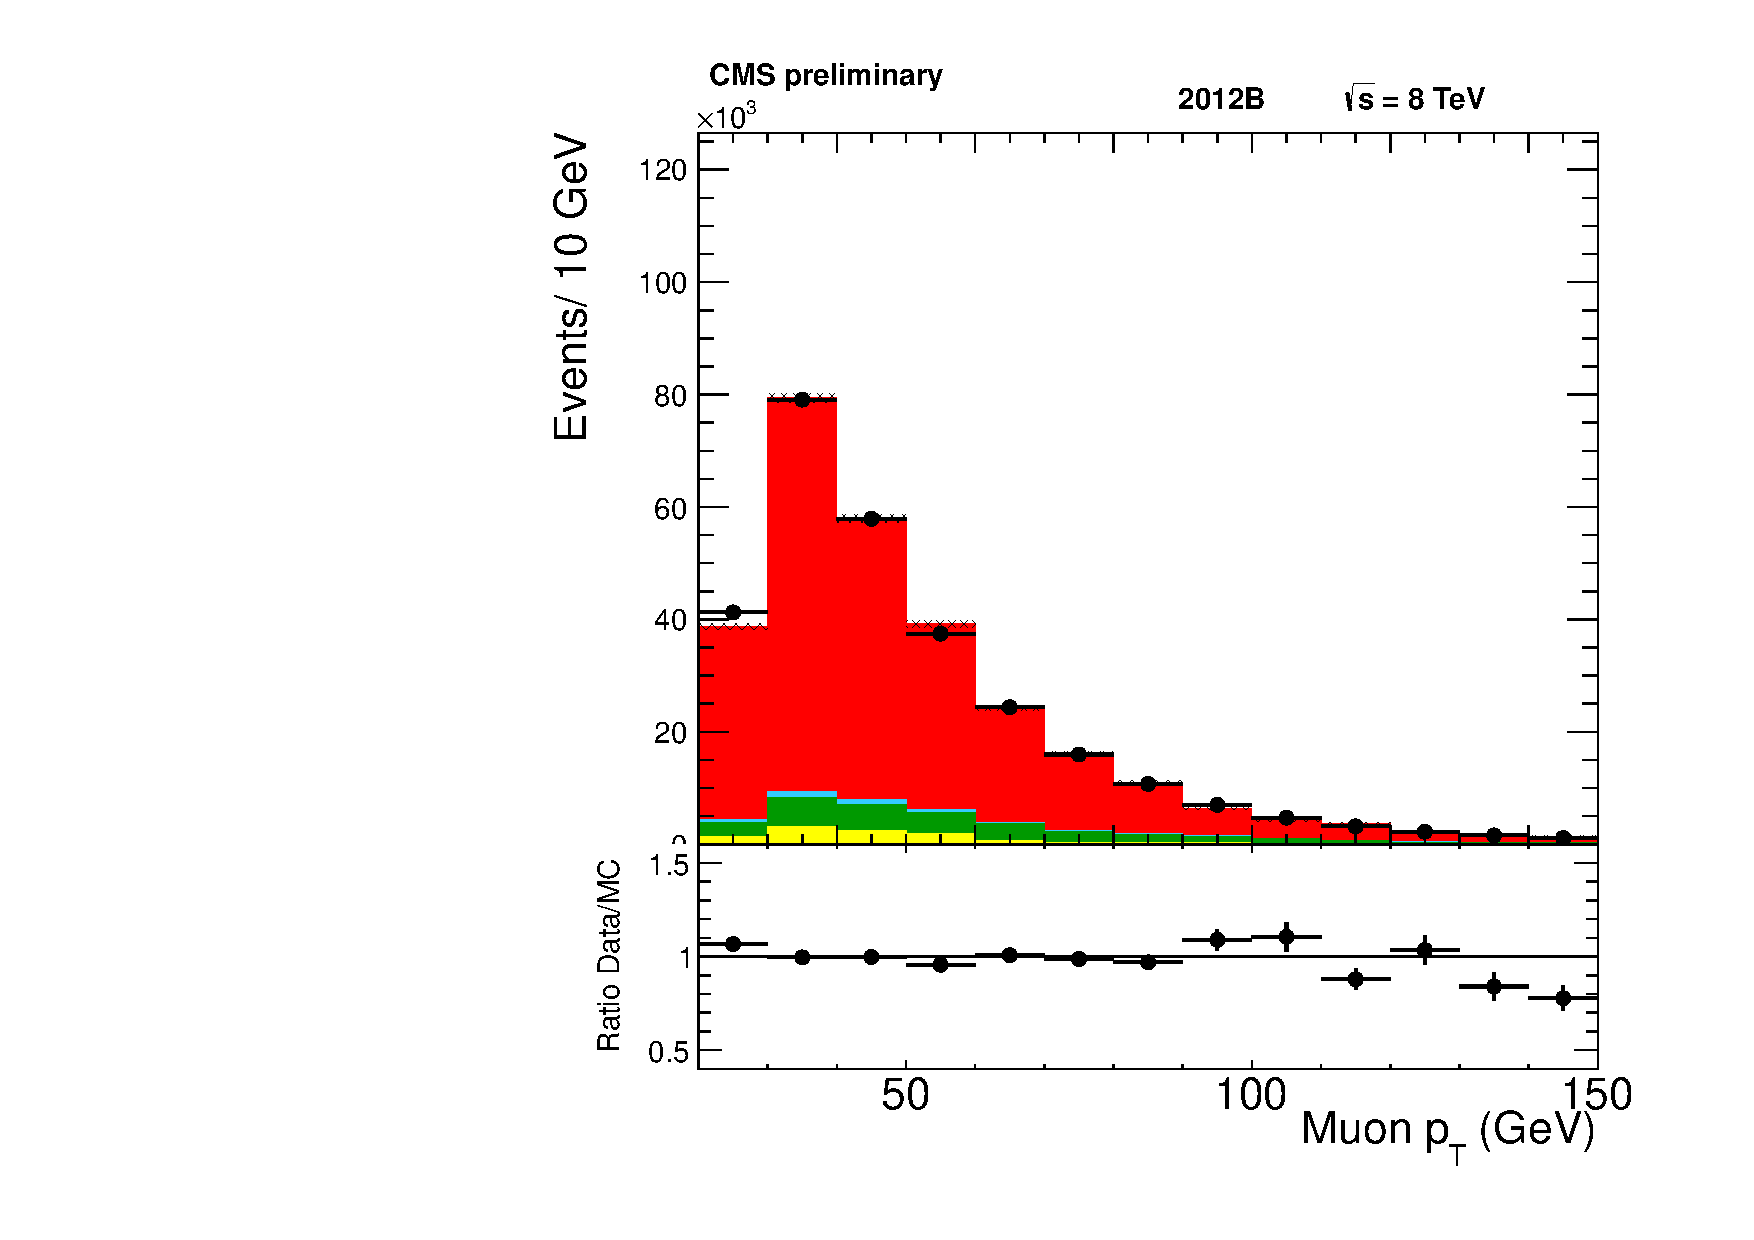
\includegraphics[width=0.4\textwidth]{plots/mu_W_muon_pt_2012B.pdf}
    }
    \\
    \subfigure[2012A: muon $\eta$]{
      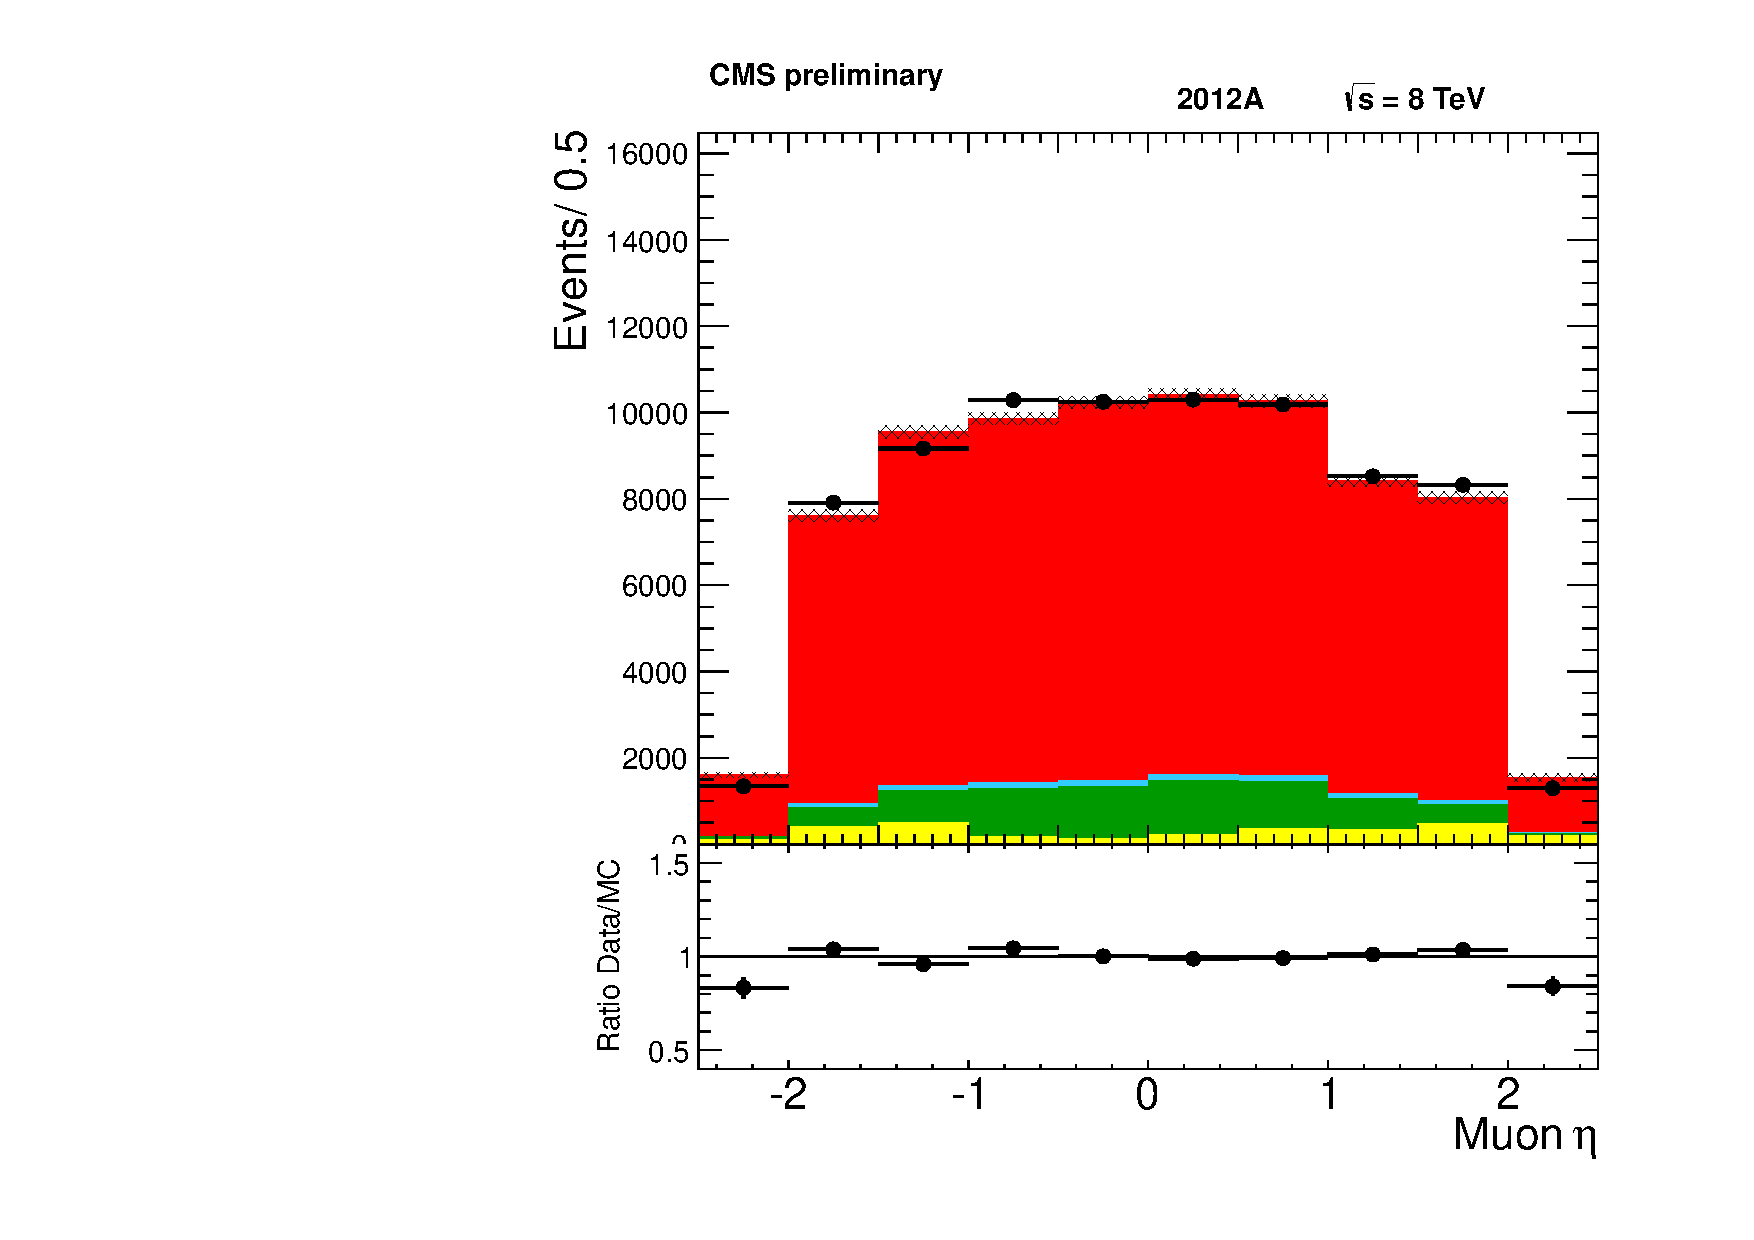
\includegraphics[width=0.4\textwidth]{plots/mu_W_muon_eta_2012A.pdf}
    }
    \subfigure[2012B: muon $\eta$]{
      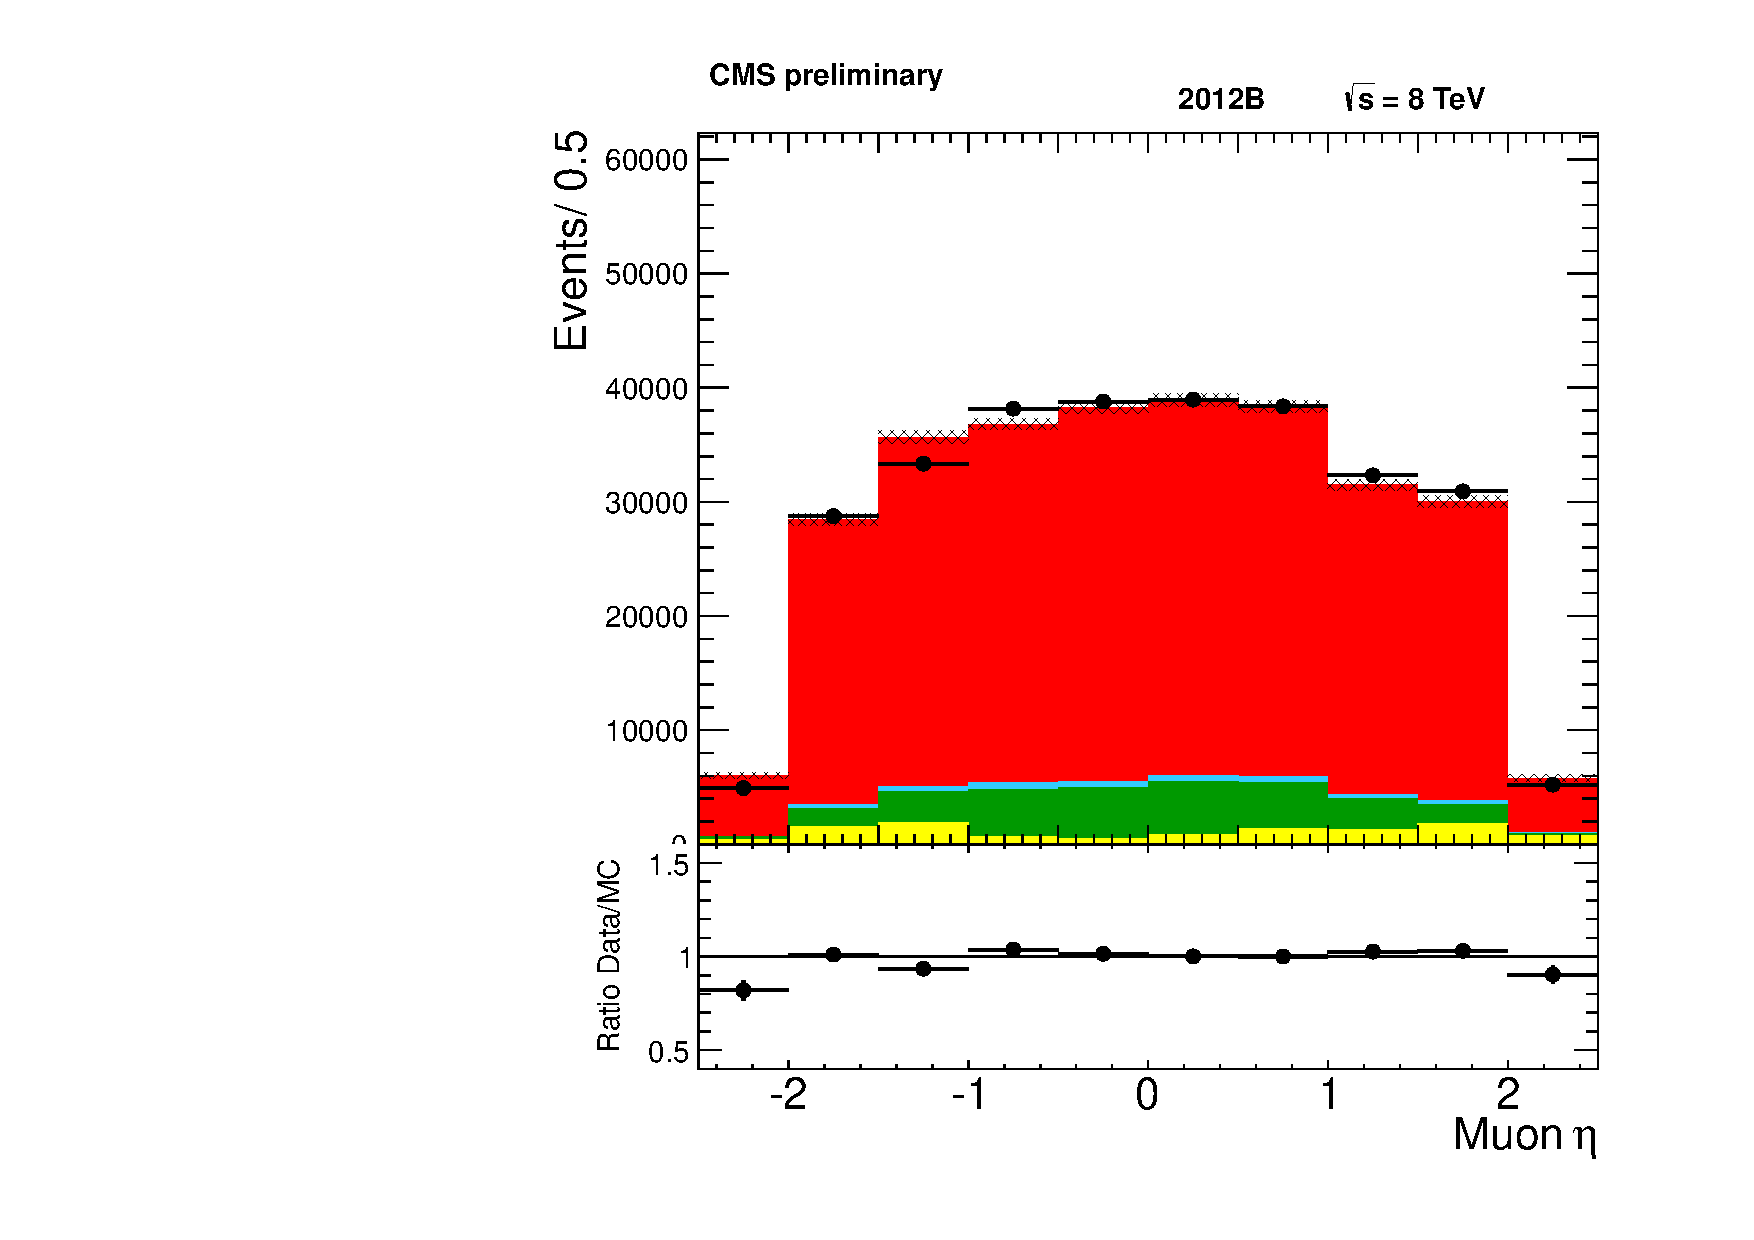
\includegraphics[width=0.4\textwidth]{plots/mu_W_muon_eta_2012B.pdf}
    }
    \\
    \subfigure[2012A: $M_{T}$]{
      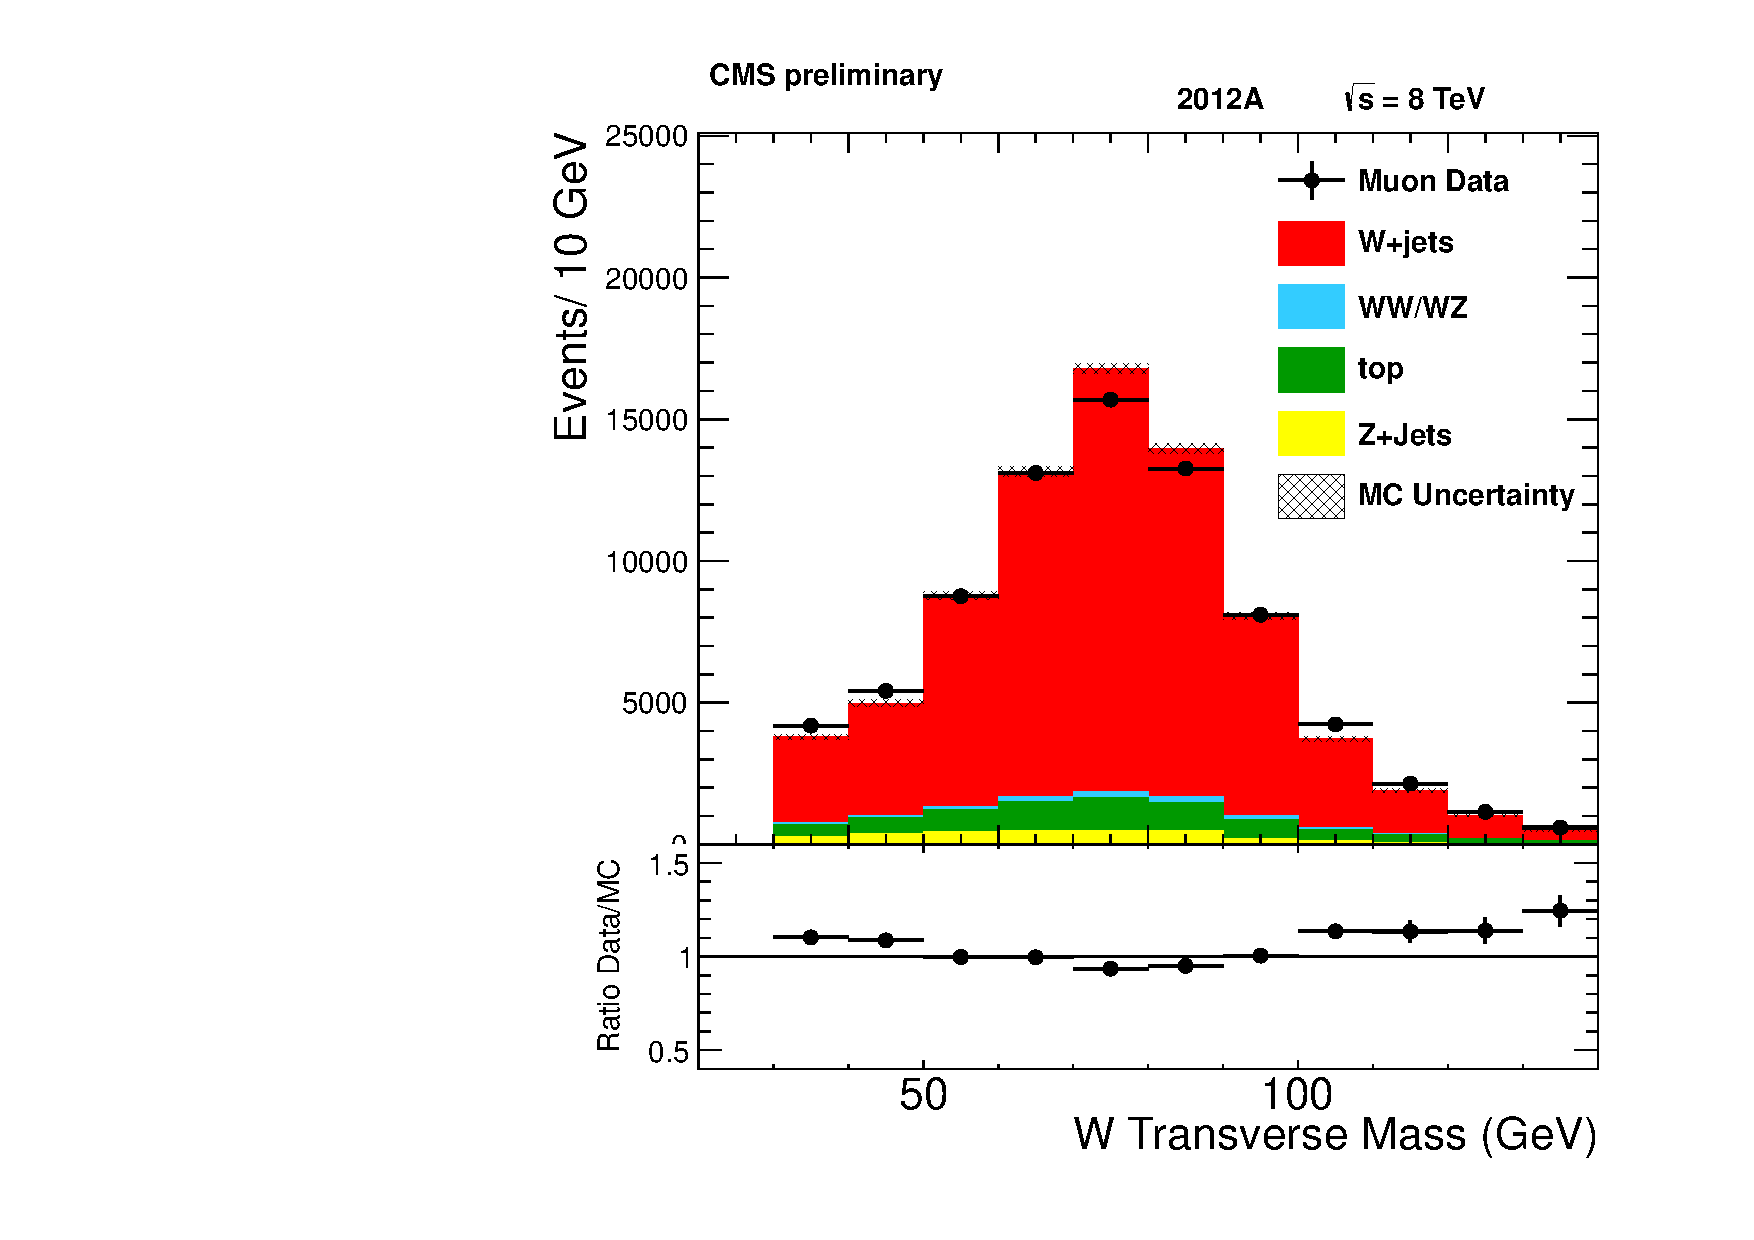
\includegraphics[width=0.4\textwidth]{plots/mu_W_mt_2012A.pdf}
    }
    \subfigure[2012B: $M_{T}$]{
      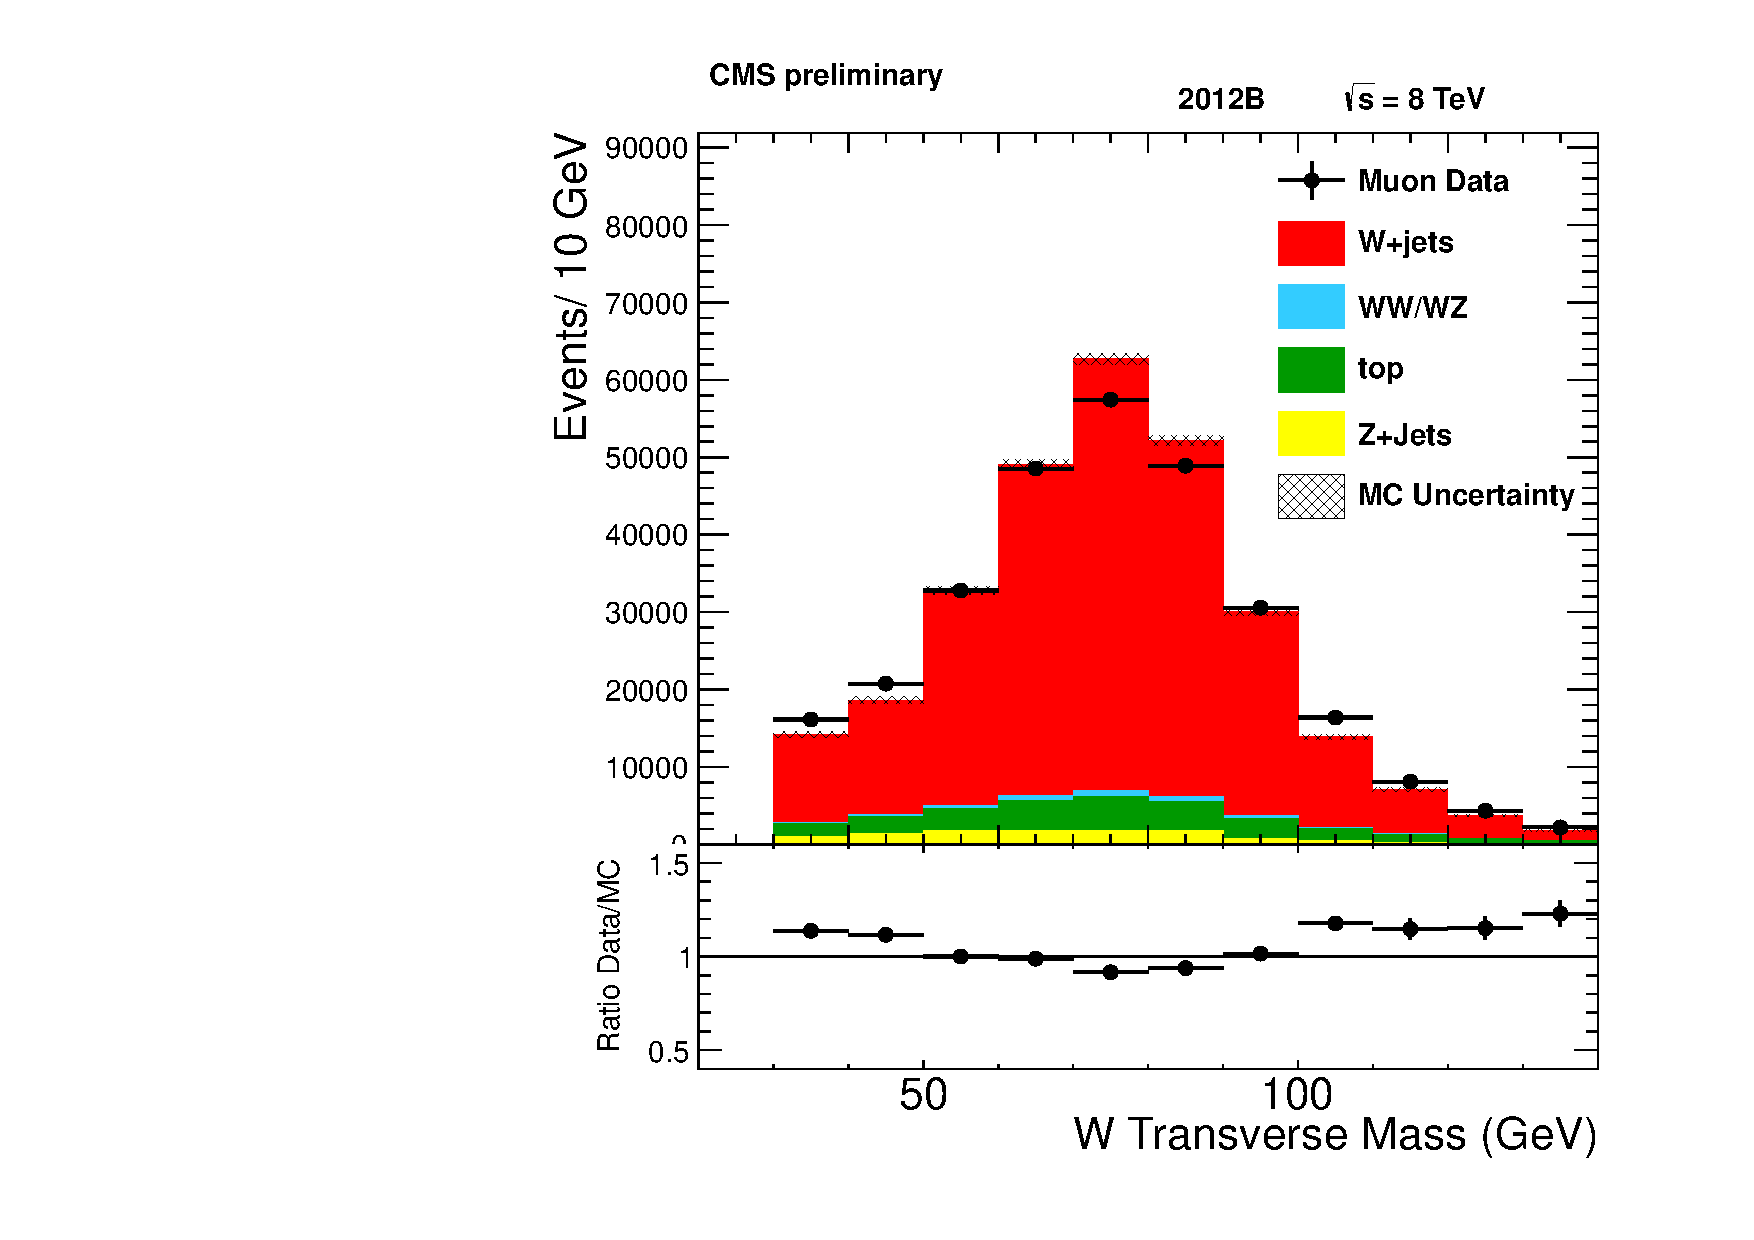
\includegraphics[width=0.4\textwidth]{plots/mu_W_mt_2012B.pdf}
    }
    \\
    \caption{
             Comparison of the muon $p_{T}$, $\eta$ and the transverse mass of the muon / MET system distributions from data and MC for the 
muon+jets selection.
            }
    \label{fig:CP2012AB2}
\end{figure}

\begin{figure}[htb]
  \centering
    \subfigure[2012A: MET]{
      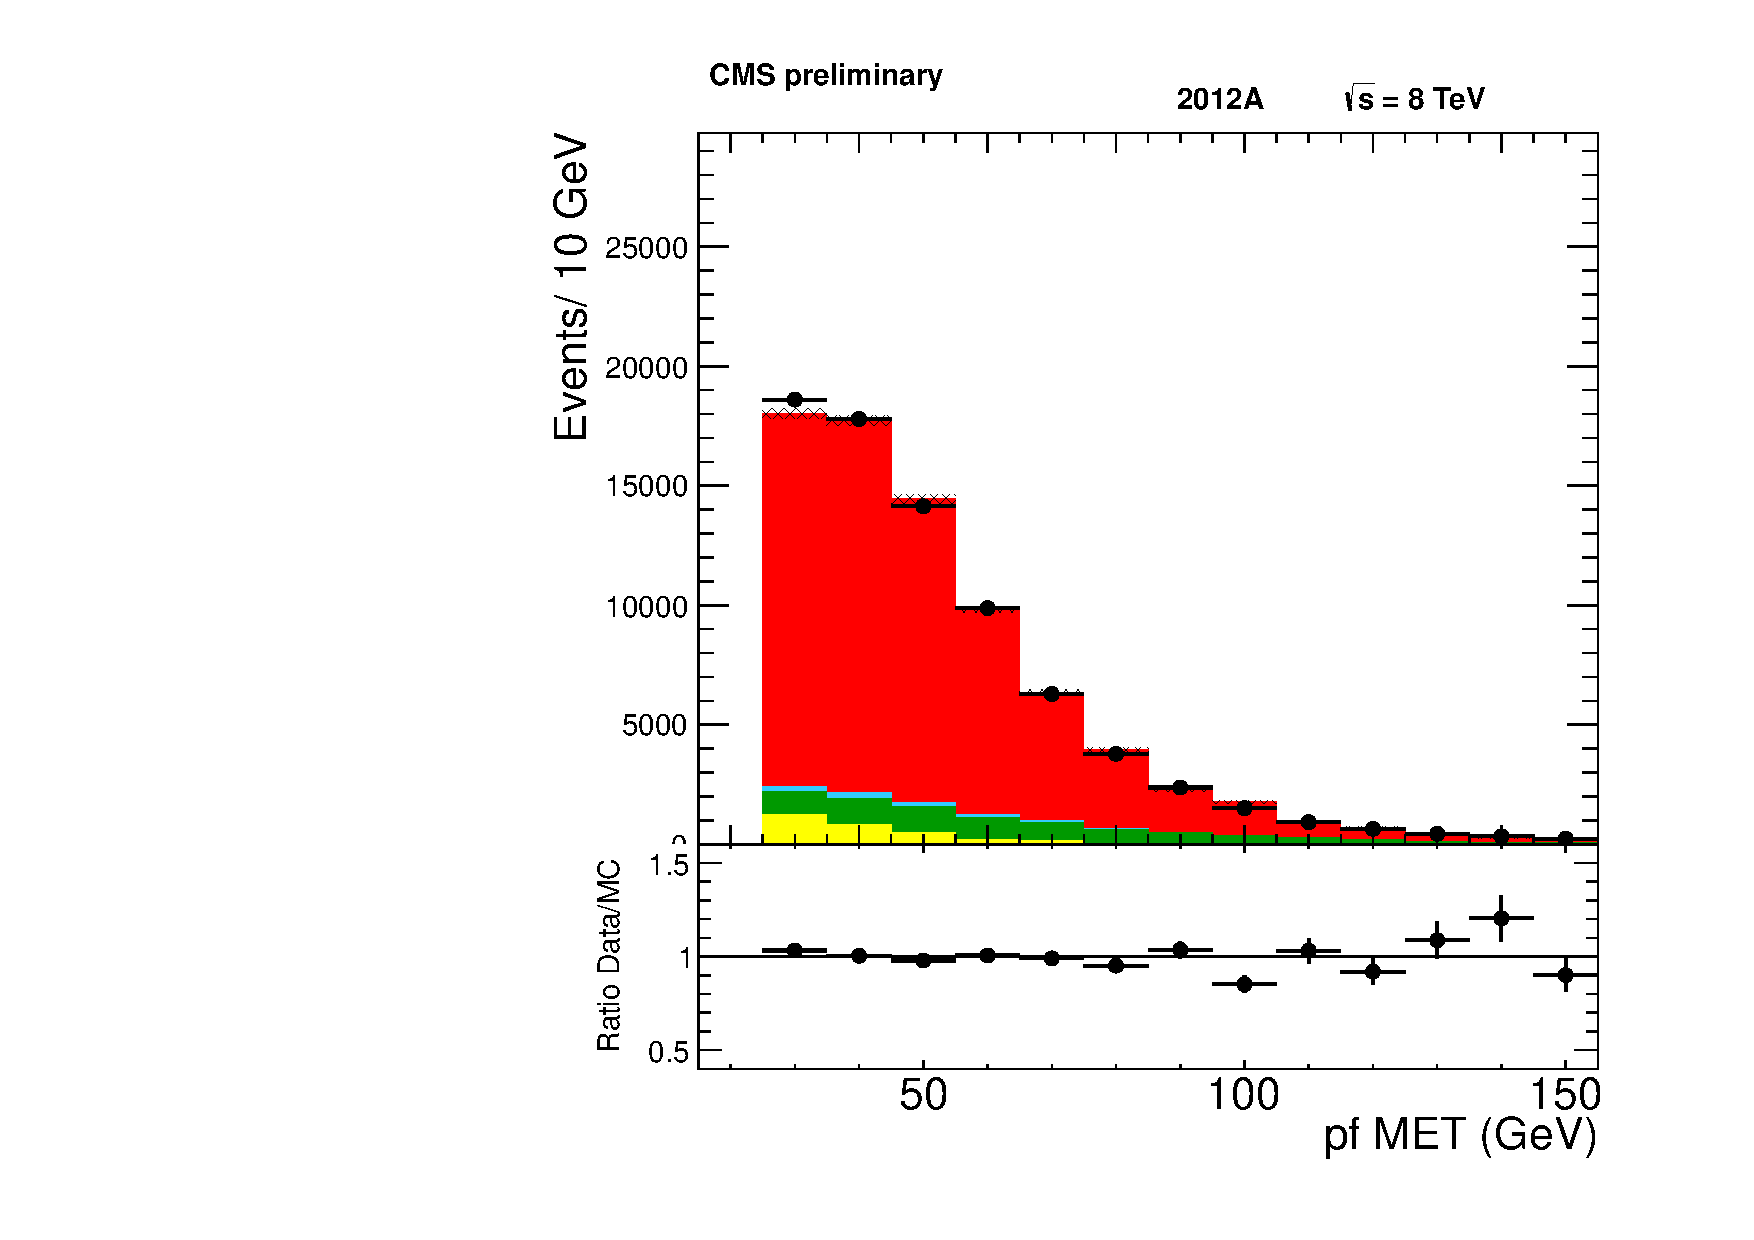
\includegraphics[width=0.4\textwidth]{plots/mu_event_met_pfmet_2012A.pdf}
    }
    \subfigure[2012B: MET]{
      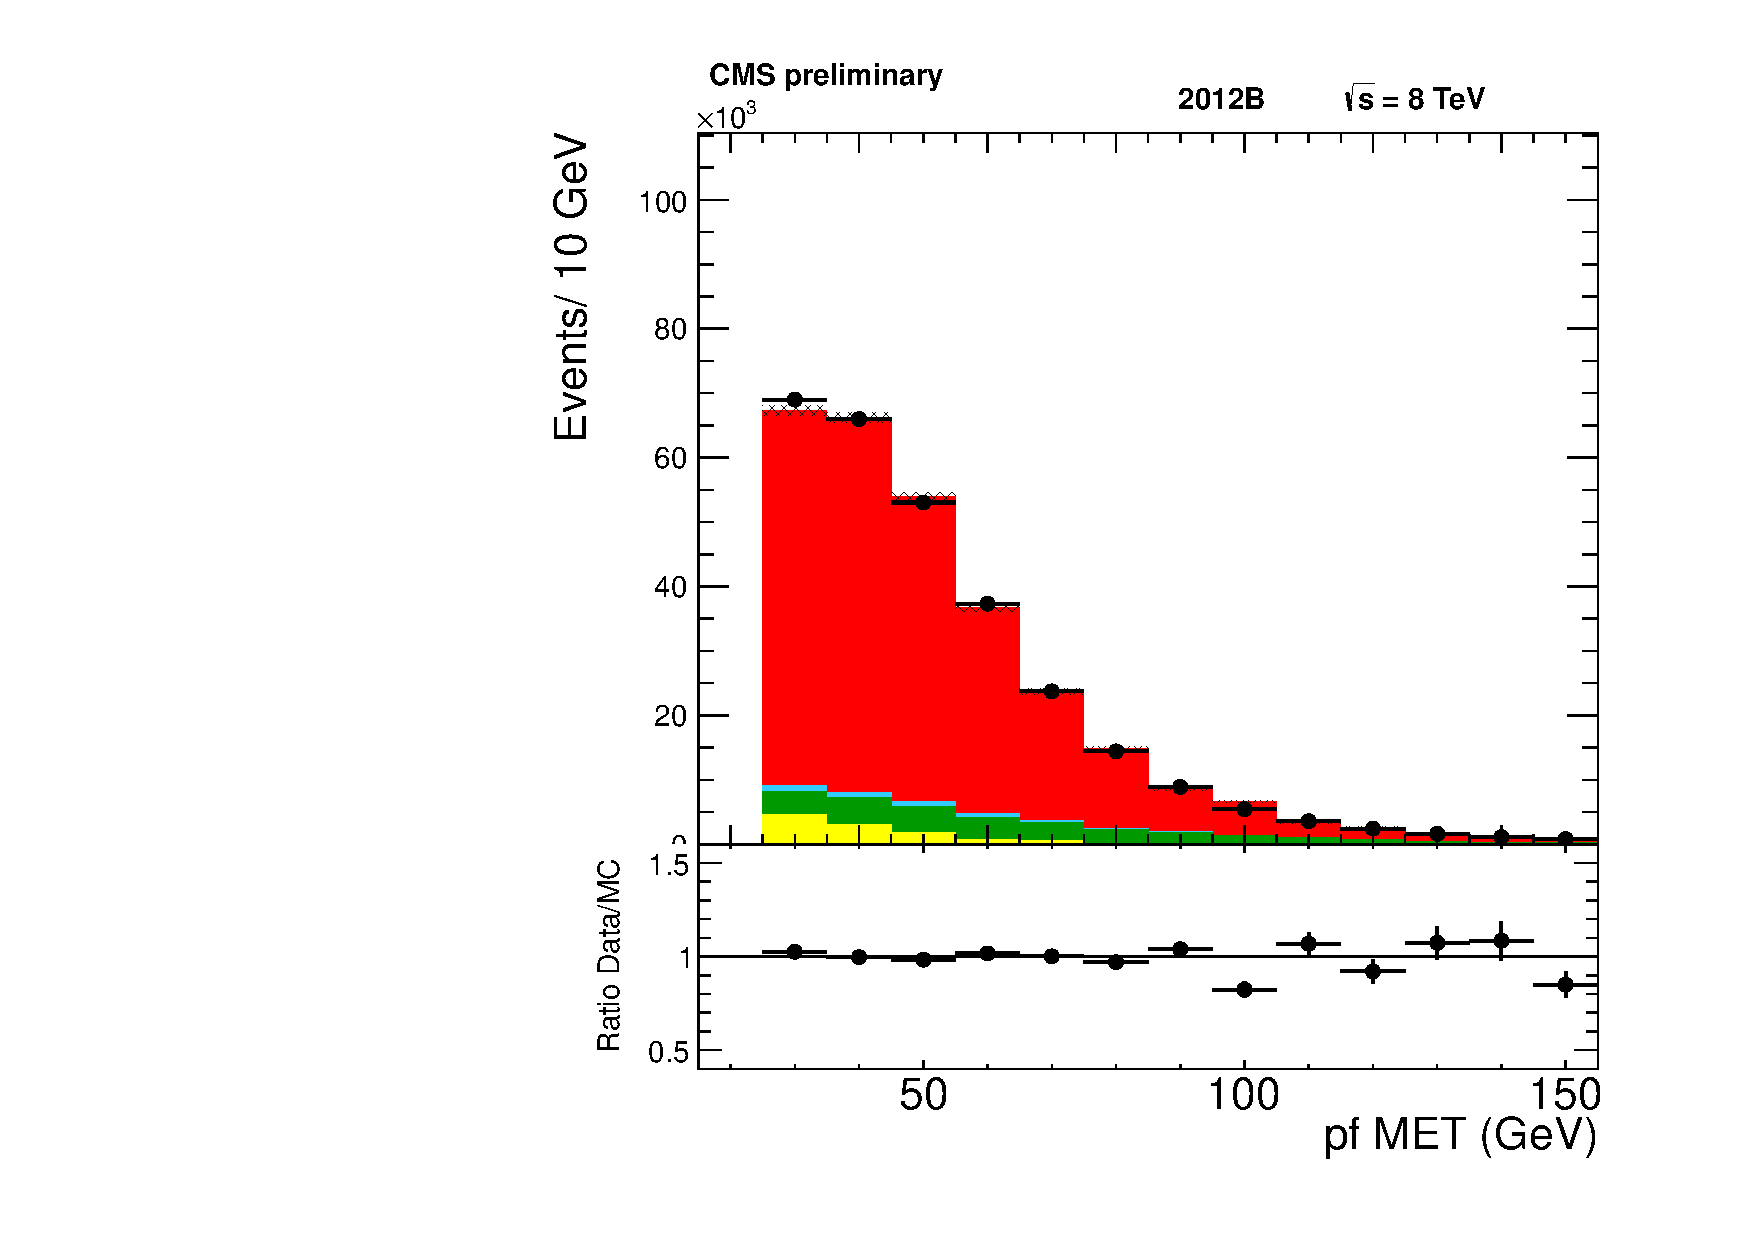
\includegraphics[width=0.4\textwidth]{plots/mu_event_met_pfmet_2012B.pdf}
    }
    \\
    \subfigure[2012A: dijet mass($m_{jj}$)]{
      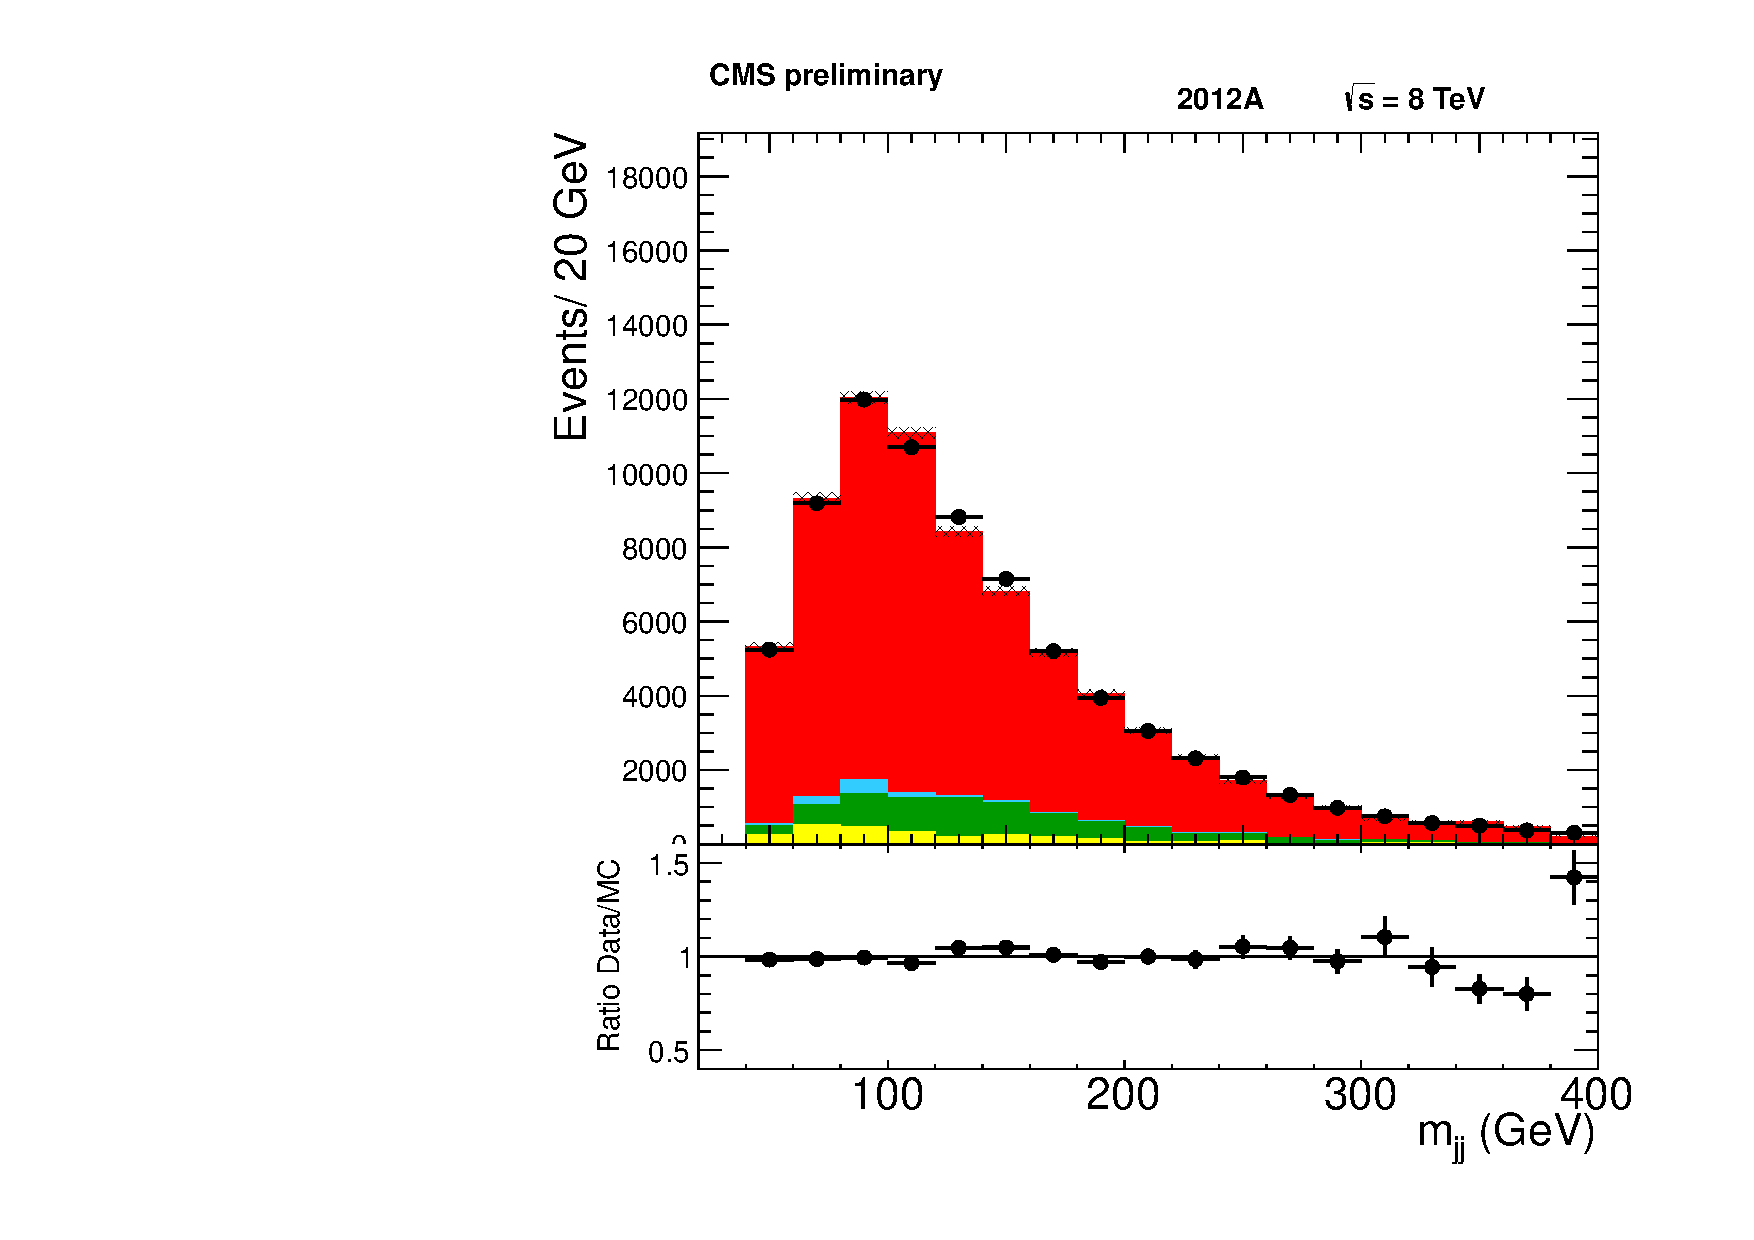
\includegraphics[width=0.4\textwidth]{plots/mu_mjj_2012A.pdf}
    }
    \subfigure[2012B: dijet mass($m_{jj}$)]{
      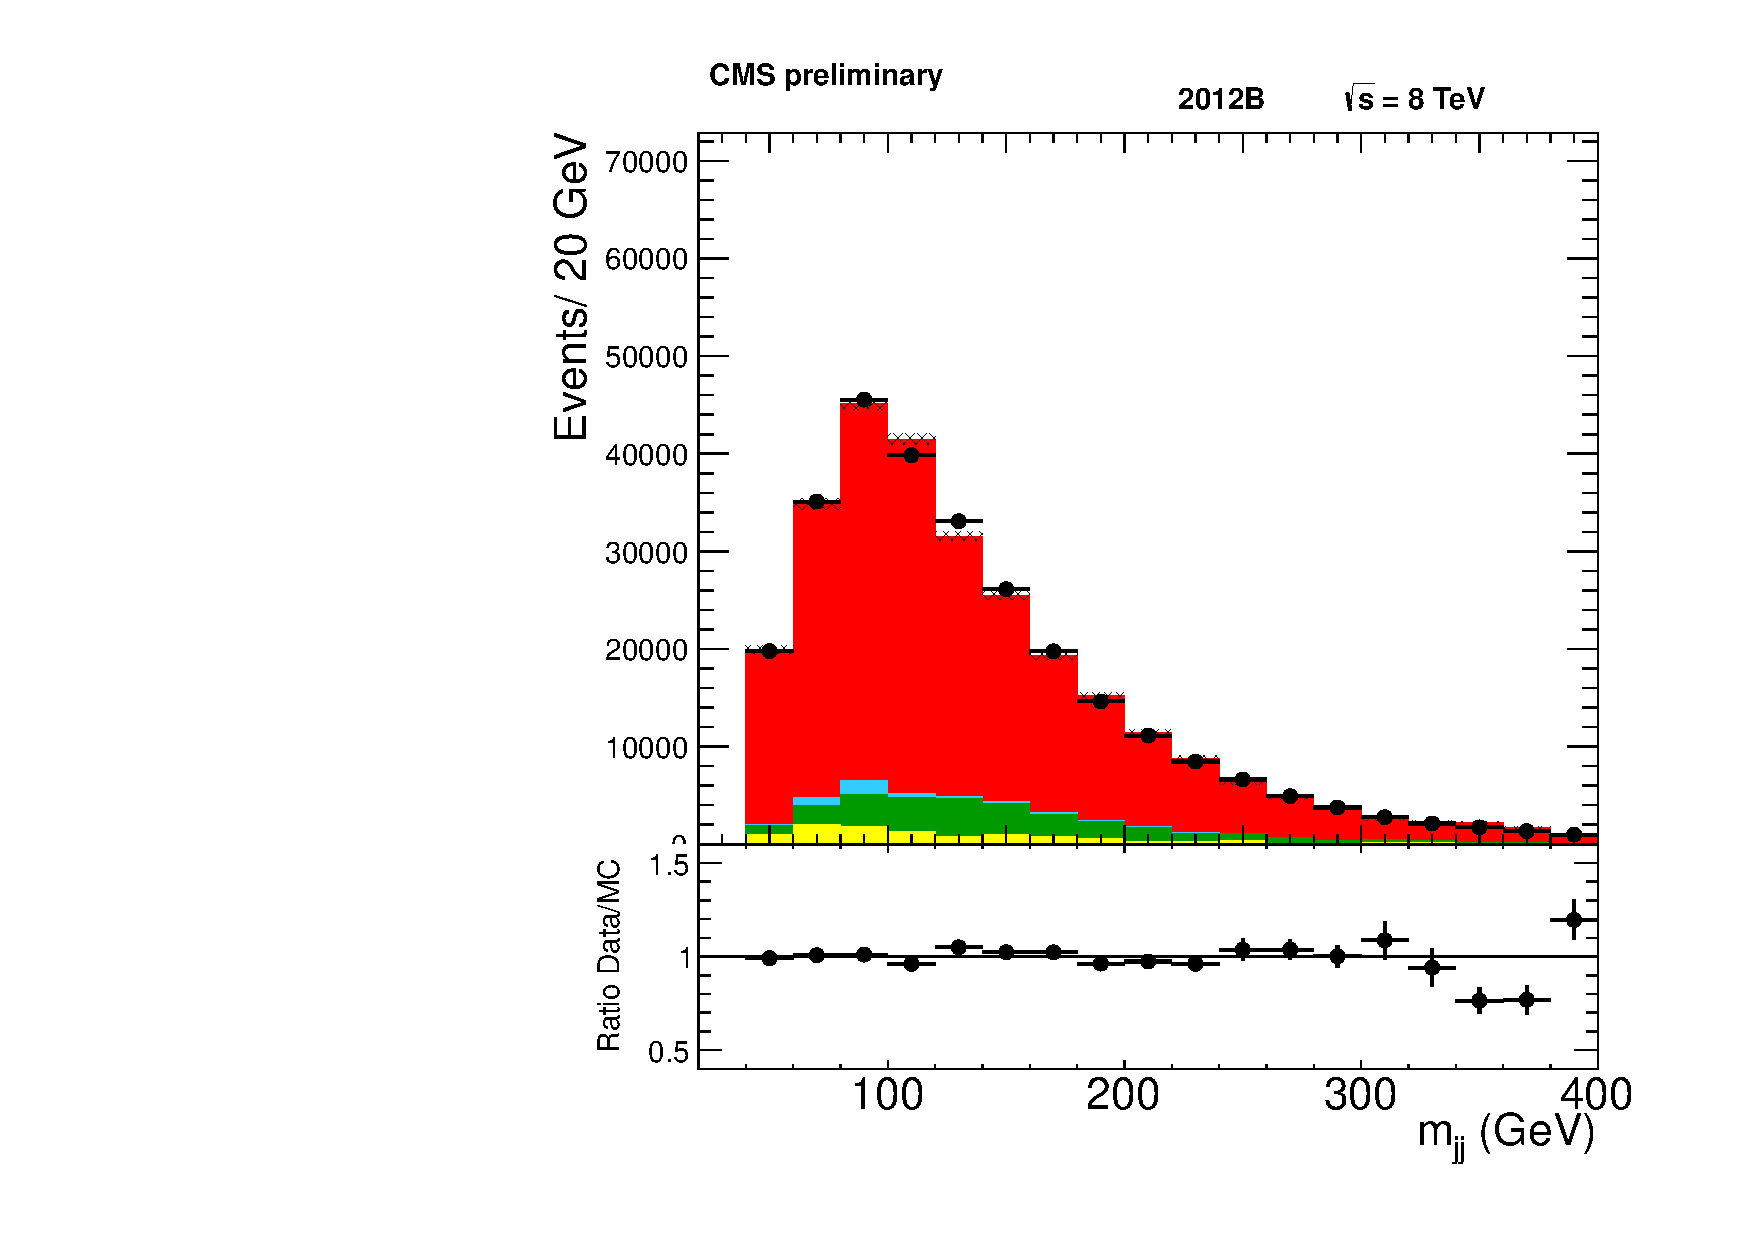
\includegraphics[width=0.4\textwidth]{plots/mu_mjj_2012B.pdf}
    }
    \\
    \caption{
             Comparison of the MET and the dijet mass($m_{jj}$) distributions from data and MC for the 
muon+jets selection.
            }
    \label{fig:CP2012AB3}
\end{figure}



\begin{figure}[htb]
  \centering
    \subfigure[2012A: leading jet $p_{T}$]{
      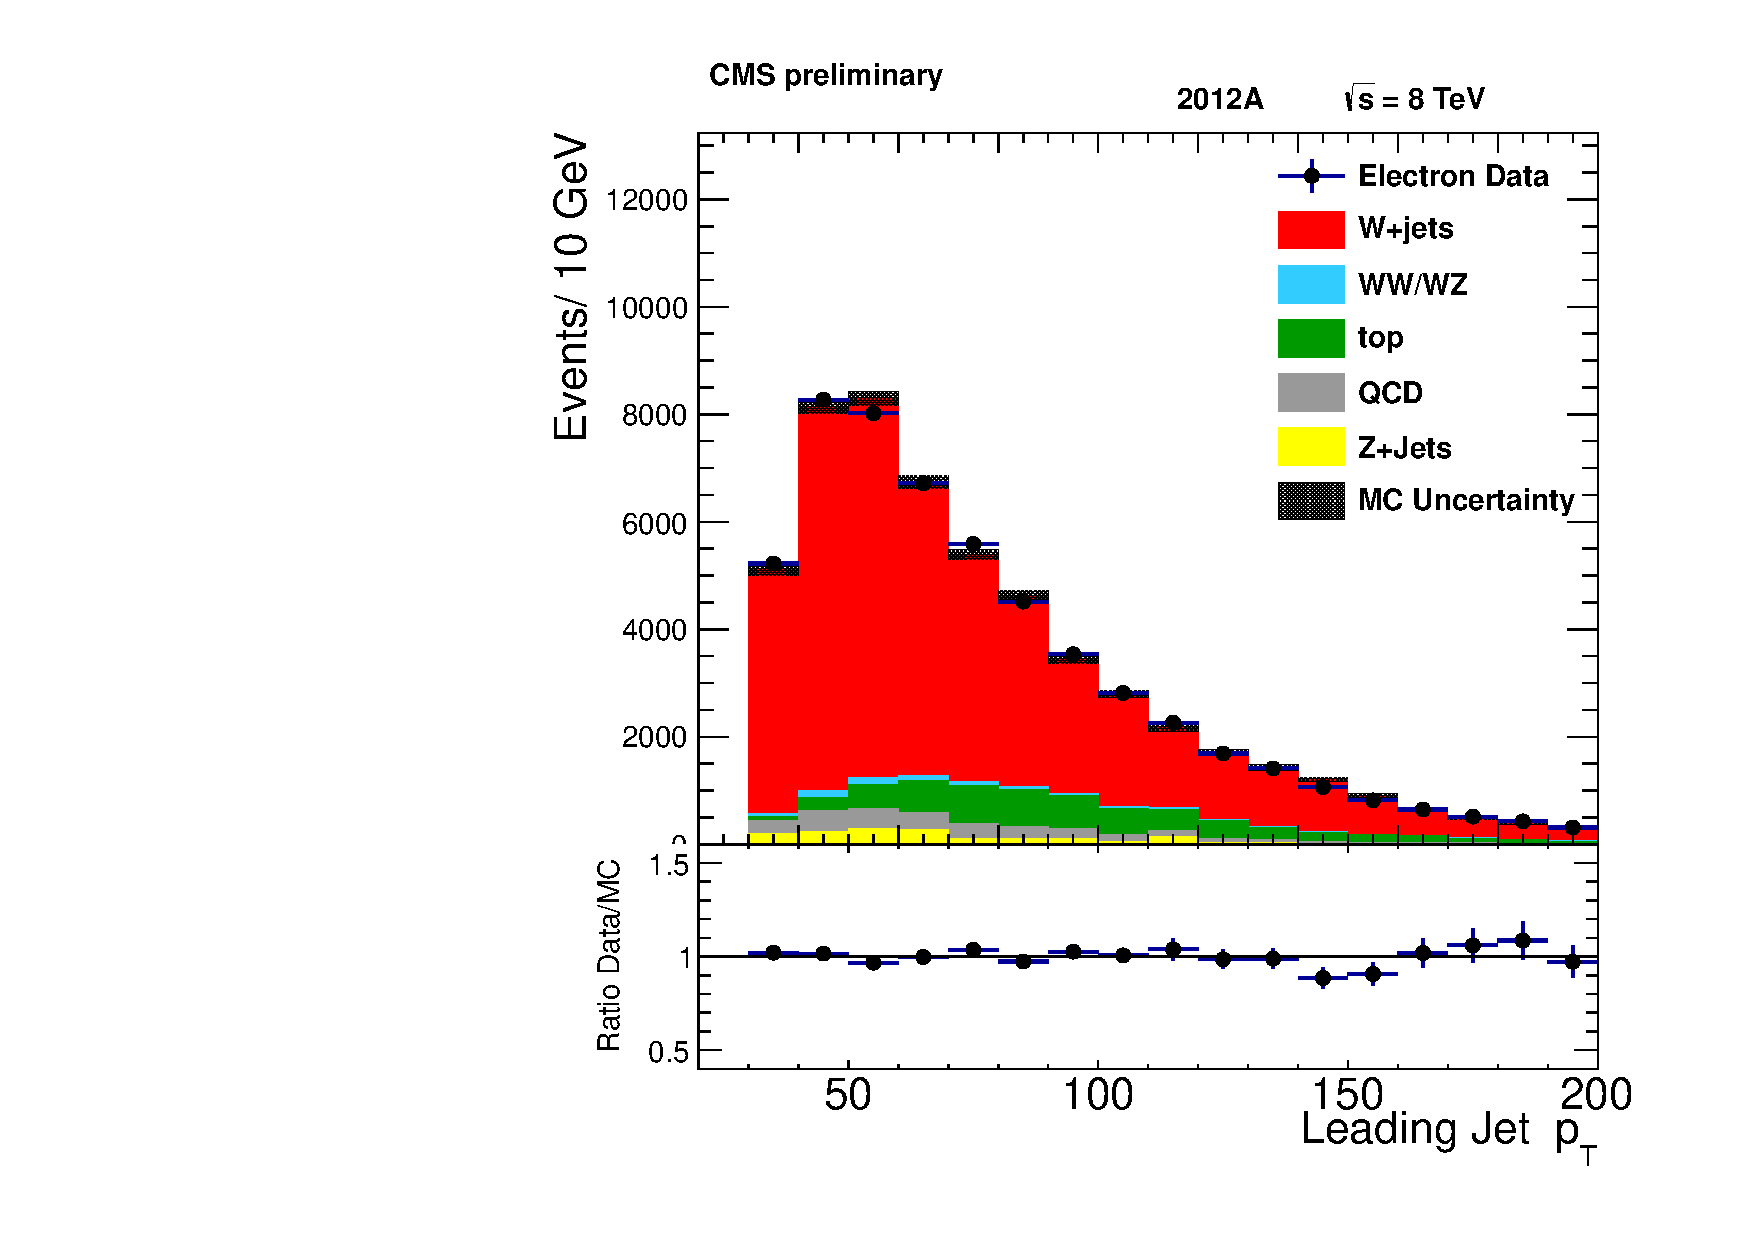
\includegraphics[width=0.3\textwidth]{plots/el_jetld_pt_2012A.pdf}
    }
    \subfigure[2012B:  leading jet $p_{T}$]{
      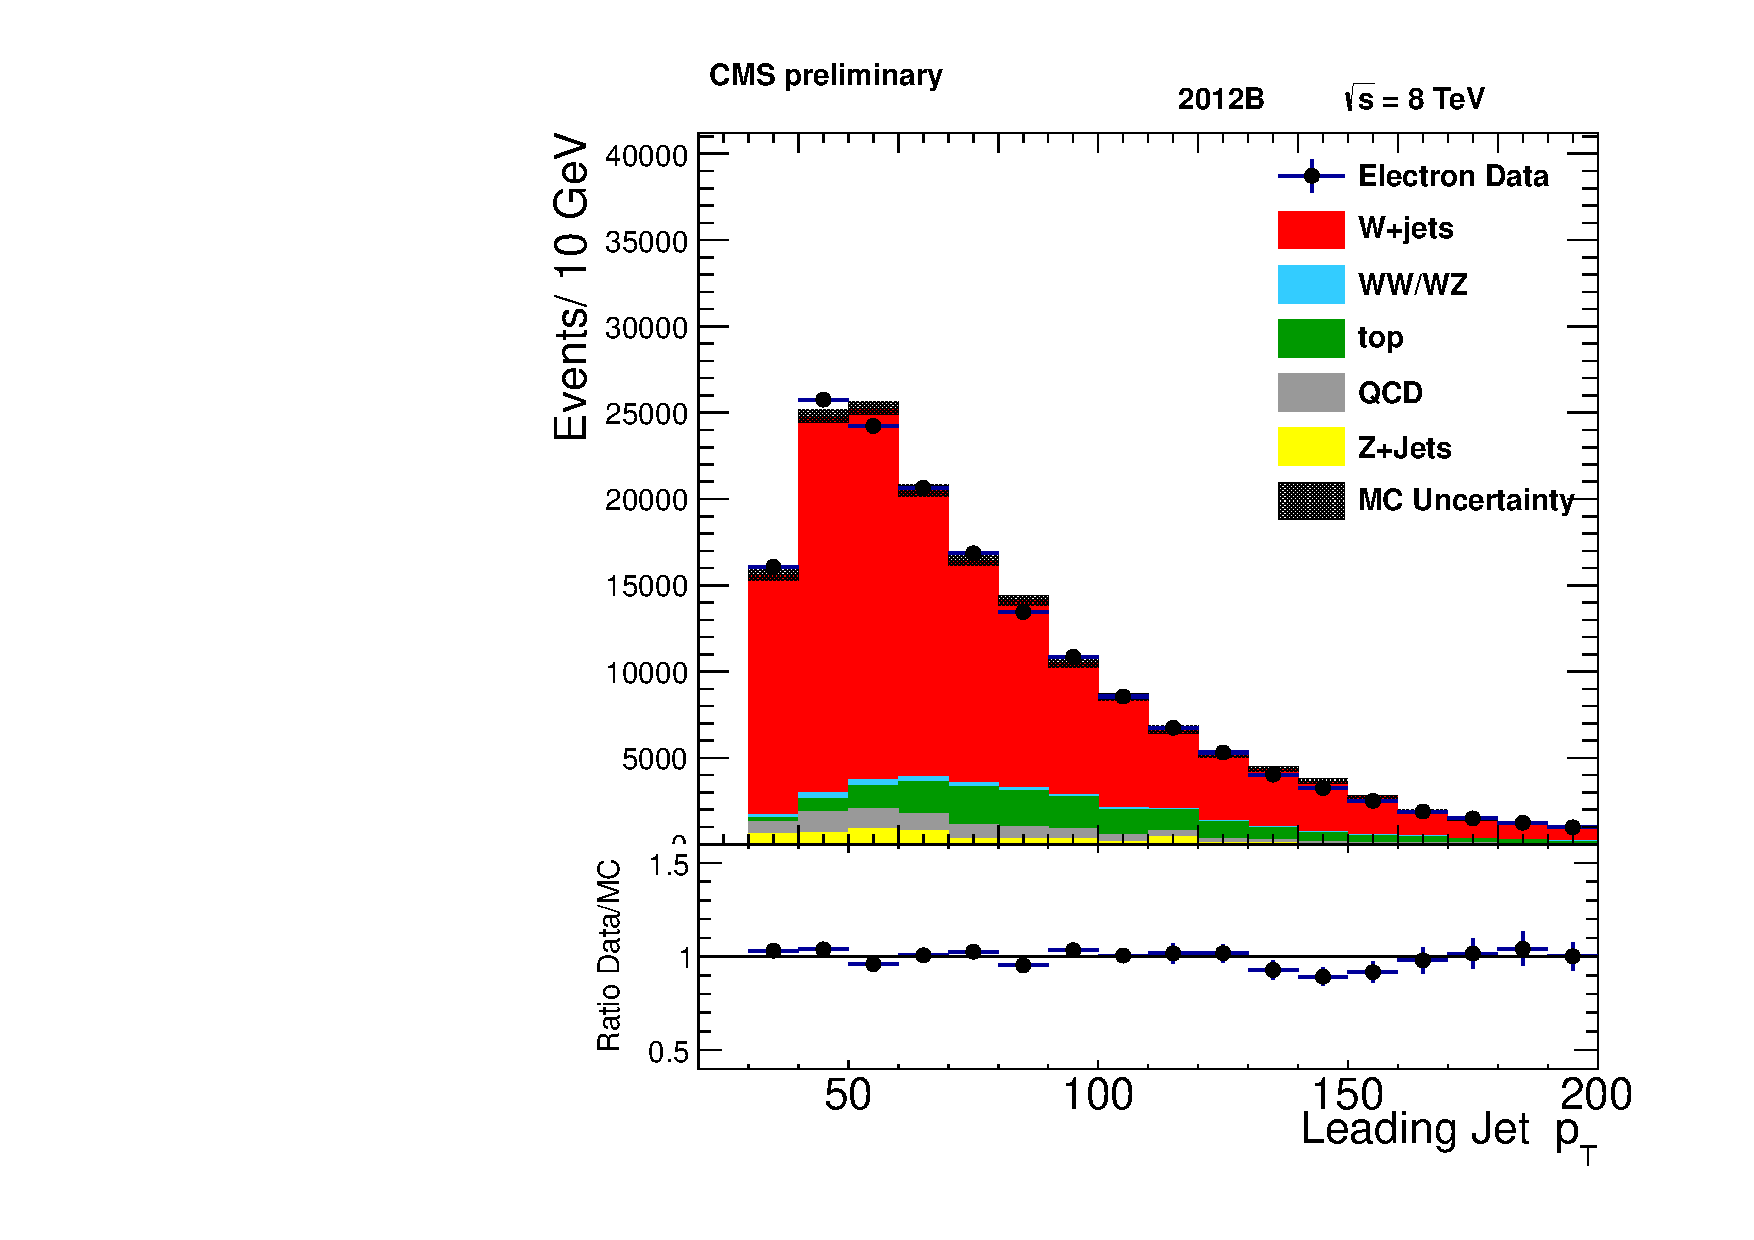
\includegraphics[width=0.3\textwidth]{plots/el_jetld_pt_2012B.pdf}
    }
    \\
    \subfigure[2012A: second jet $p_{T}$]{
      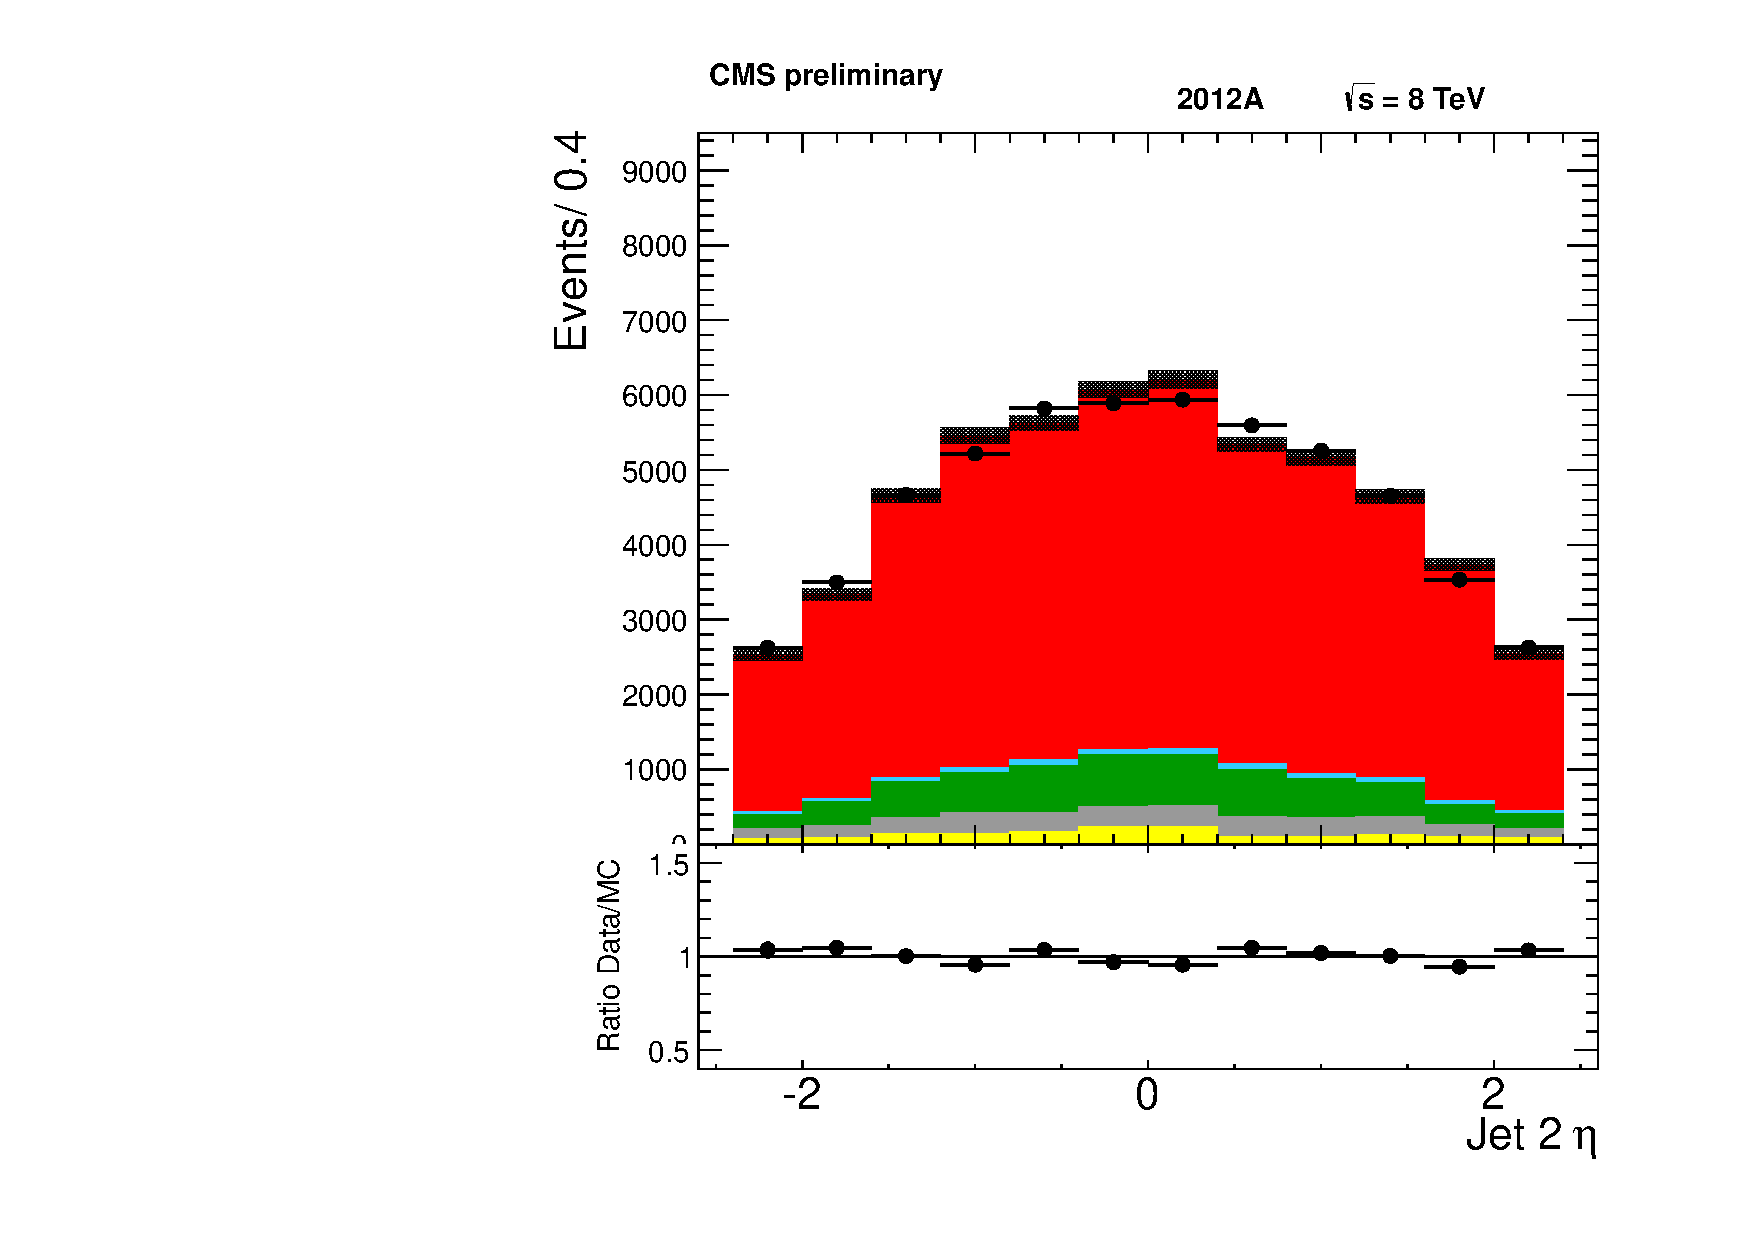
\includegraphics[width=0.3\textwidth]{plots/el_jetnt_eta_2012A.pdf}
    }
    \subfigure[2012B: second jet $p_{T}$]{
      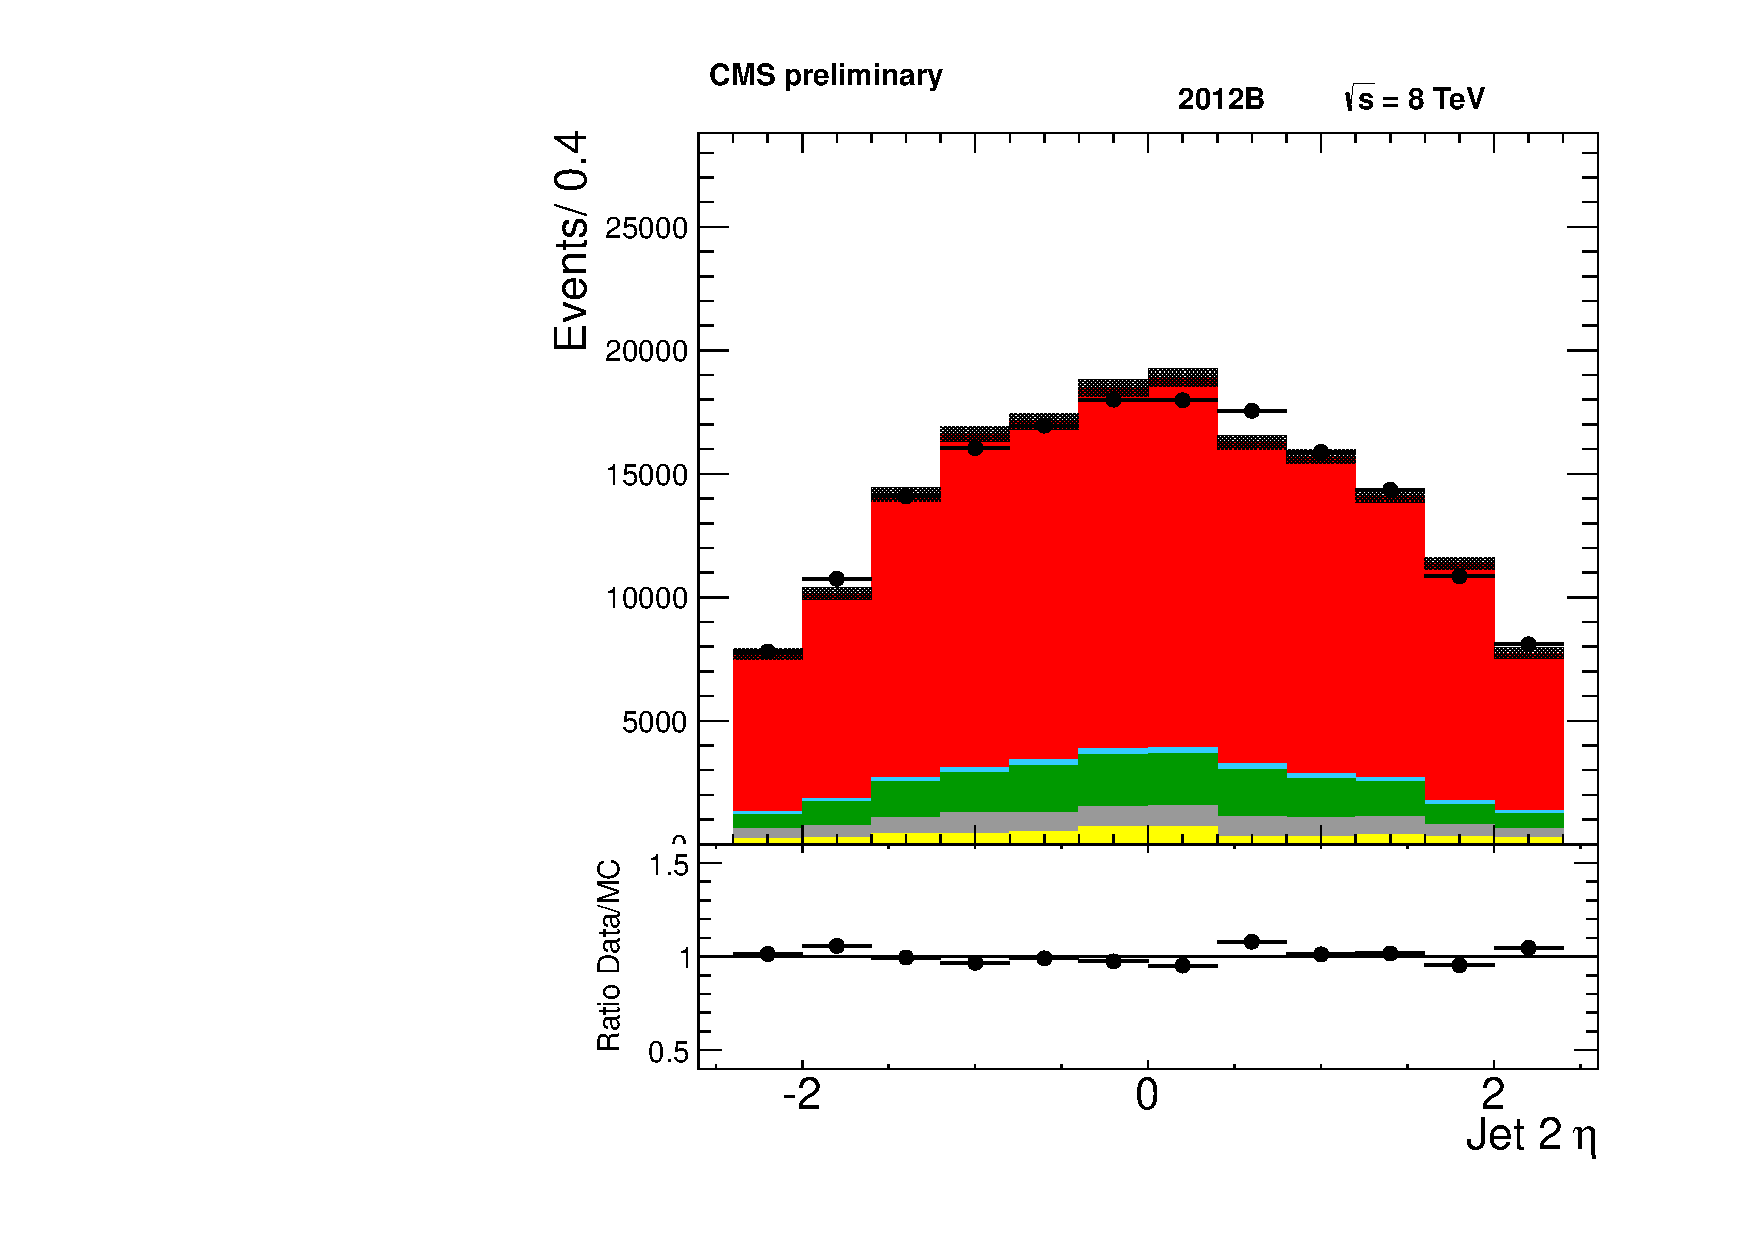
\includegraphics[width=0.3\textwidth]{plots/el_jetnt_eta_2012B.pdf}
    }
    \\
    \subfigure[2012A: leading jet $\eta$]{
      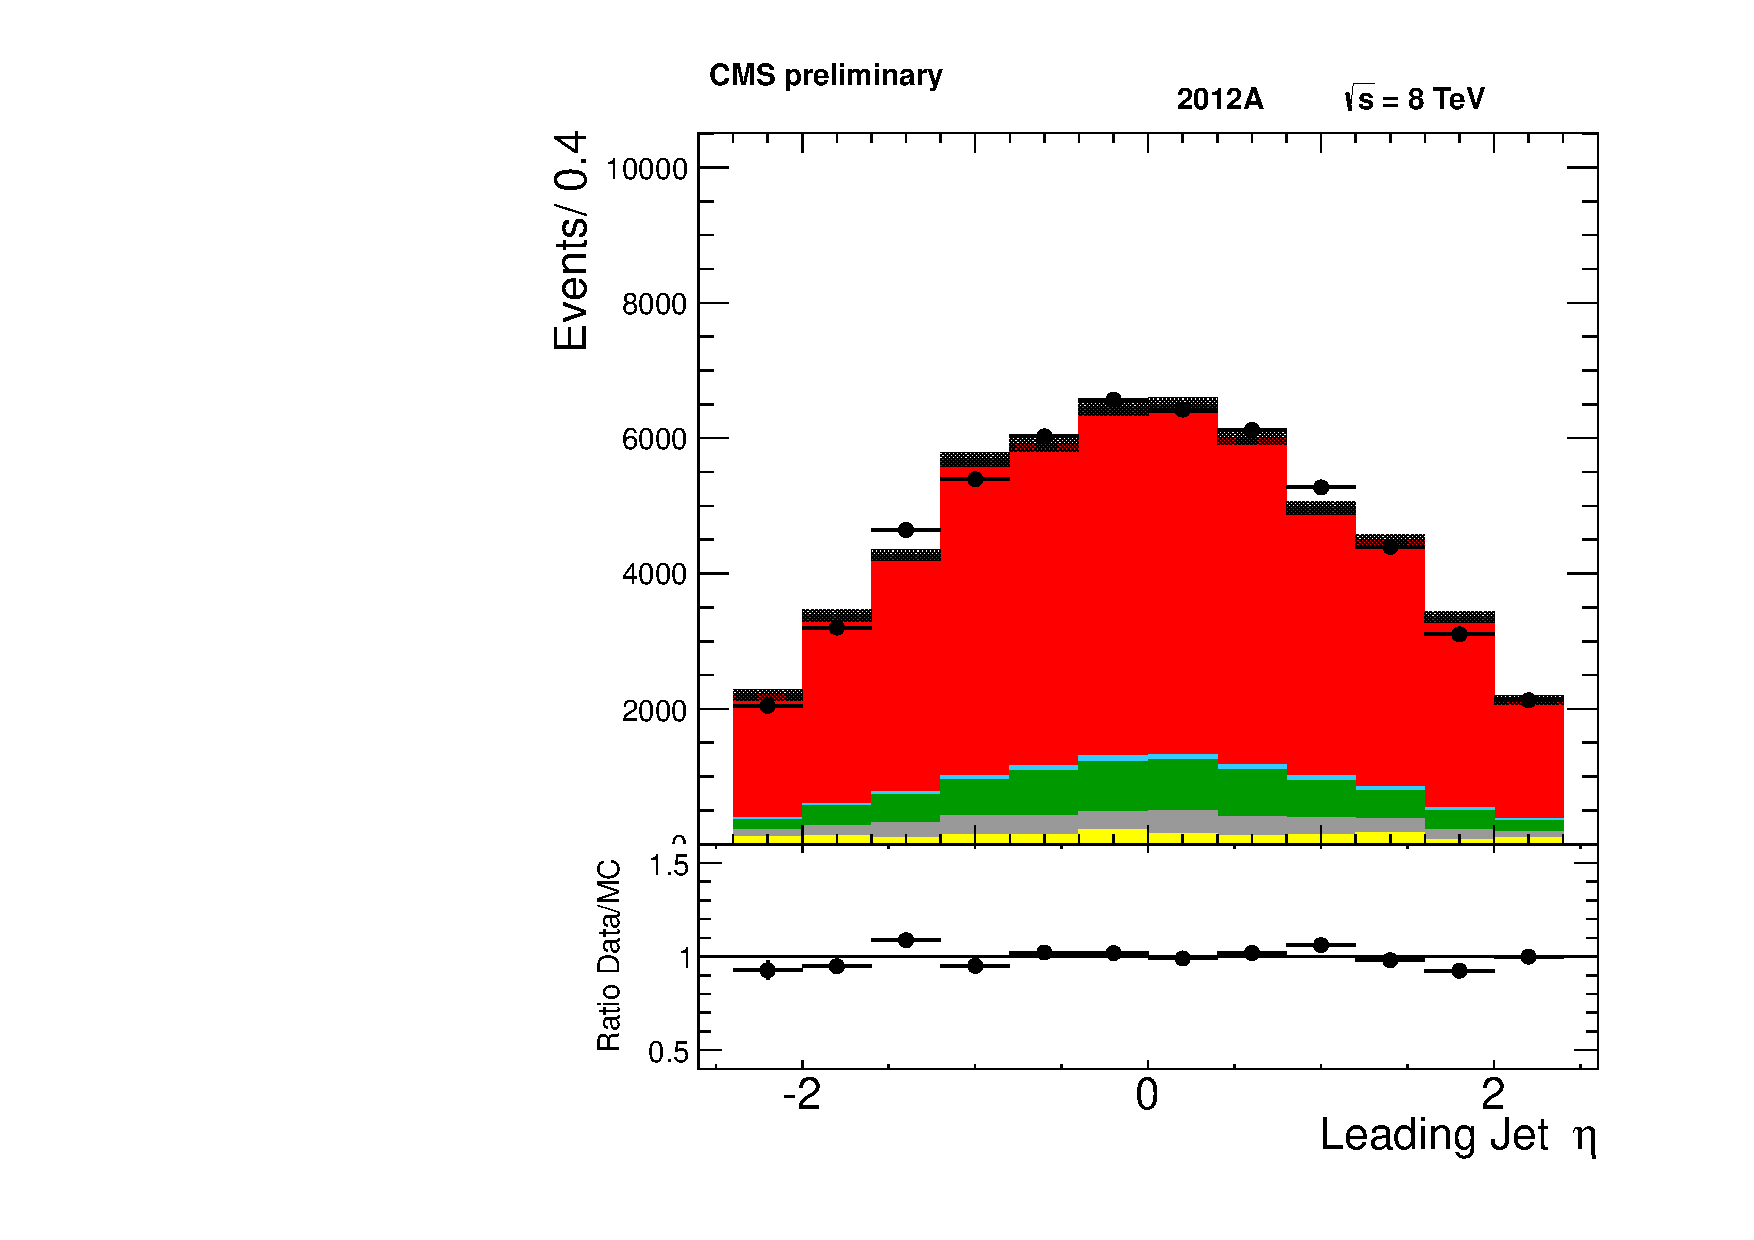
\includegraphics[width=0.3\textwidth]{plots/el_jetld_eta_2012A.pdf}
    }
    \subfigure[2012B: leading jet $\eta$]{
      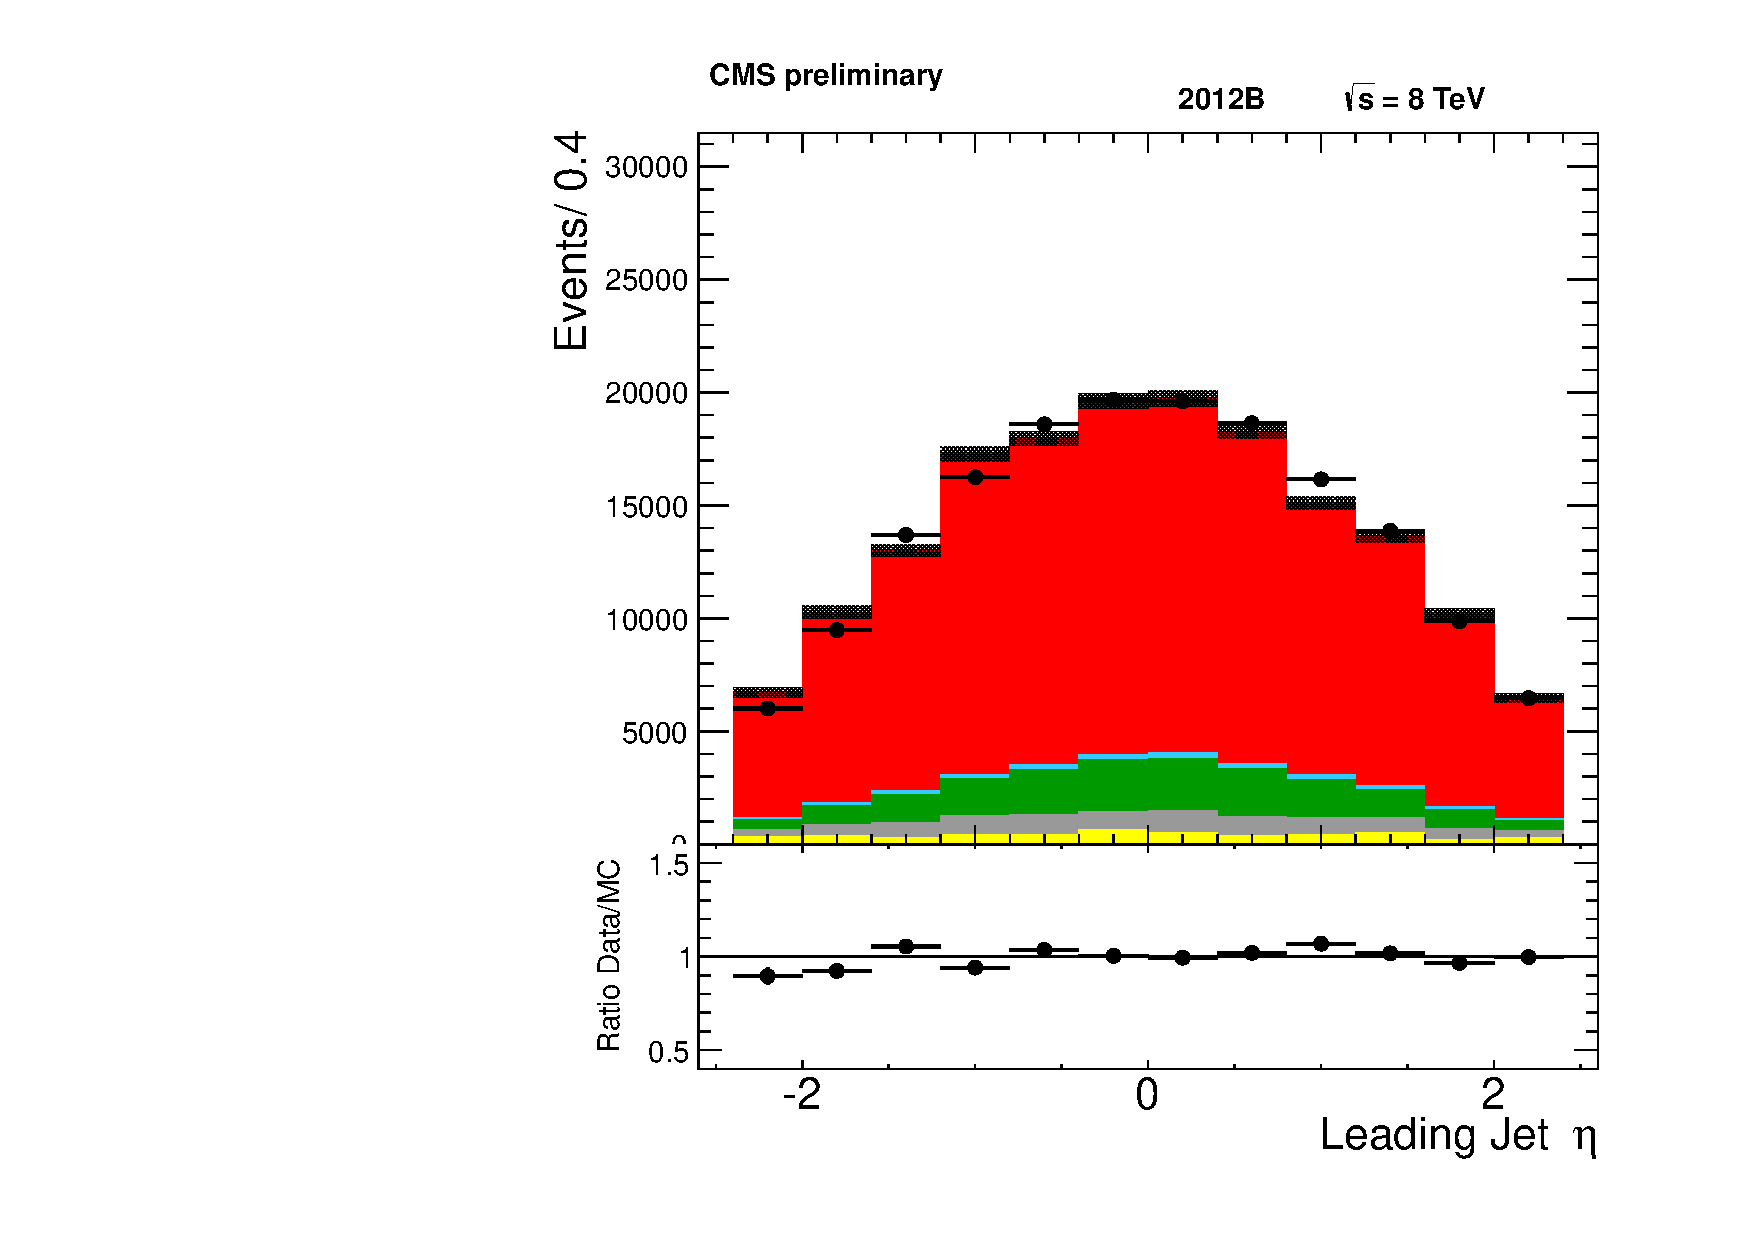
\includegraphics[width=0.3\textwidth]{plots/el_jetld_eta_2012B.pdf}
    }
    \\
    \subfigure[2012A: second jet $\eta$ ]{
      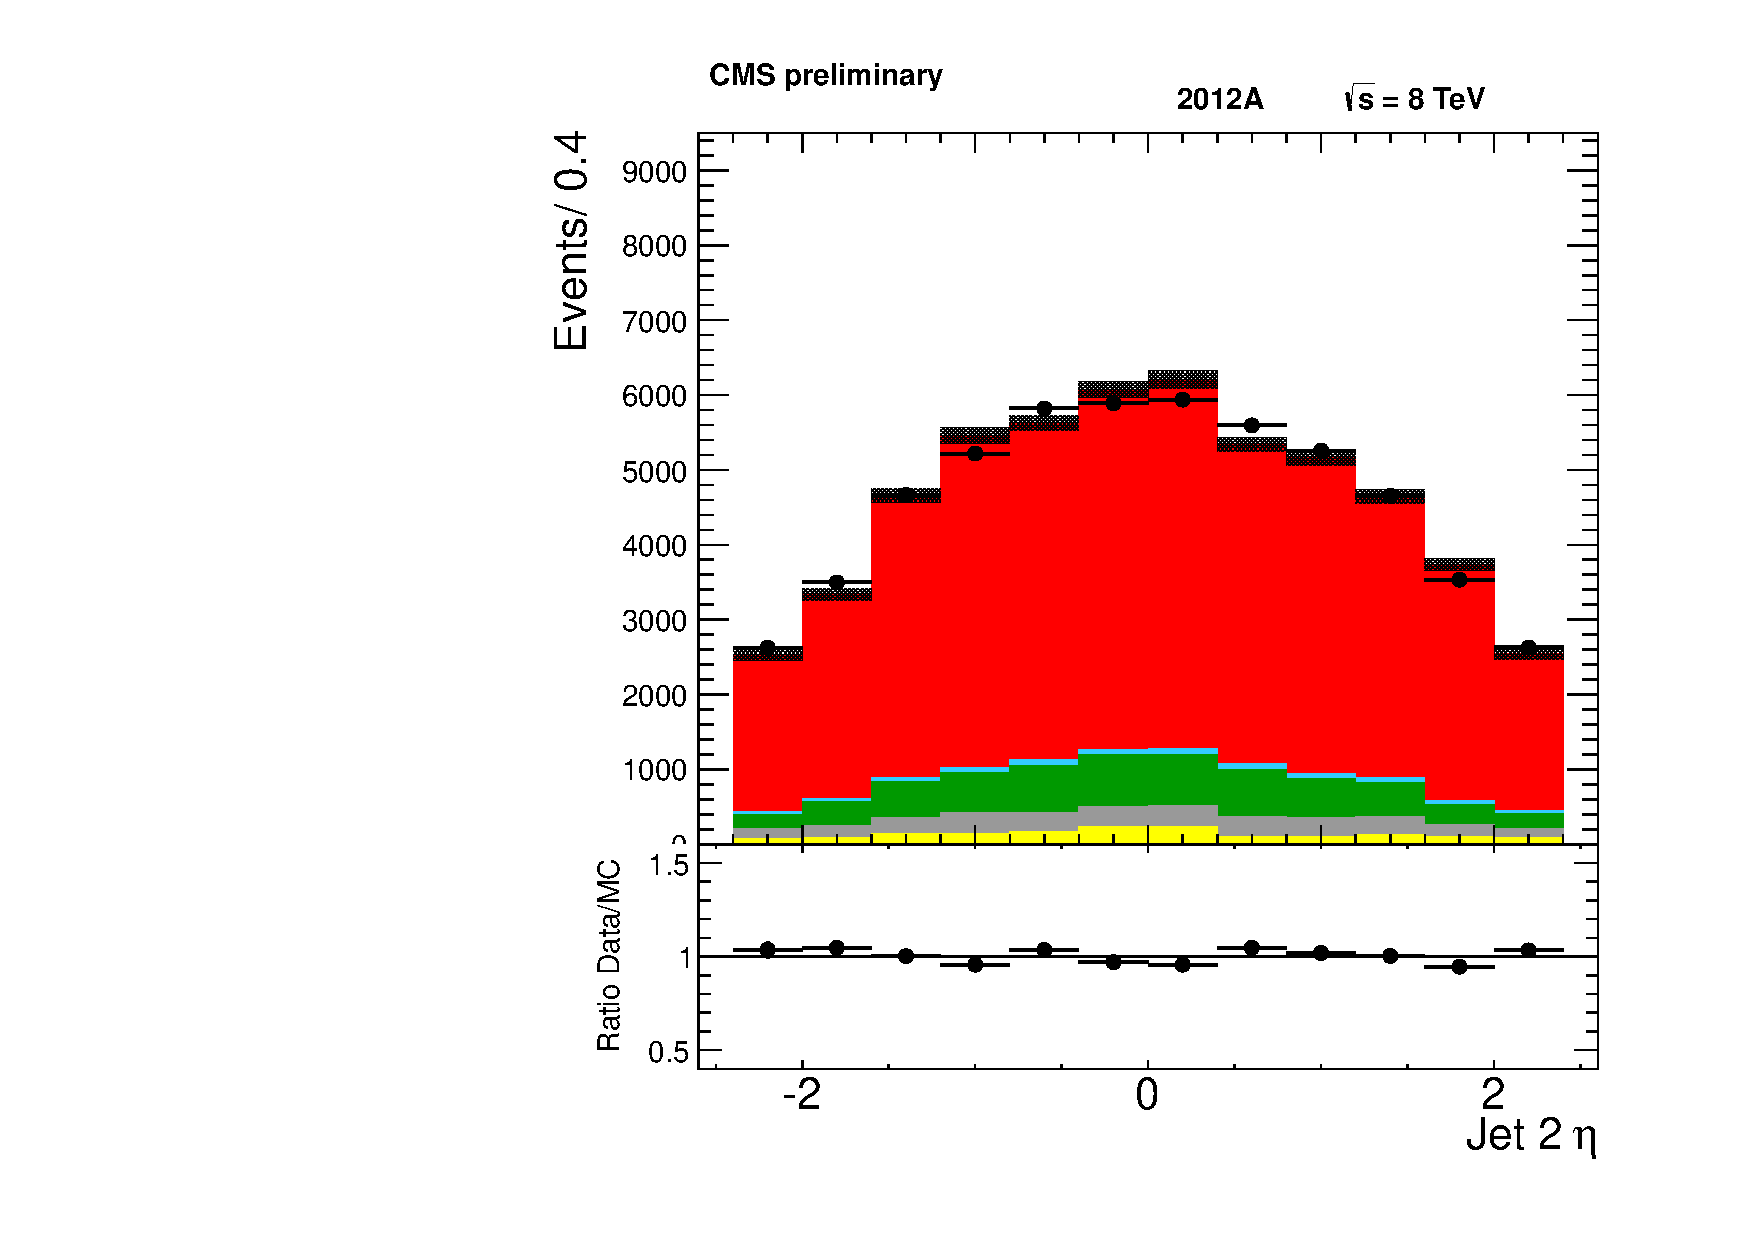
\includegraphics[width=0.3\textwidth]{plots/el_jetnt_eta_2012A.pdf}
    }
    \subfigure[2012B: second jet $\eta$]{
      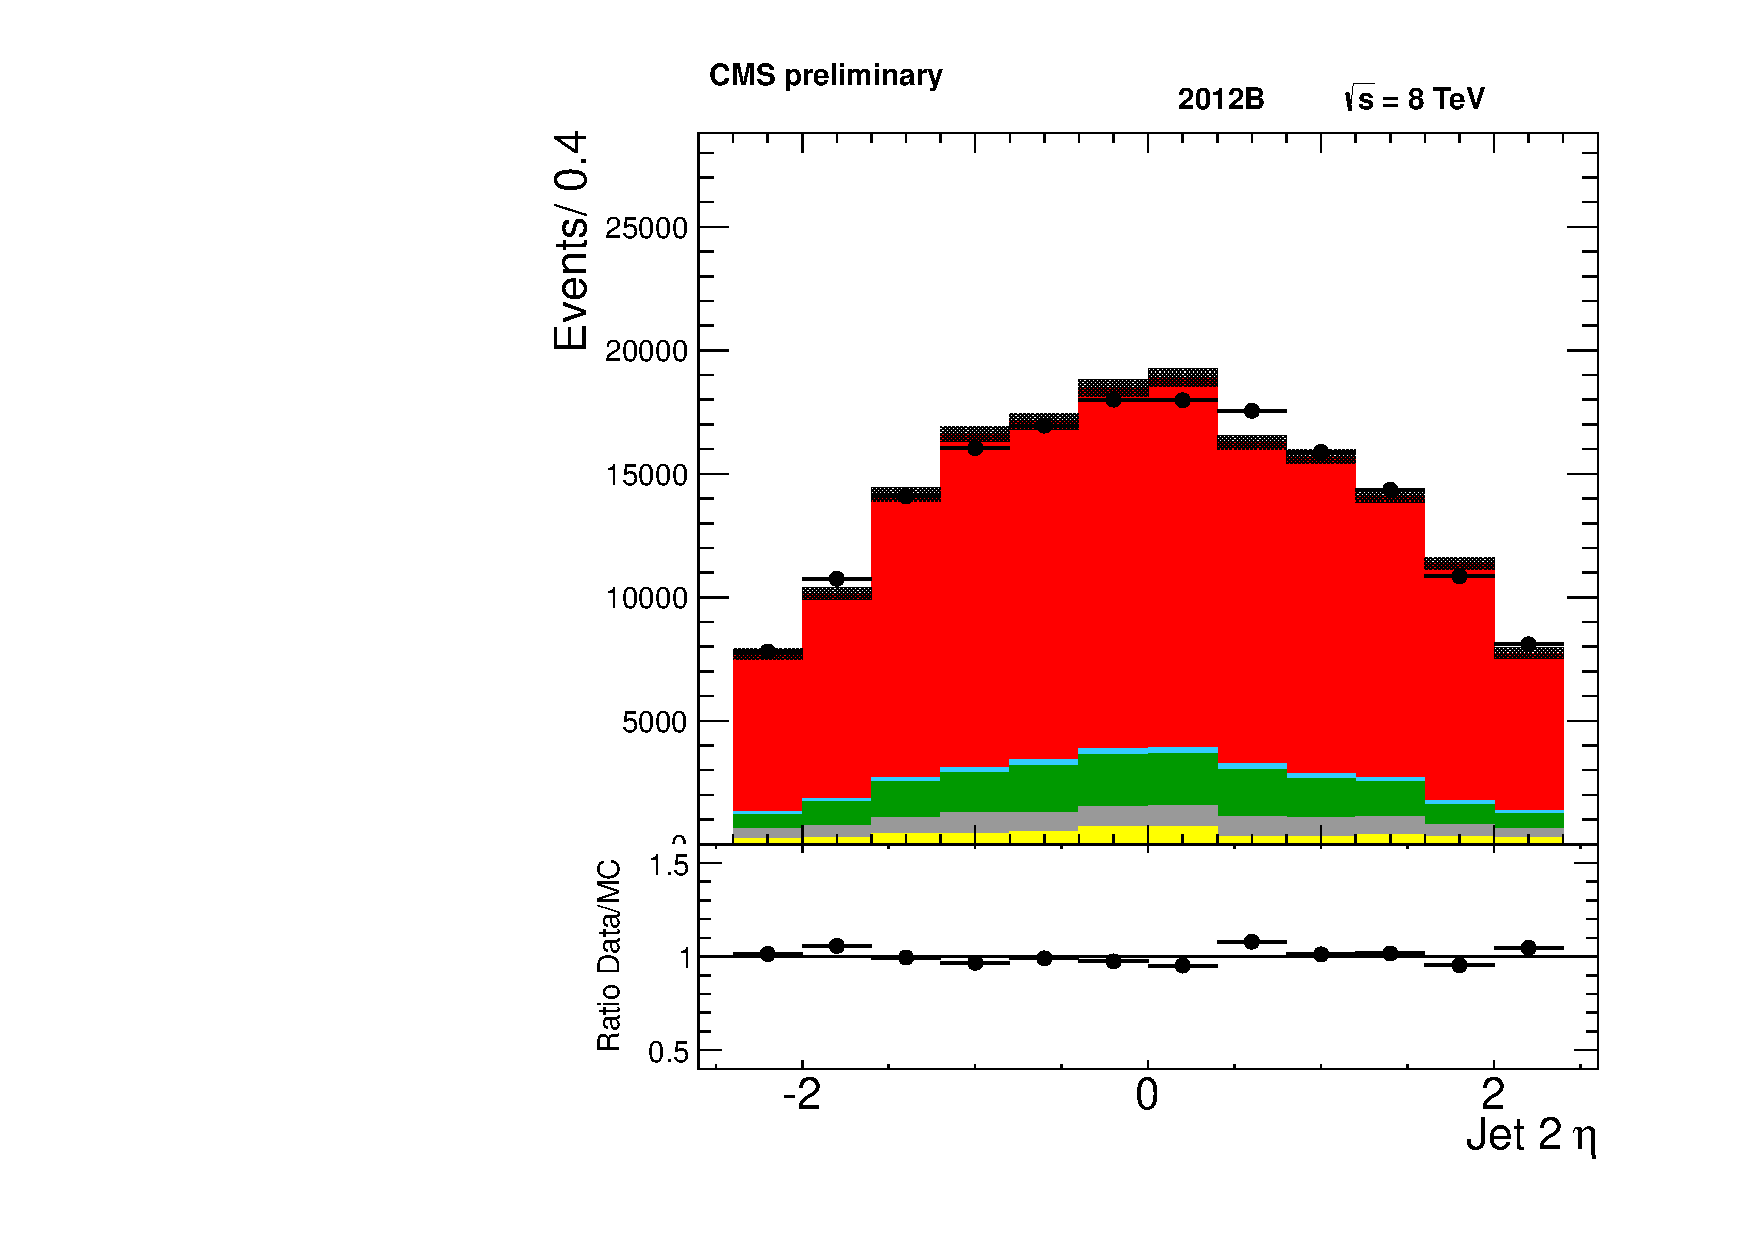
\includegraphics[width=0.3\textwidth]{plots/el_jetnt_eta_2012B.pdf}
    }
    \caption{
             Comparison of the leading jet and second jet $p_{T}$ and $\eta$ distributions from data and MC for the electron+jets
      selection.
            }
    \label{fig:CP2012AB4}
\end{figure}


\begin{figure}[htb]
  \centering
    \subfigure[2012A: electron $p_{T}$]{
      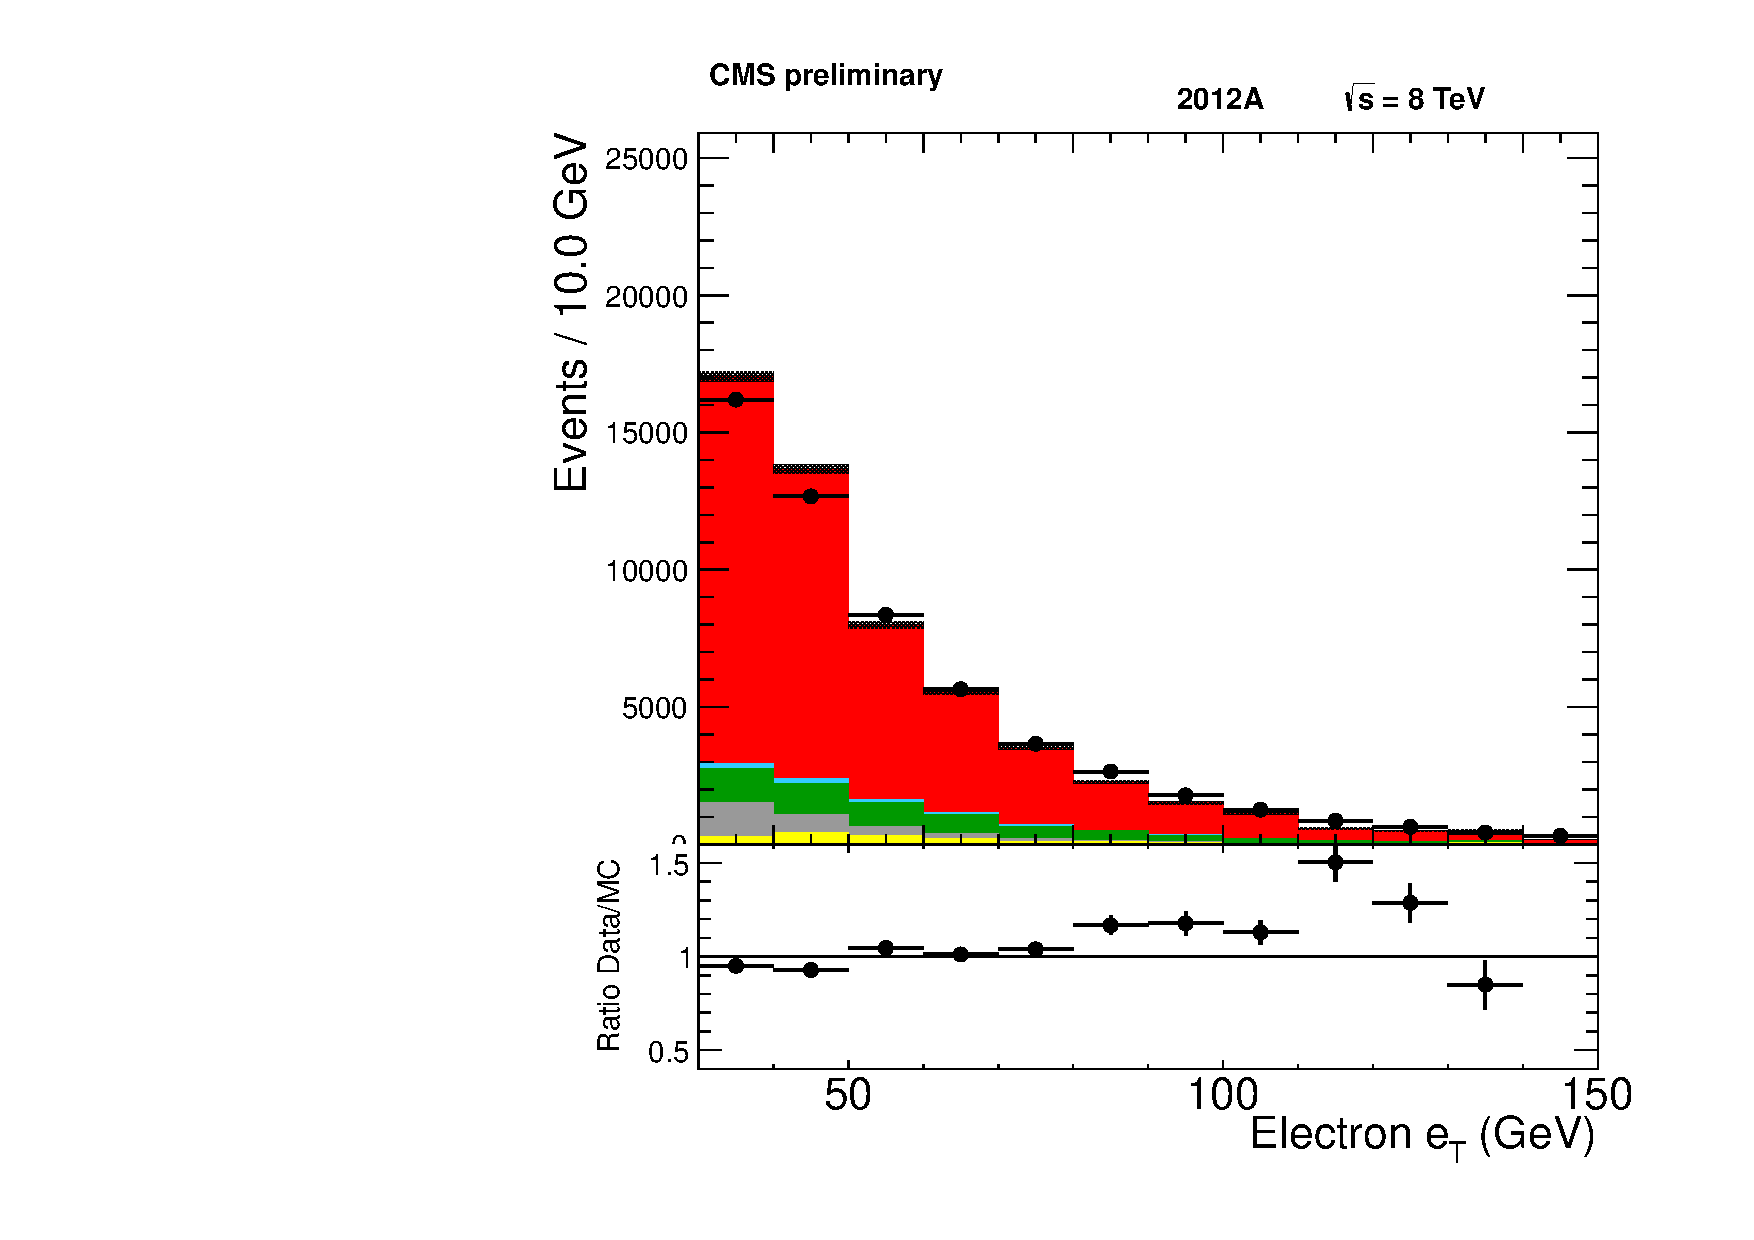
\includegraphics[width=0.4\textwidth]{plots/el_W_electron_et_2012A.pdf}
    }
    \subfigure[2012B: electron $p_{T}$]{
      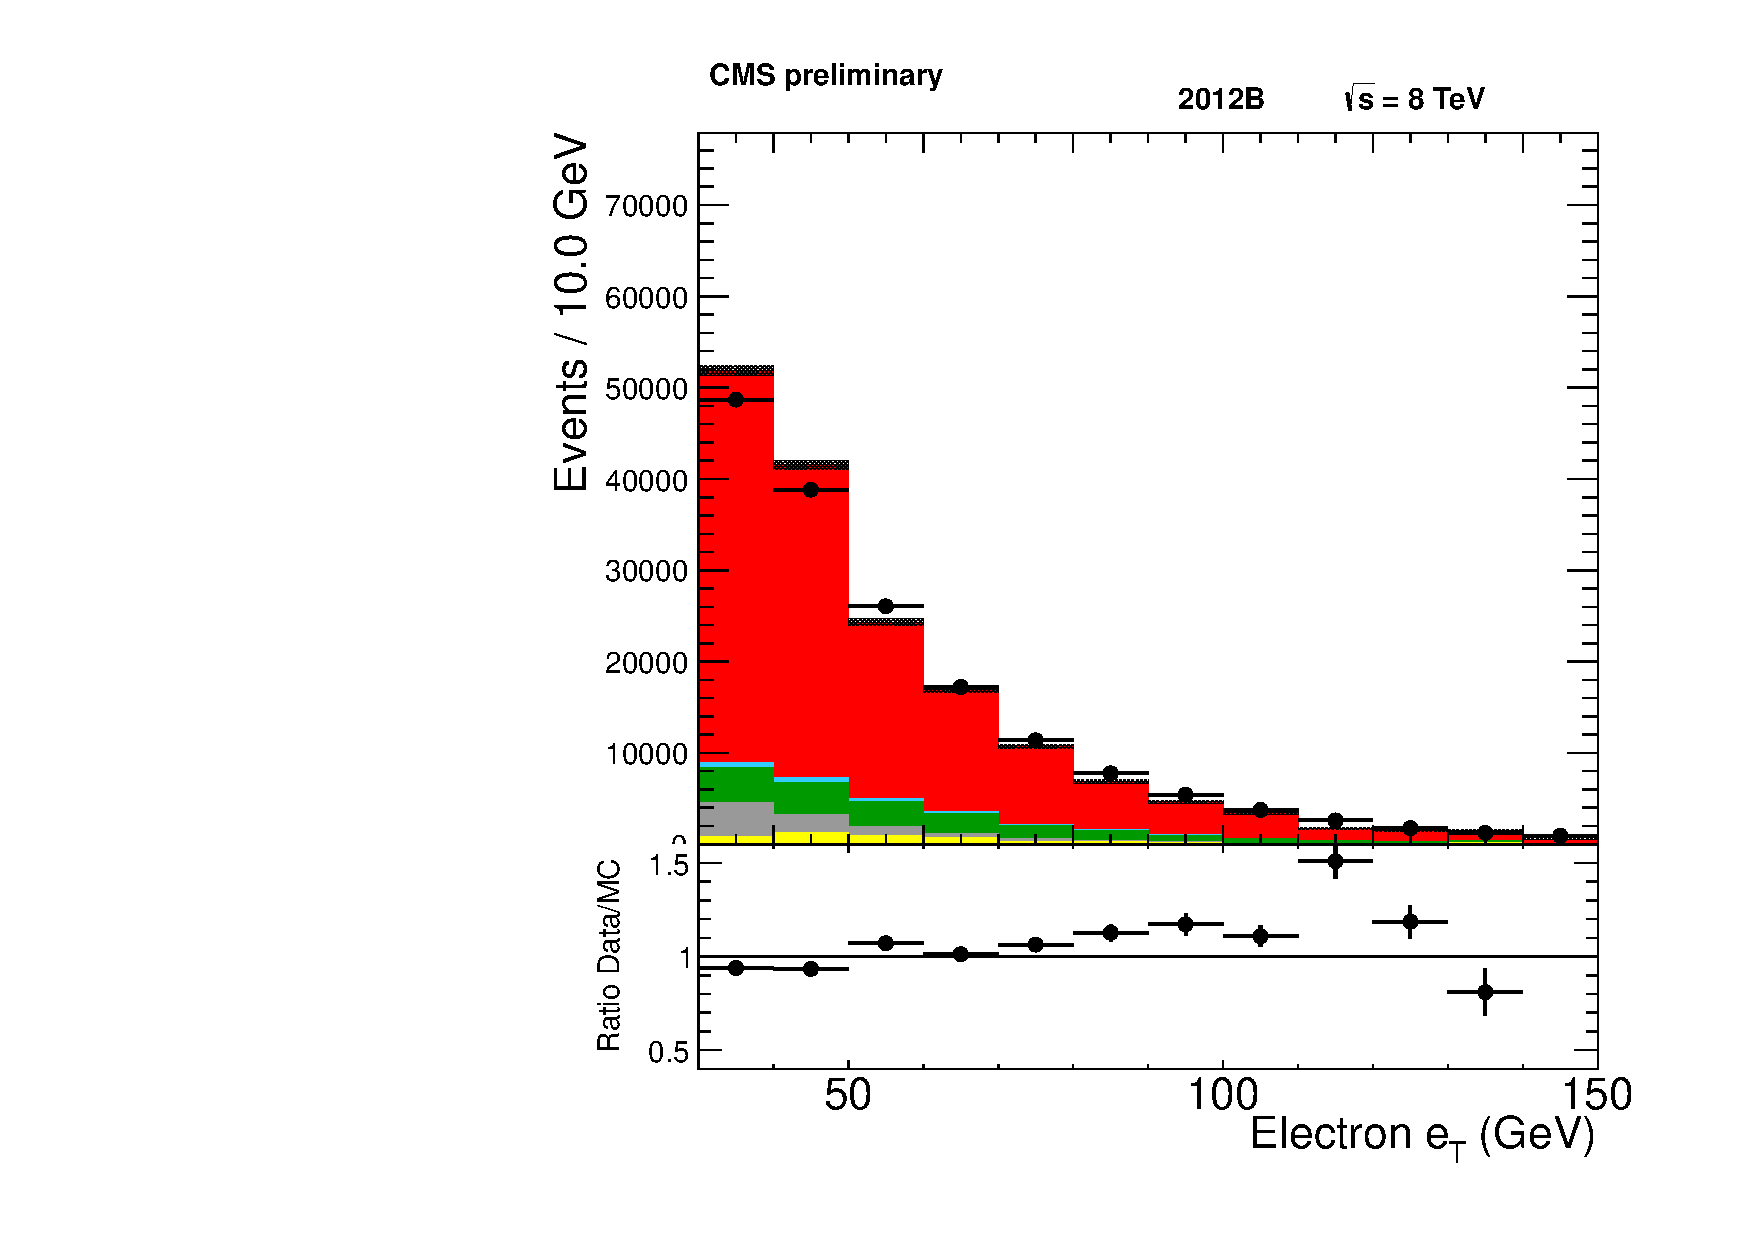
\includegraphics[width=0.4\textwidth]{plots/el_W_electron_et_2012B.pdf}
    }
    \\
    \subfigure[2012A: electron $\eta$]{
      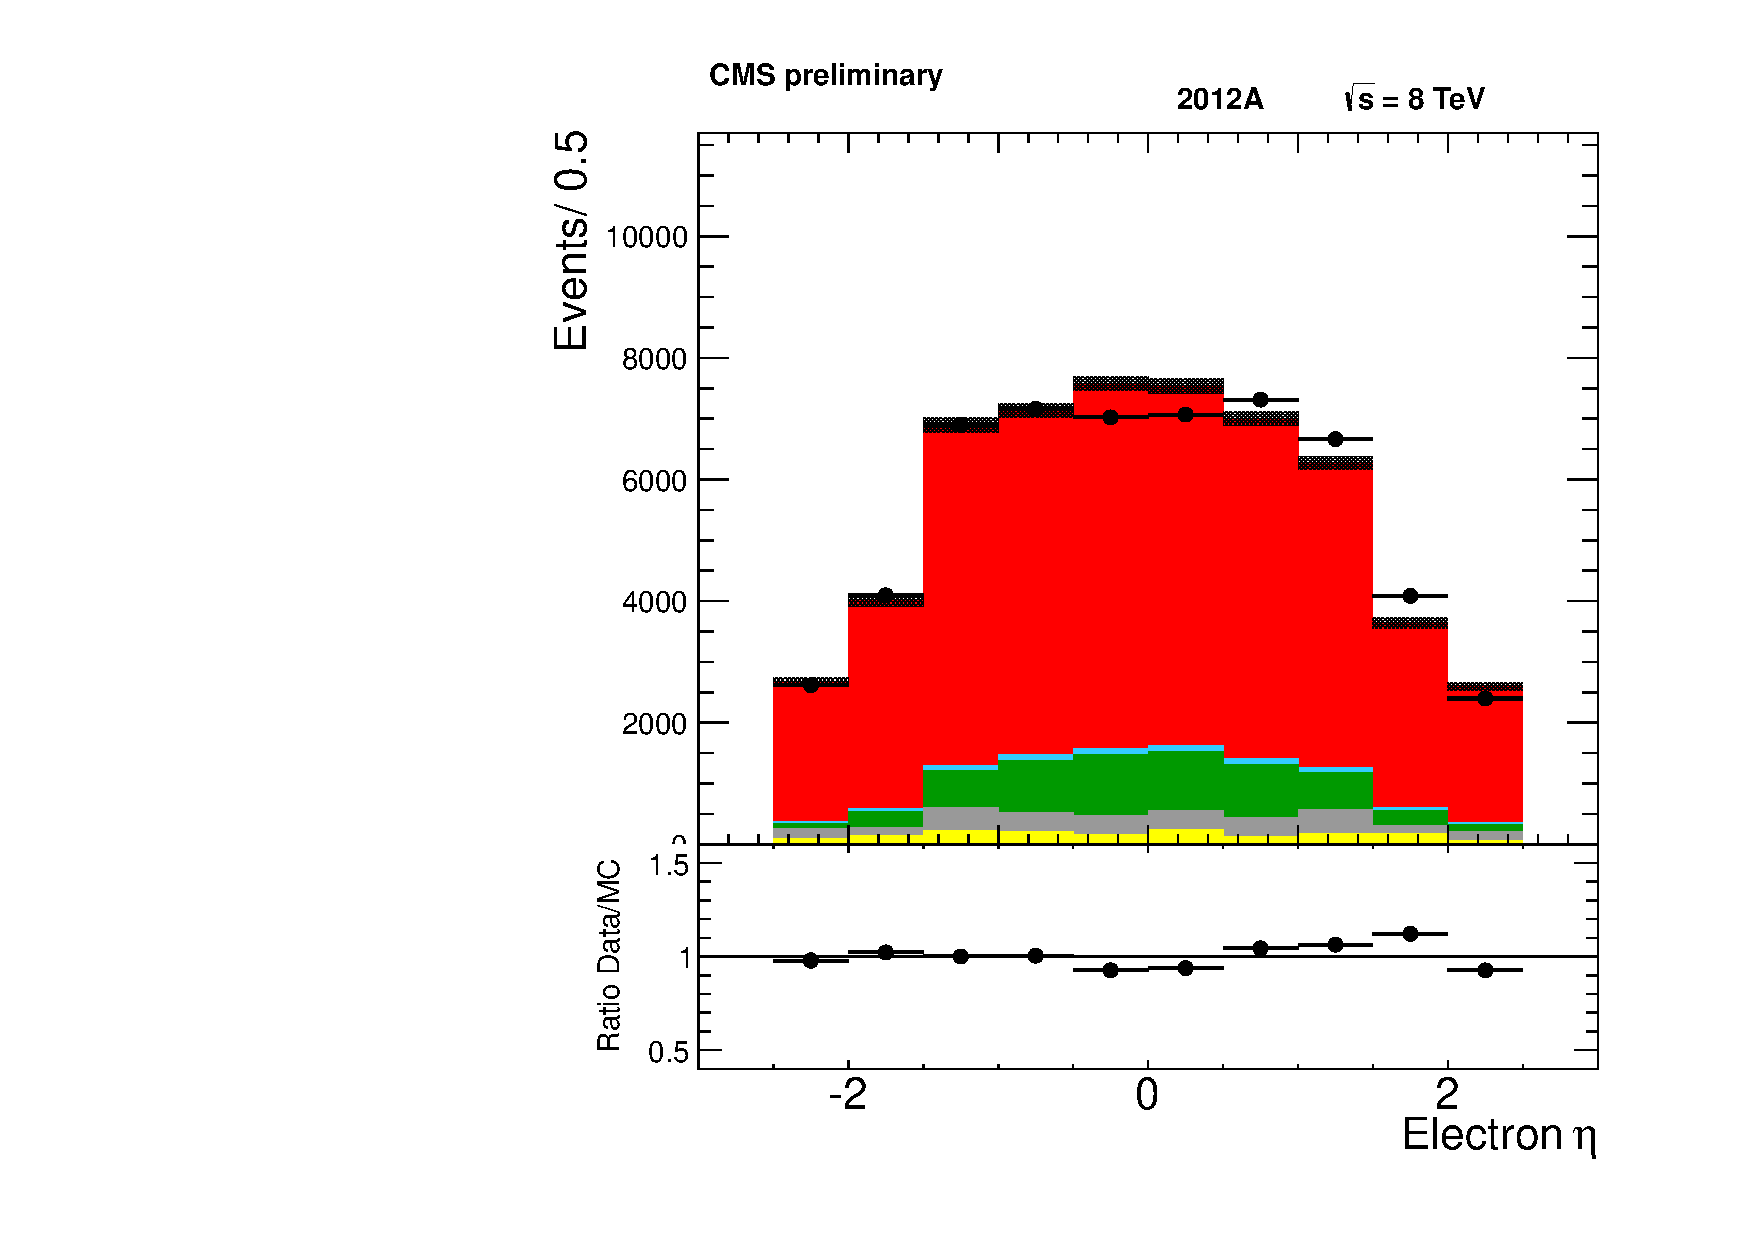
\includegraphics[width=0.4\textwidth]{plots/el_W_electron_eta_2012A.pdf}
    }
    \subfigure[2012B: electron $\eta$]{
      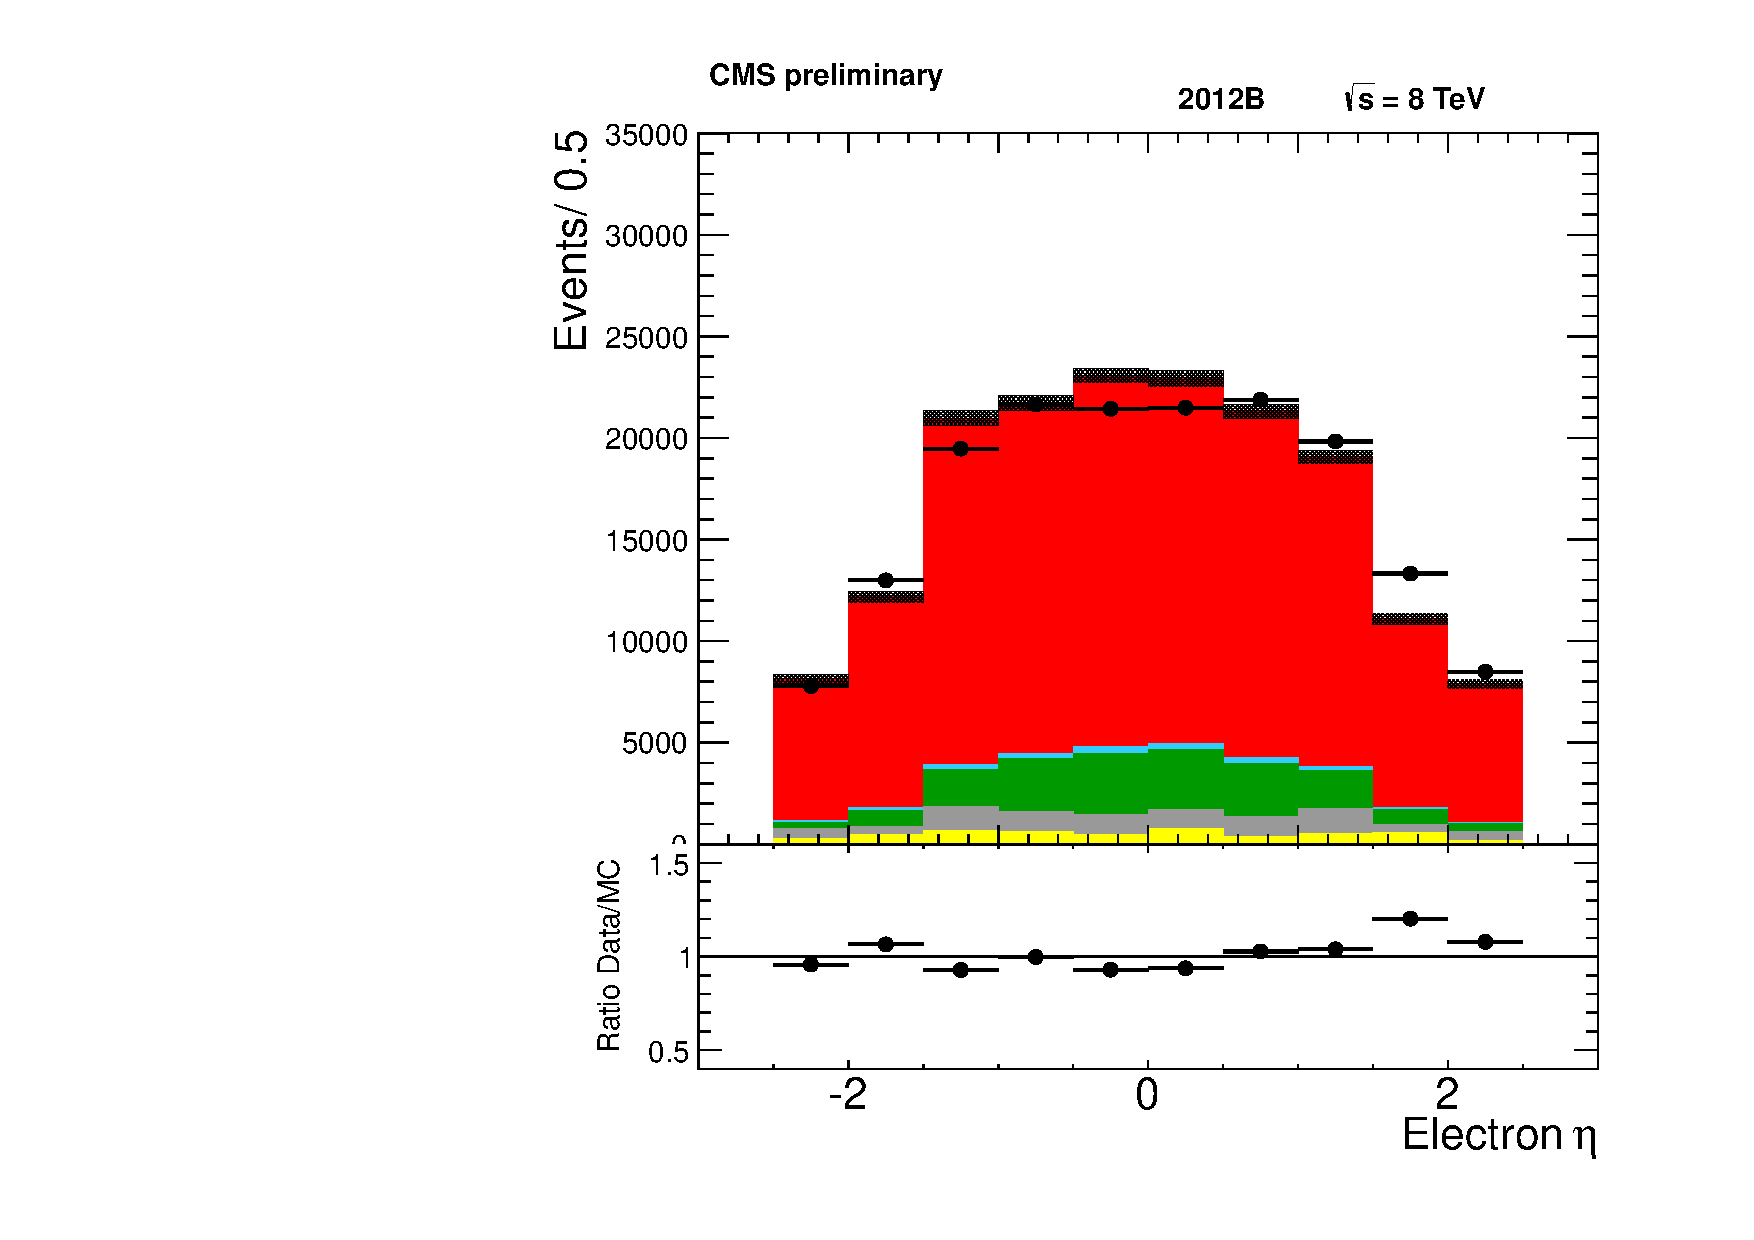
\includegraphics[width=0.4\textwidth]{plots/el_W_electron_eta_2012B.pdf}
    }
    \\
    \subfigure[2012A: $M_{T}$]{
      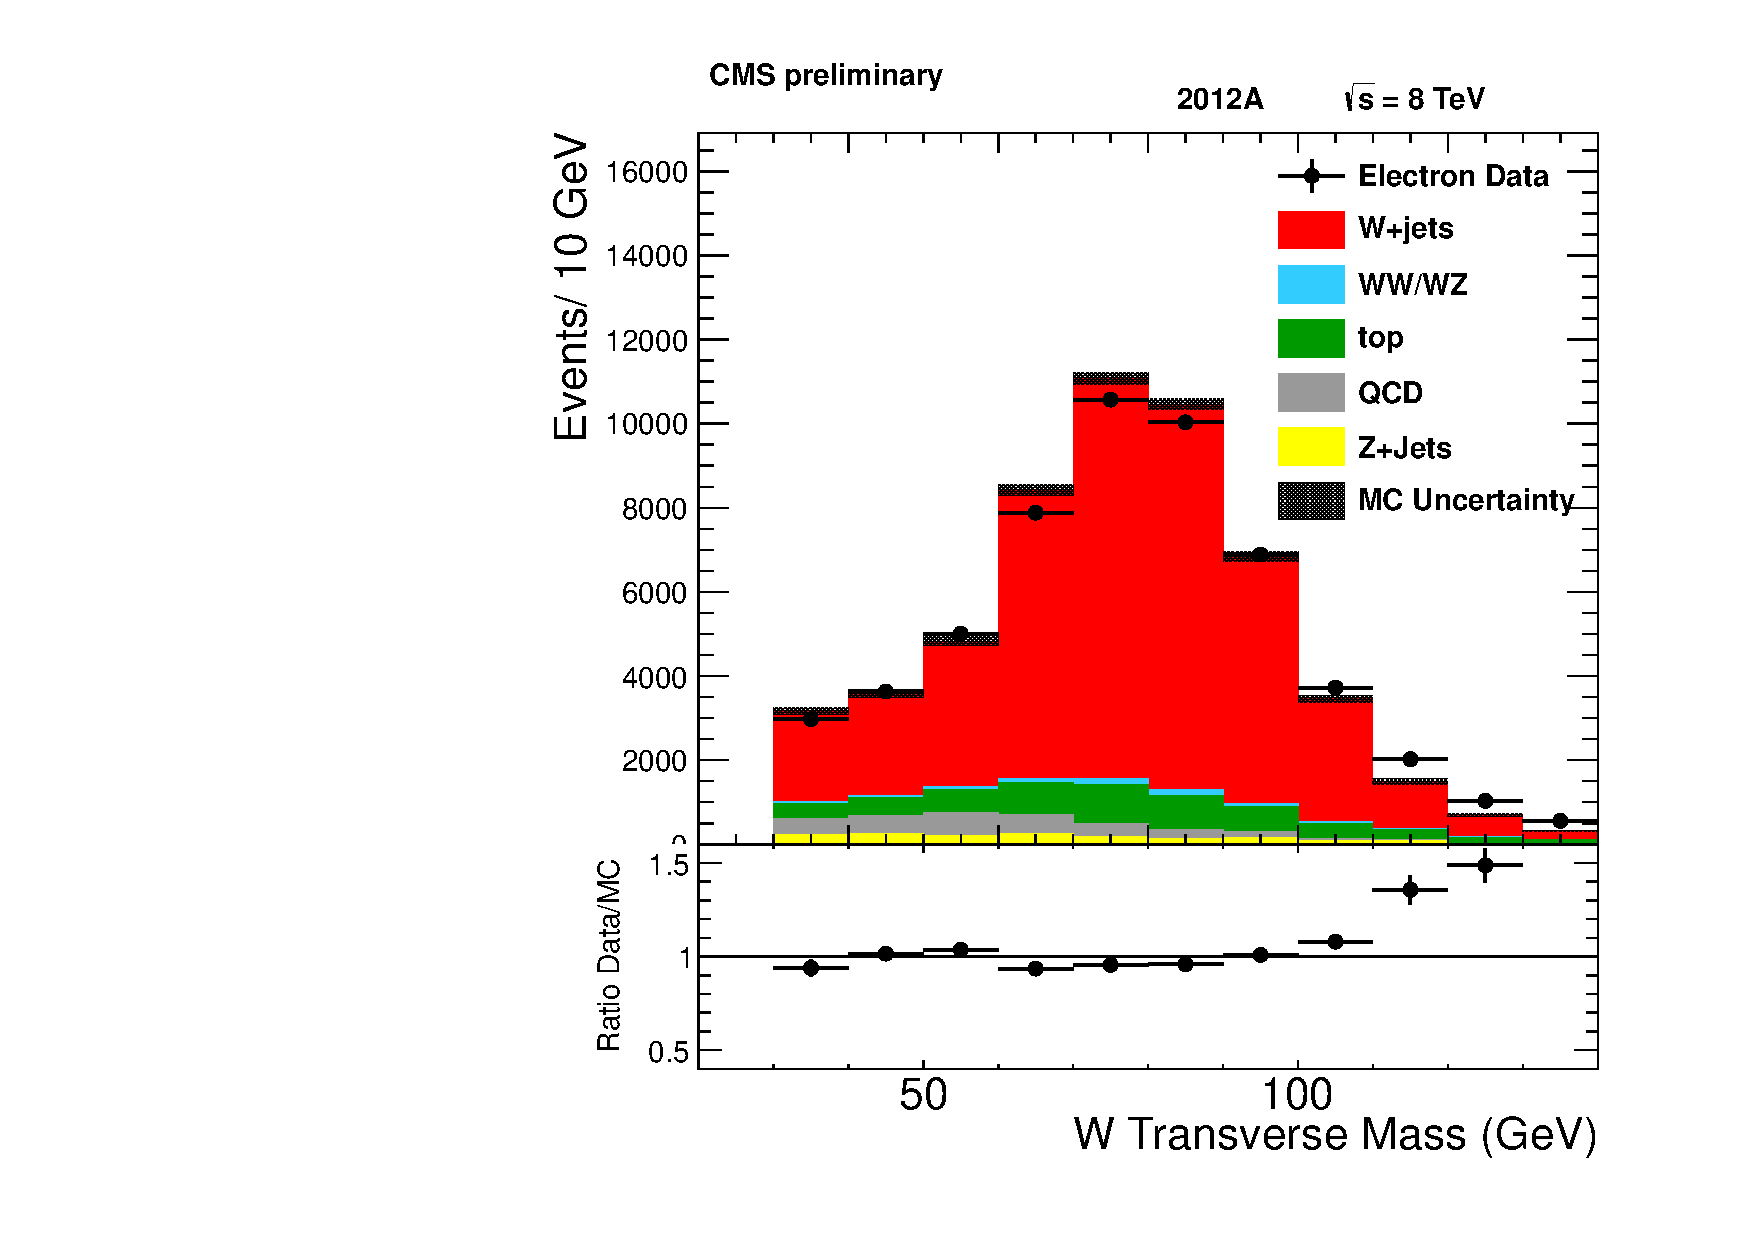
\includegraphics[width=0.4\textwidth]{plots/el_W_mt_2012A.pdf}
    }
    \subfigure[2012B: $M_{T}$]{
      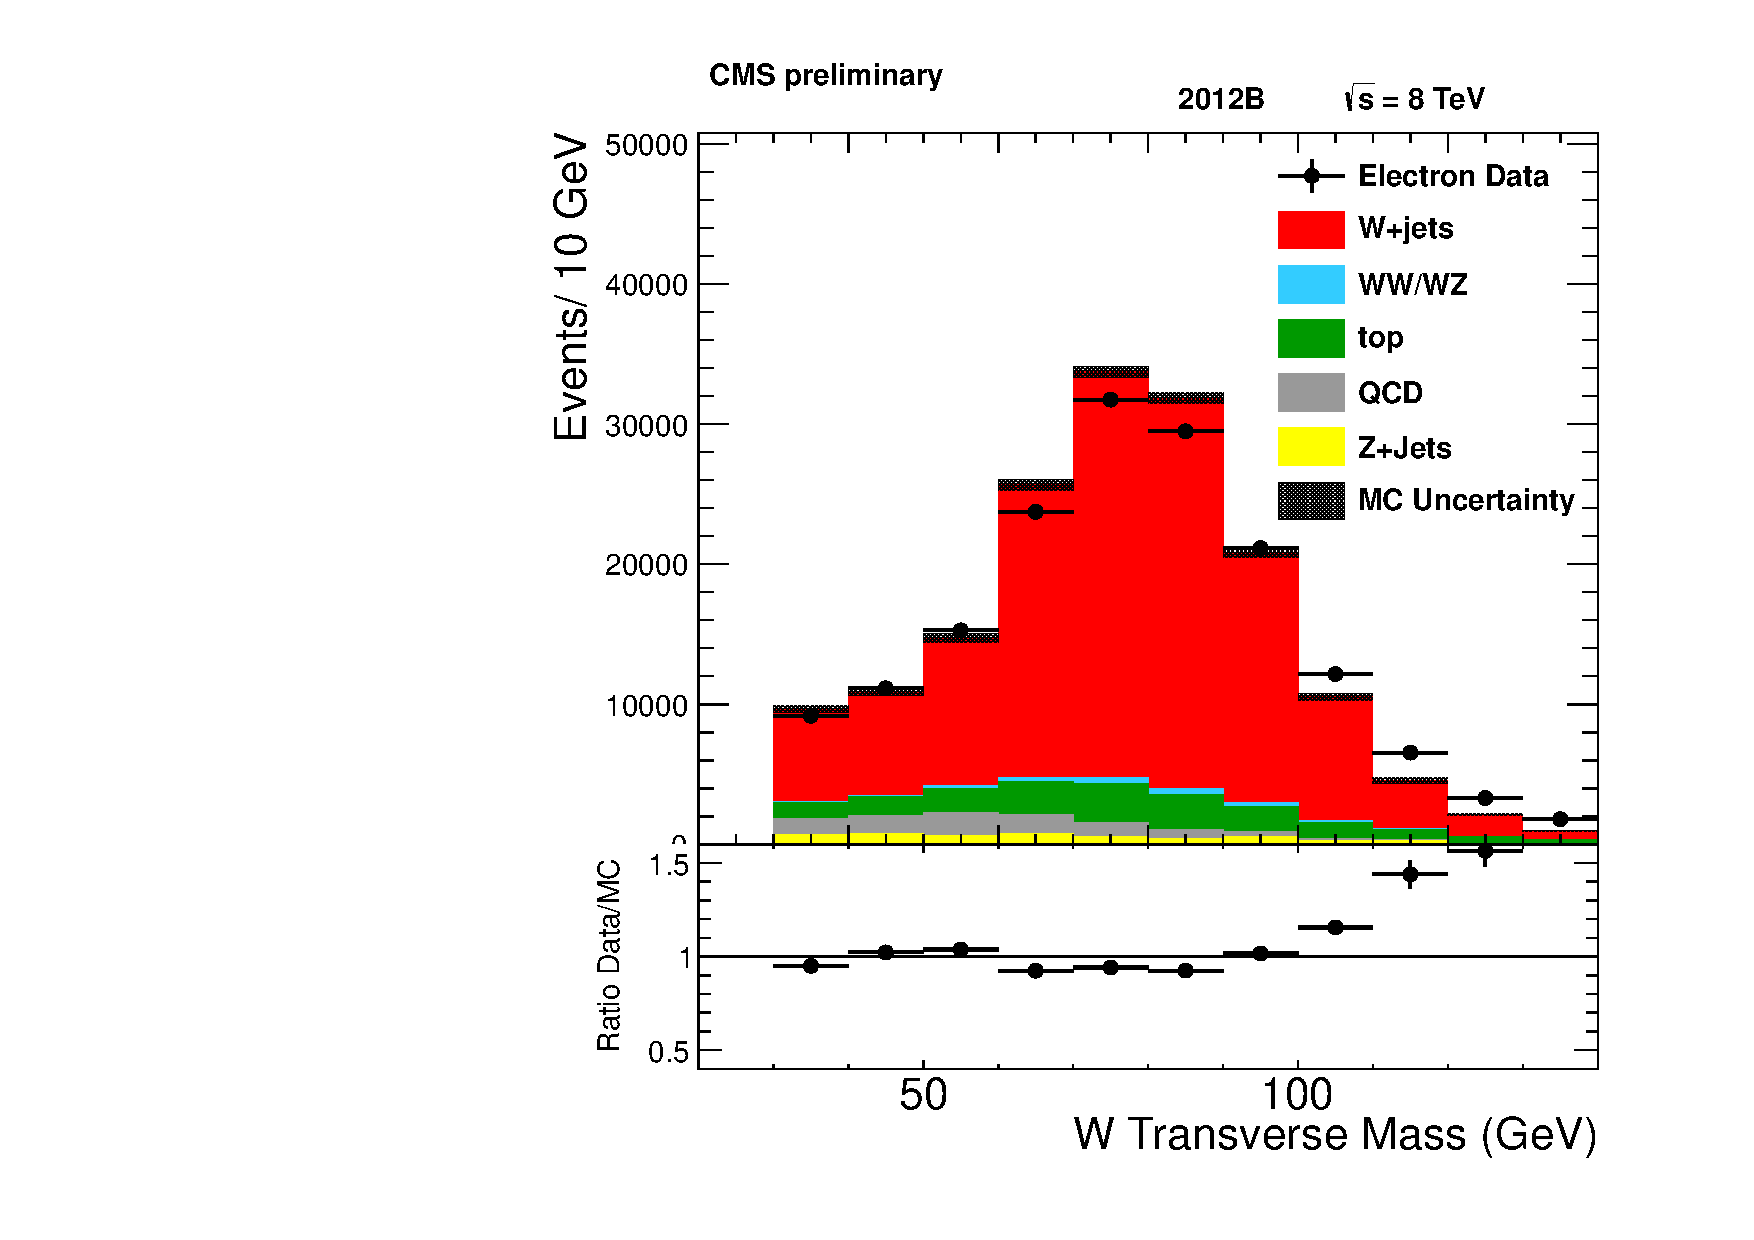
\includegraphics[width=0.4\textwidth]{plots/el_W_mt_2012B.pdf}
    }
    \\
    \caption{
             Comparison of the electron $p_{T}$, $\eta$ and the transverse mass of the electron / MET system distributions from data and MC for 
the electron+jets selection.
            }
    \label{fig:CP2012AB5}
\end{figure}

\begin{figure}[htb]
  \centering
    \subfigure[2012A: MET]{
      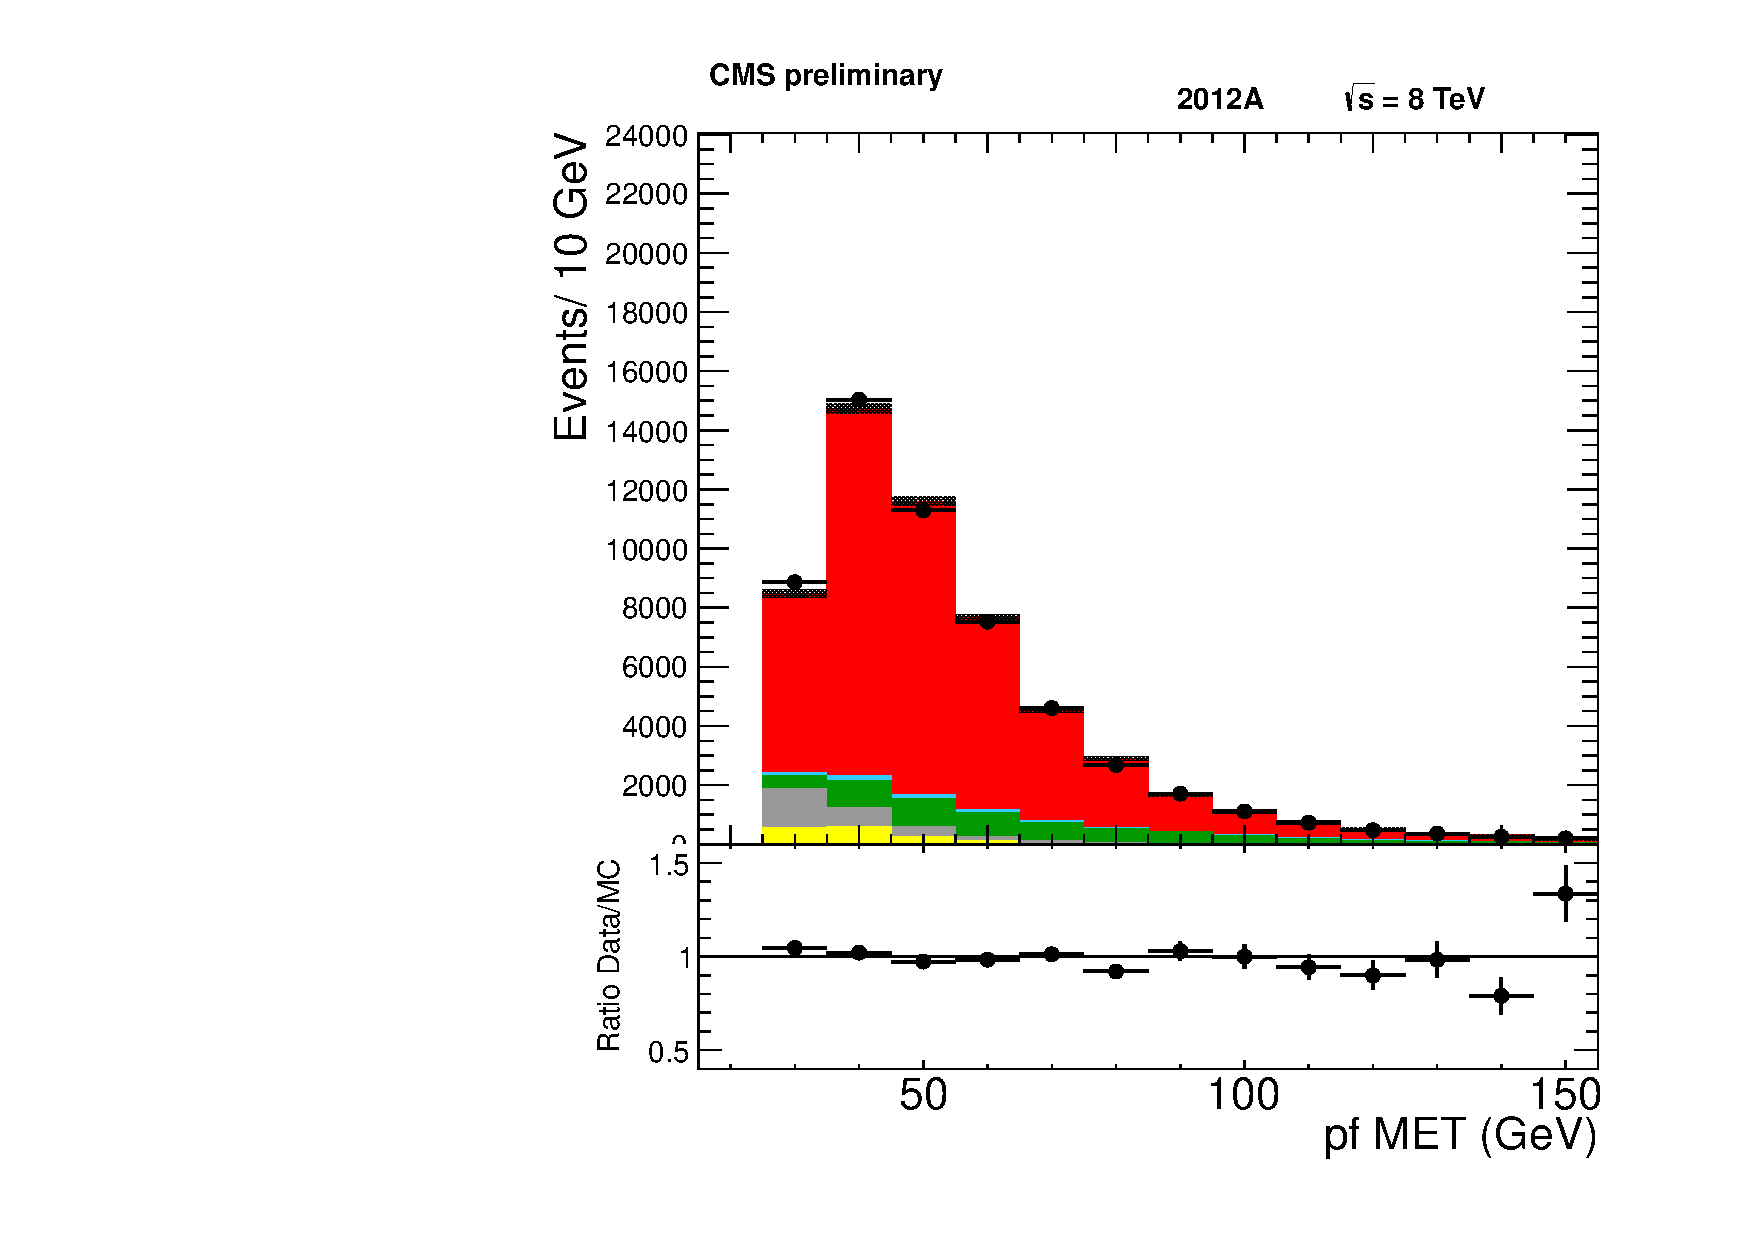
\includegraphics[width=0.4\textwidth]{plots/el_event_met_pfmet_2012A.pdf}
    }
    \subfigure[2012B: MET]{
      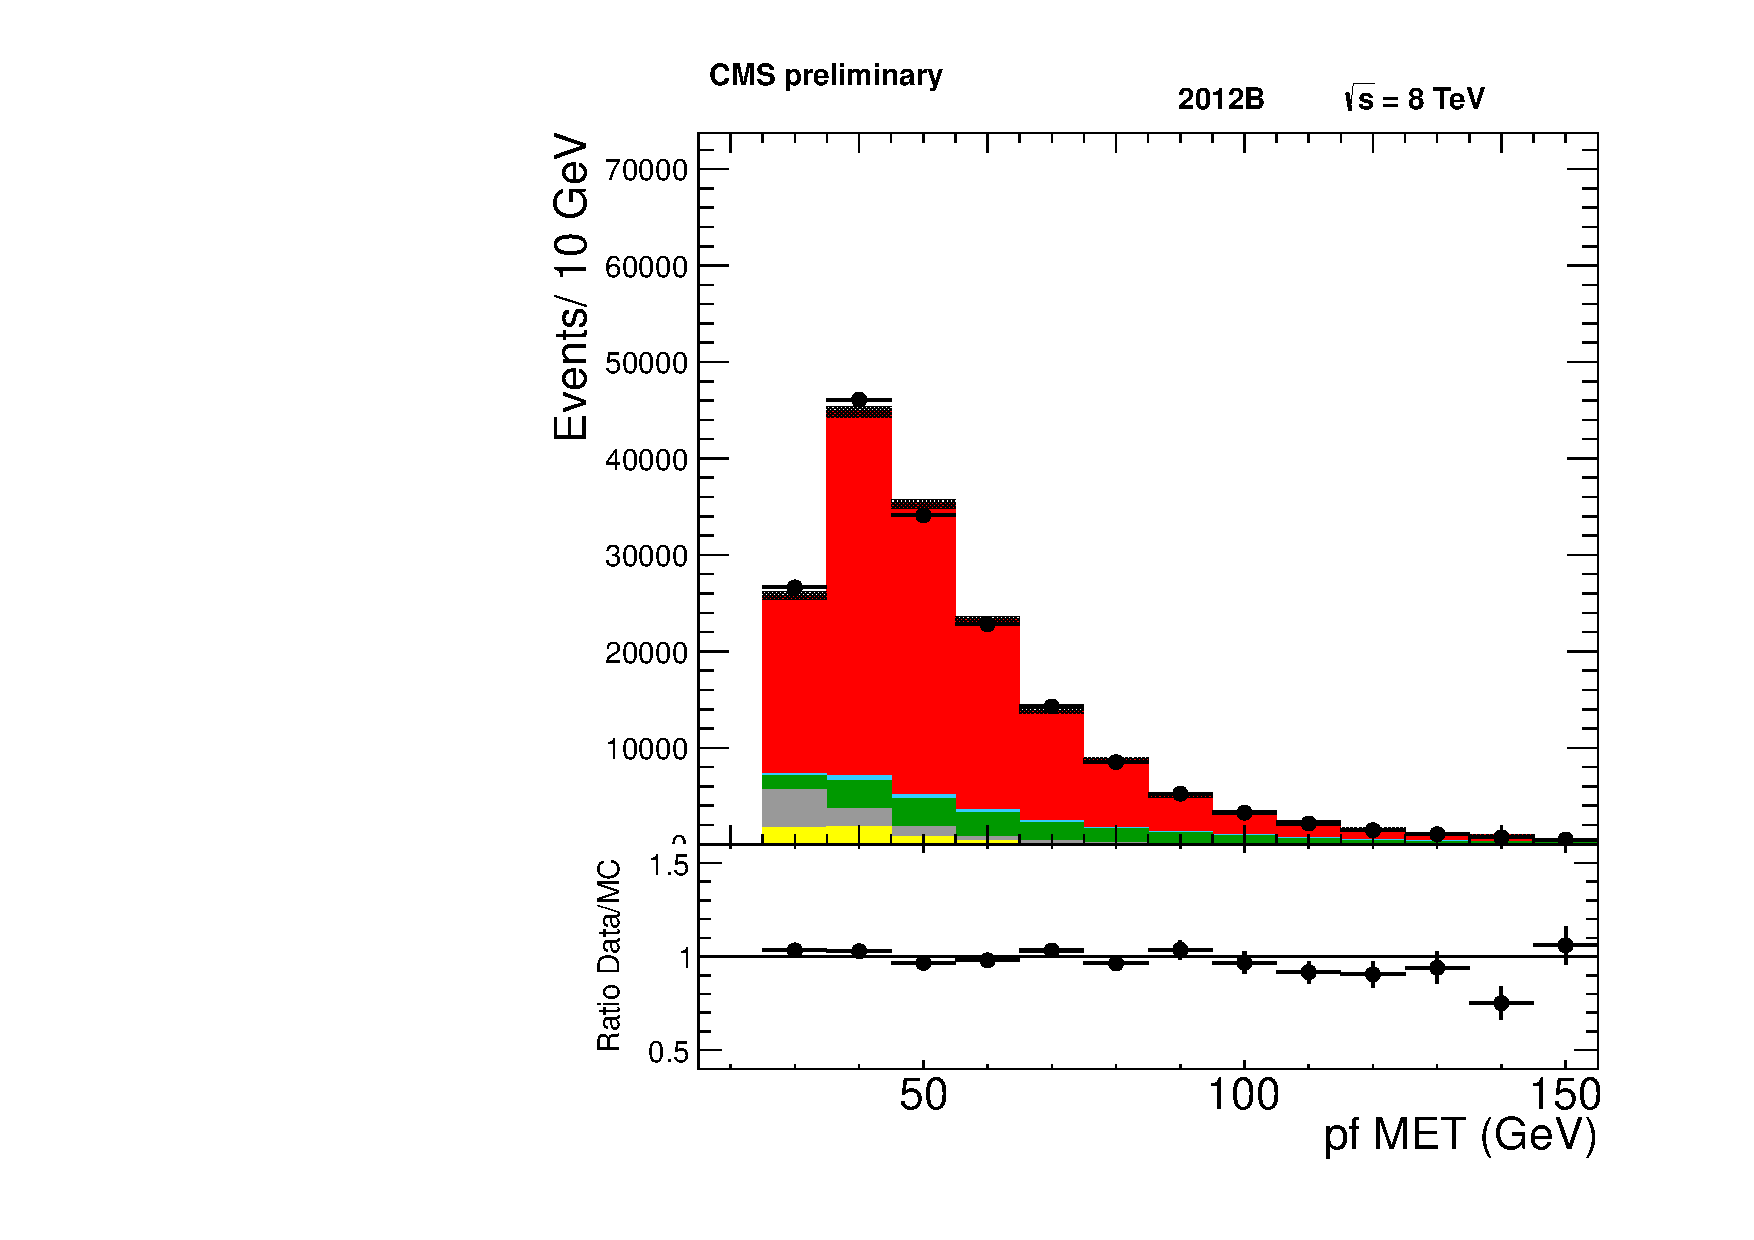
\includegraphics[width=0.4\textwidth]{plots/el_event_met_pfmet_2012B.pdf}
    }
    \\
    \subfigure[2012A: dijet mass($m_{jj}$)]{
      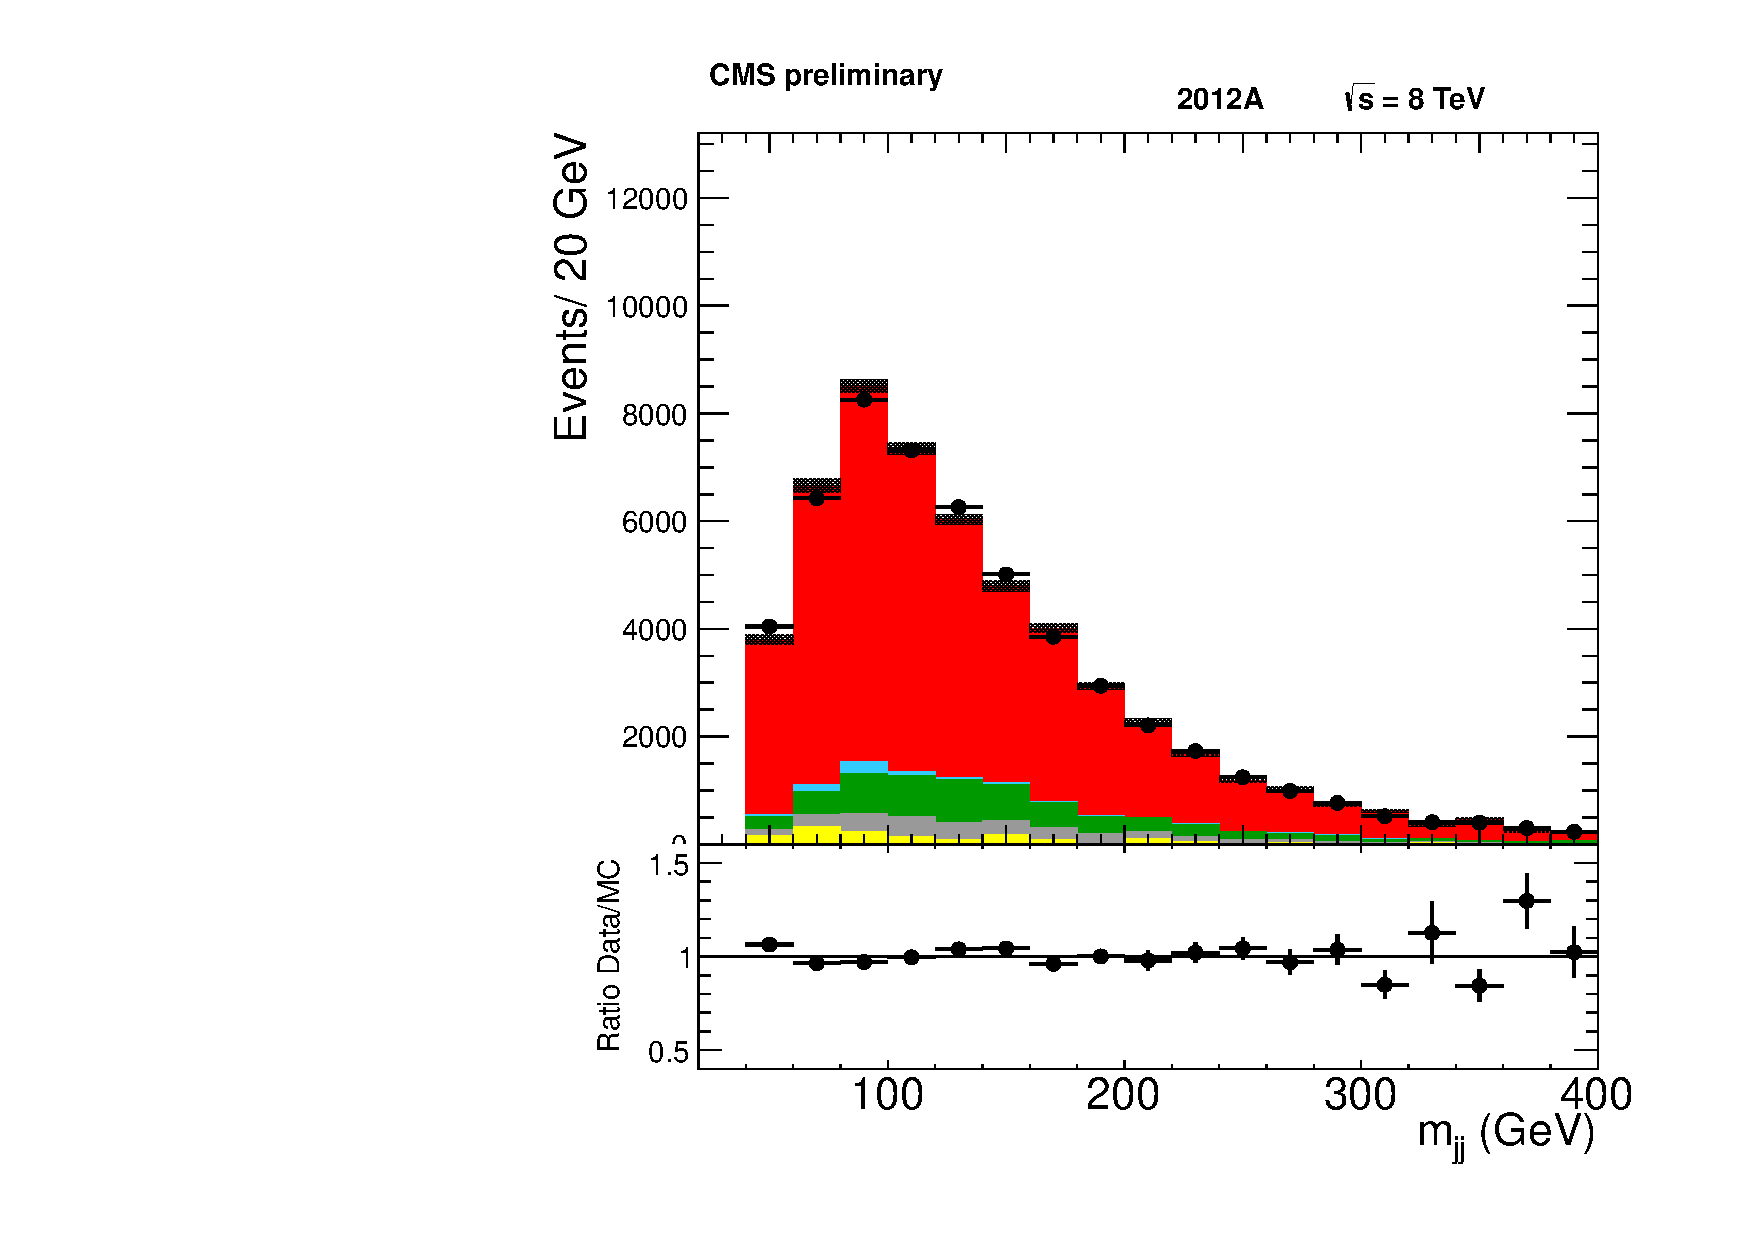
\includegraphics[width=0.4\textwidth]{plots/el_mjj_2012A.pdf}
    }
    \subfigure[2012B: dijet mass($m_{jj}$)]{
      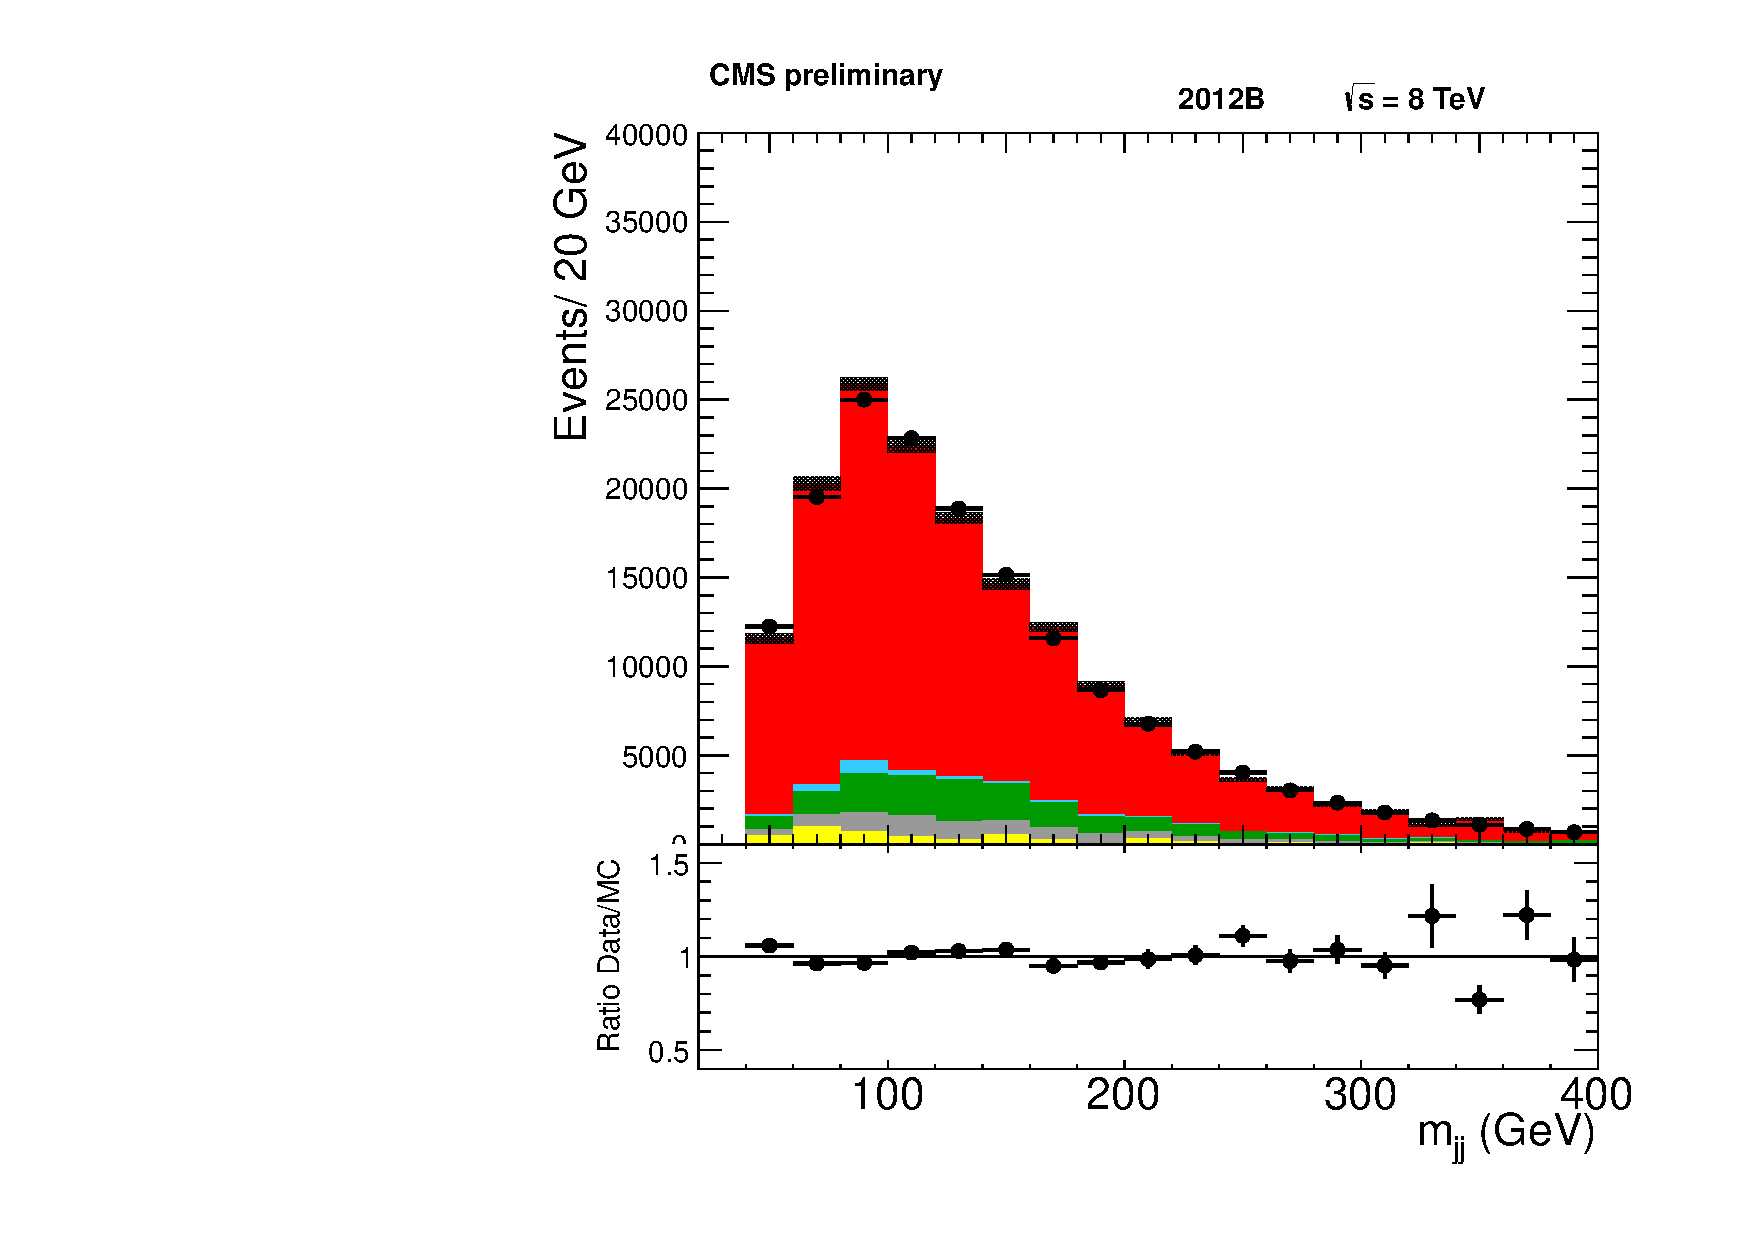
\includegraphics[width=0.4\textwidth]{plots/el_mjj_2012B.pdf}
    }
    \\
    \caption{
             Comparison of the MET and the dijet mass($m_{jj}$) distributions from data and MC for the 
electron+jets selection.
            }
    \label{fig:CP2012AB6}
\end{figure}


\begin{figure}[htb]
  \centering
    \subfigure[2012A: $\cos\theta_{1}$]{
      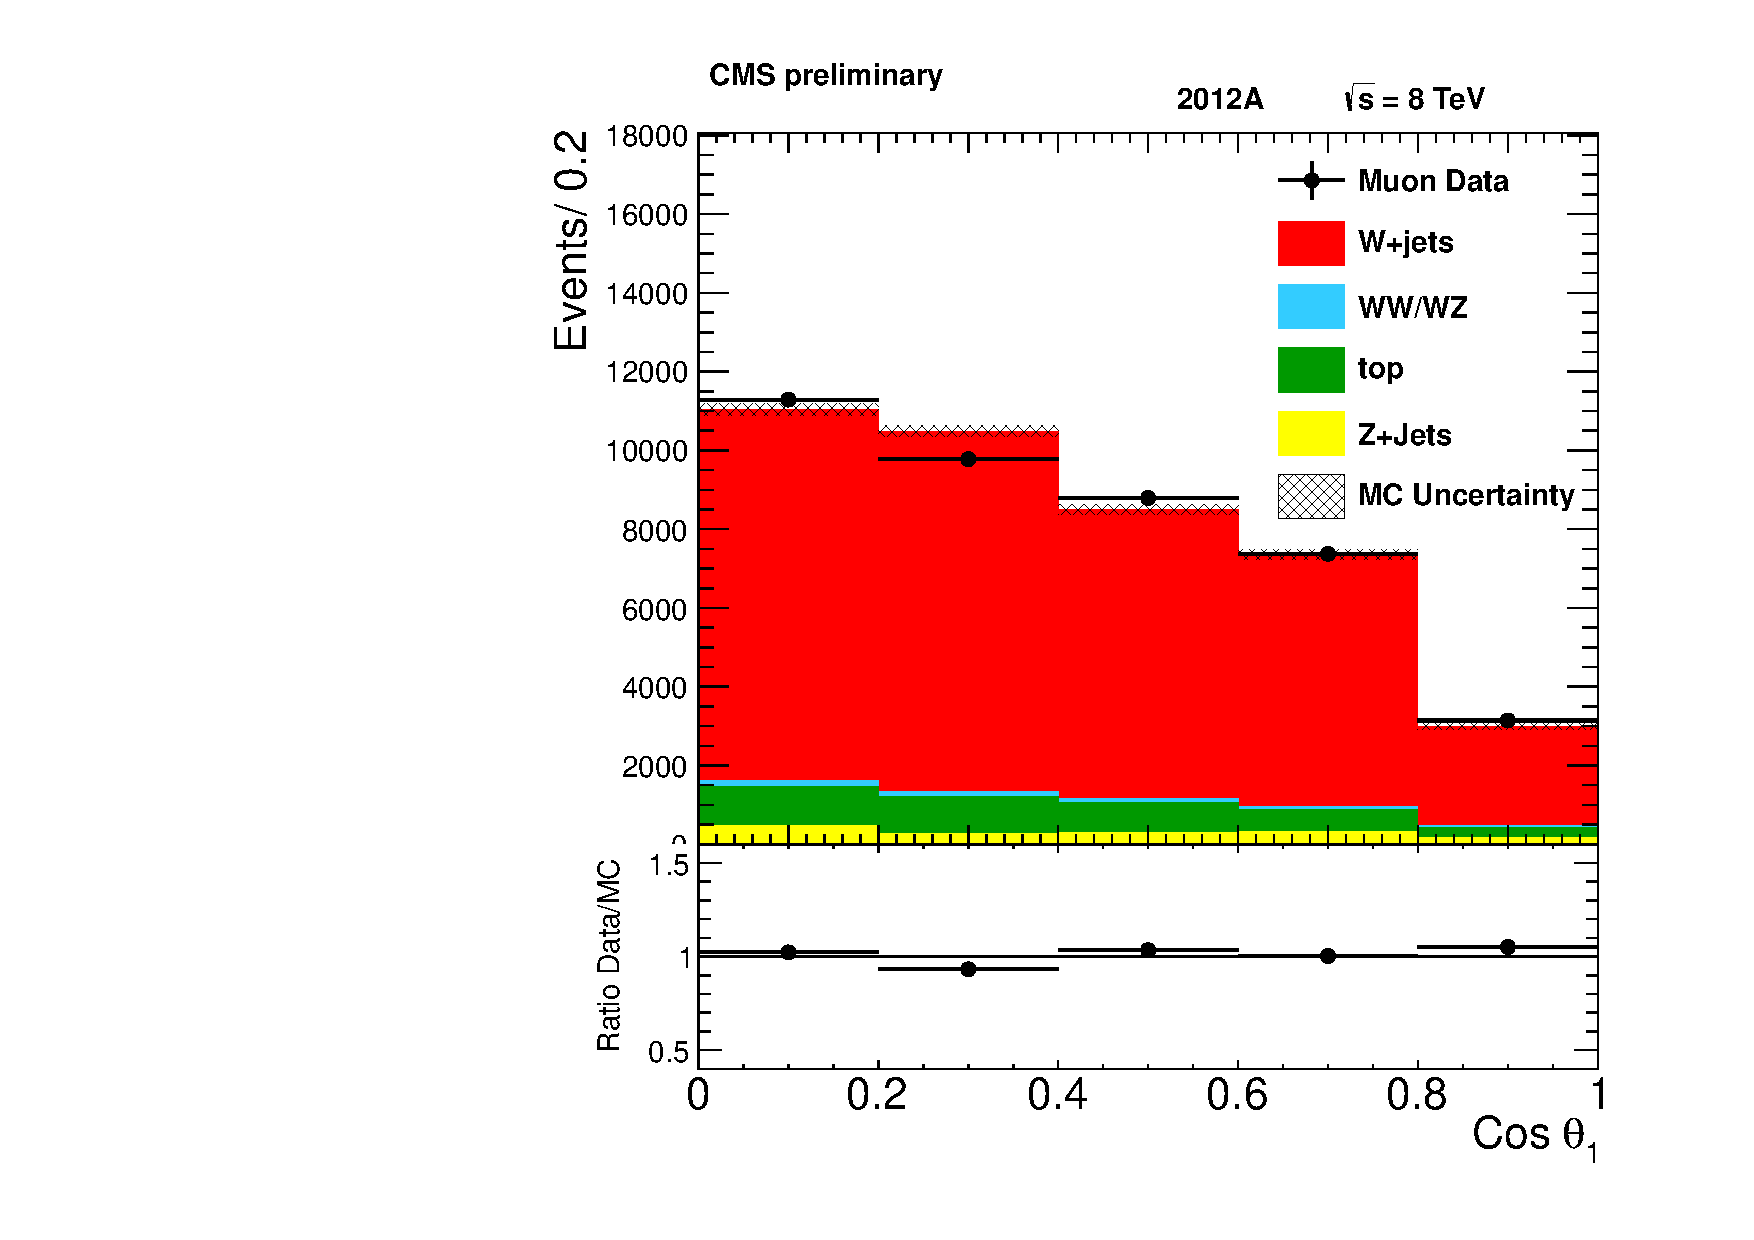
\includegraphics[width=0.4\textwidth]{plots/mu_ha_2012A.pdf}
    }
    \subfigure[2012B: $\cos\theta_{1}$]{
      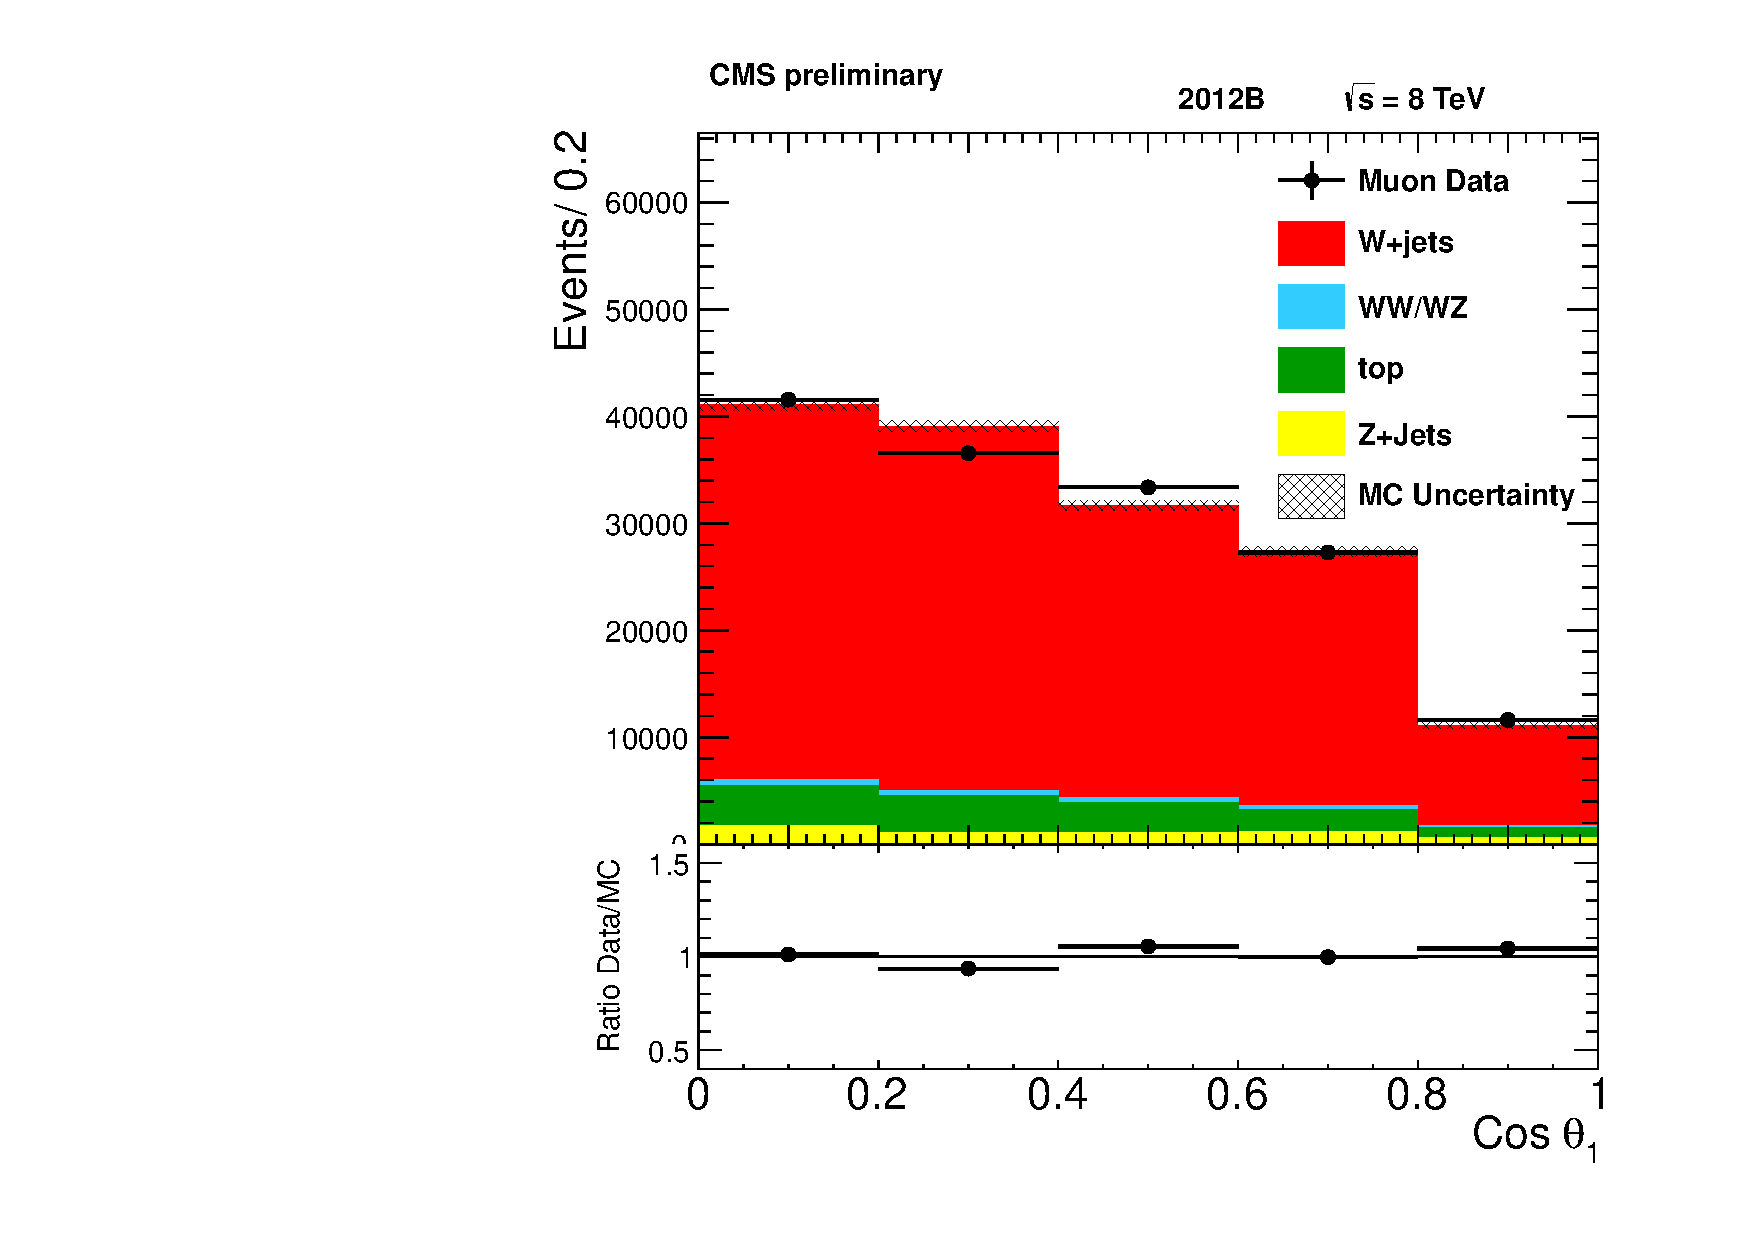
\includegraphics[width=0.4\textwidth]{plots/mu_ha_2012B.pdf}
    }
    \\
    \subfigure[2012A: $\cos\theta_{2}$]{
      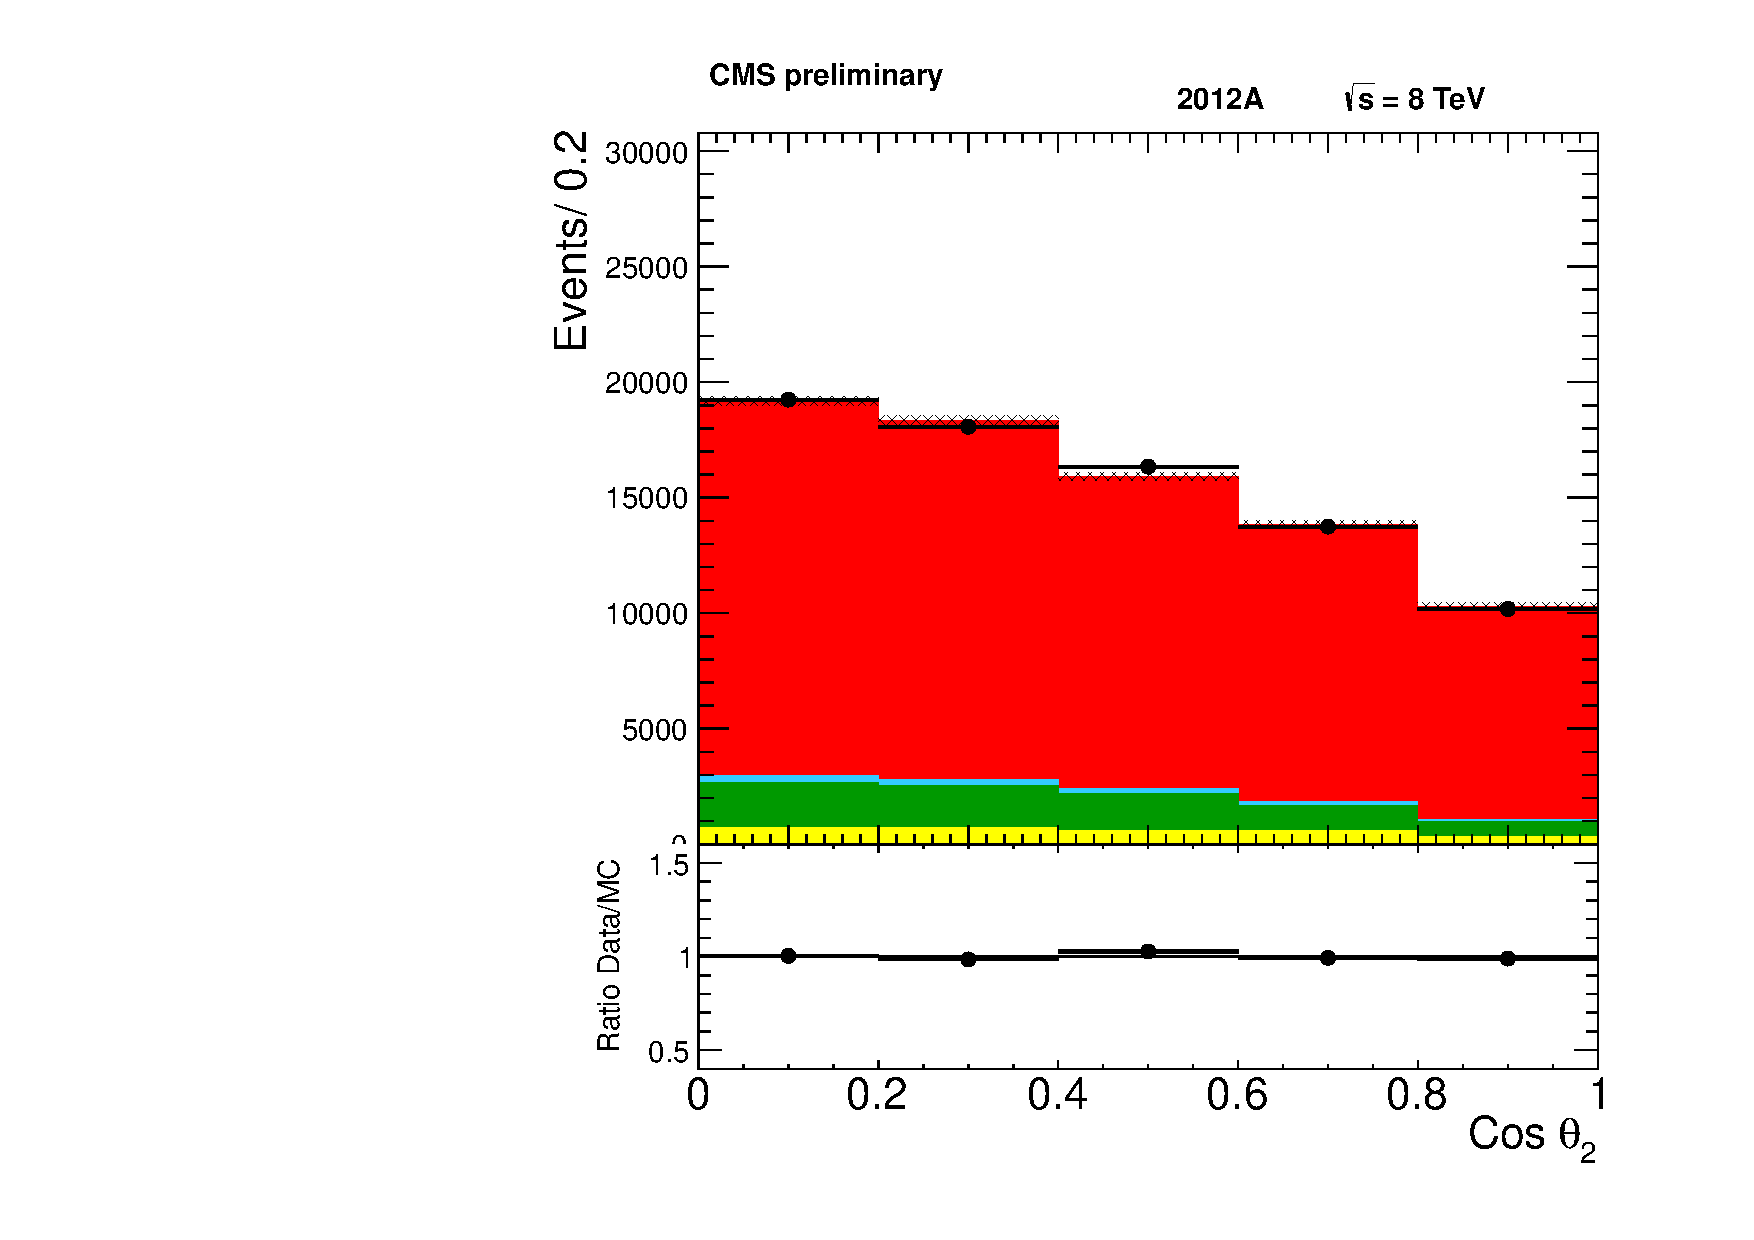
\includegraphics[width=0.4\textwidth]{plots/mu_hb_2012A.pdf}
    }
    \subfigure[2012B: $\cos\theta_{2}$]{
      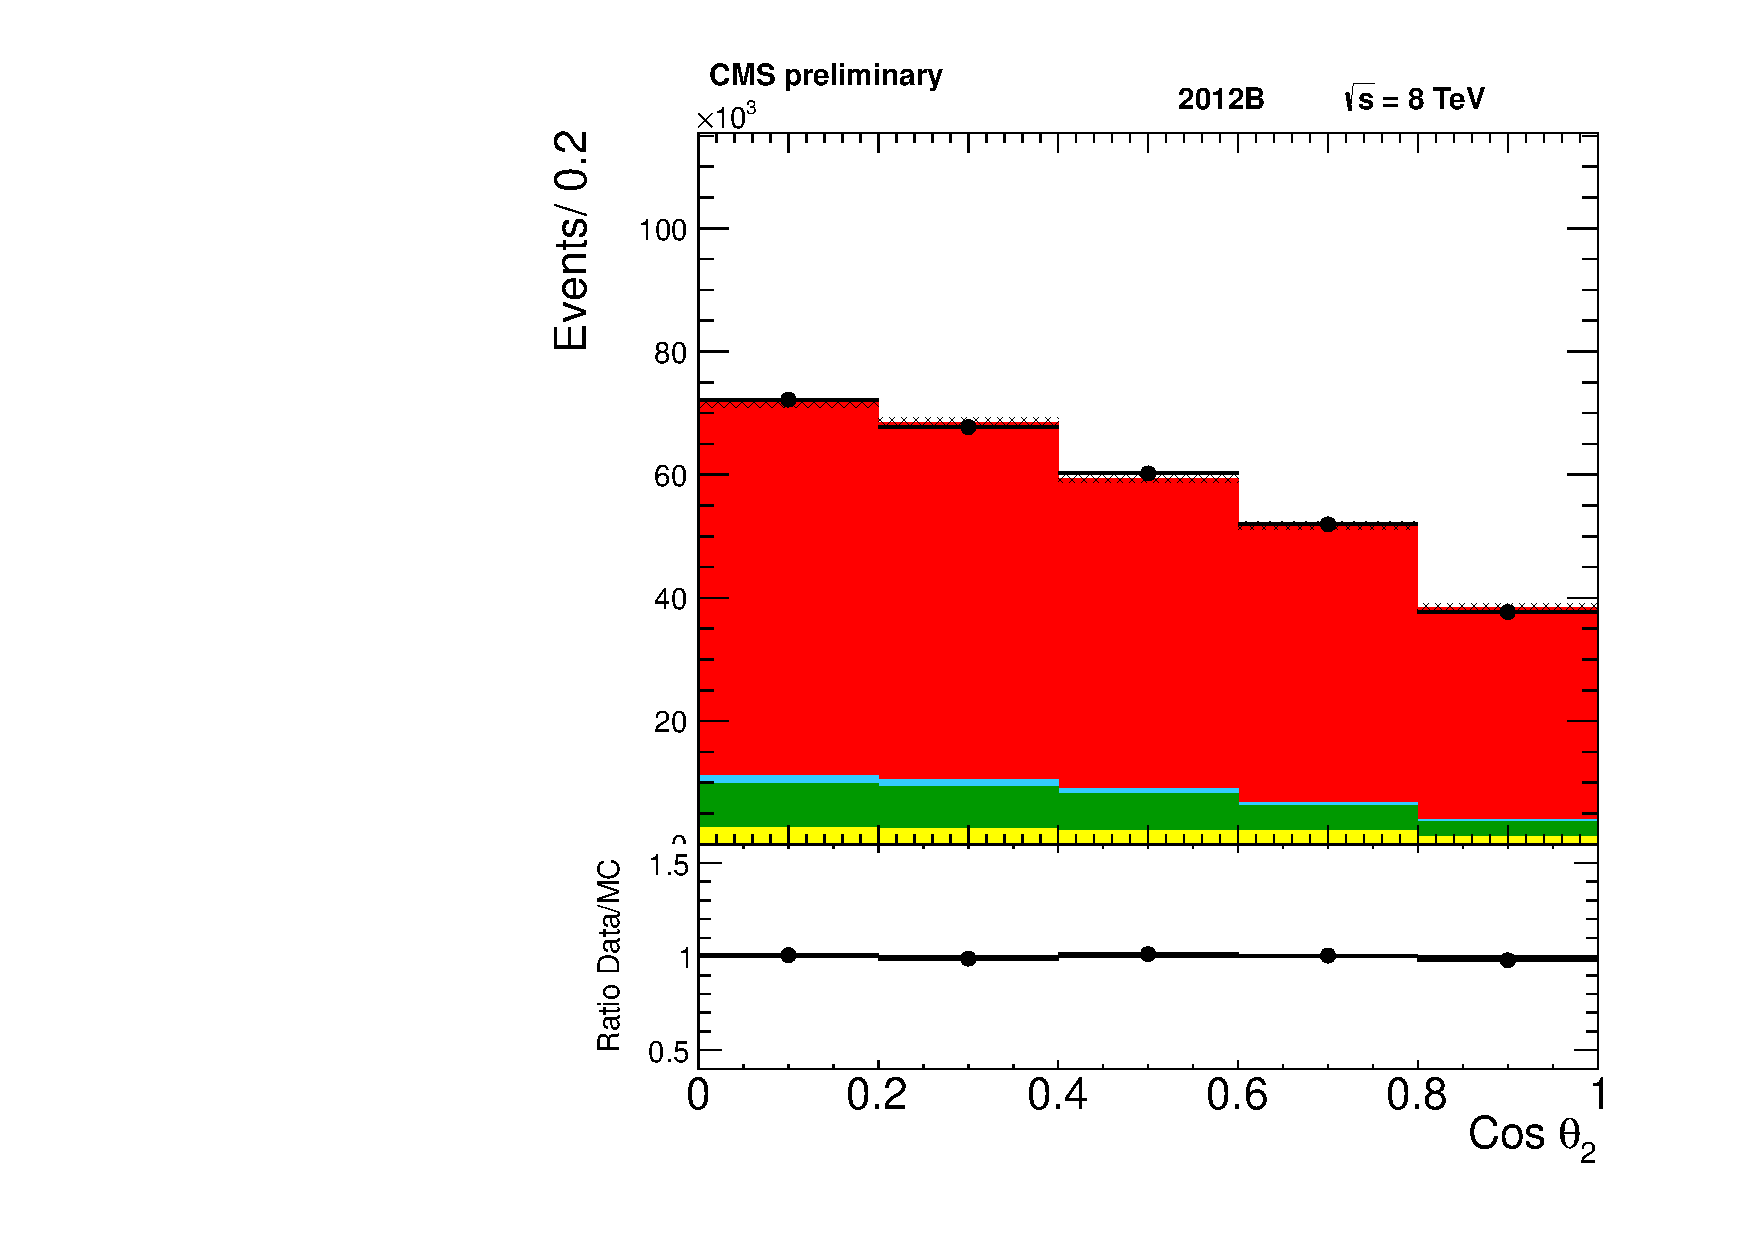
\includegraphics[width=0.4\textwidth]{plots/mu_hb_2012B.pdf}
    }
    \\
    \subfigure[2012A: $\cos\theta^{\ast}$]{
      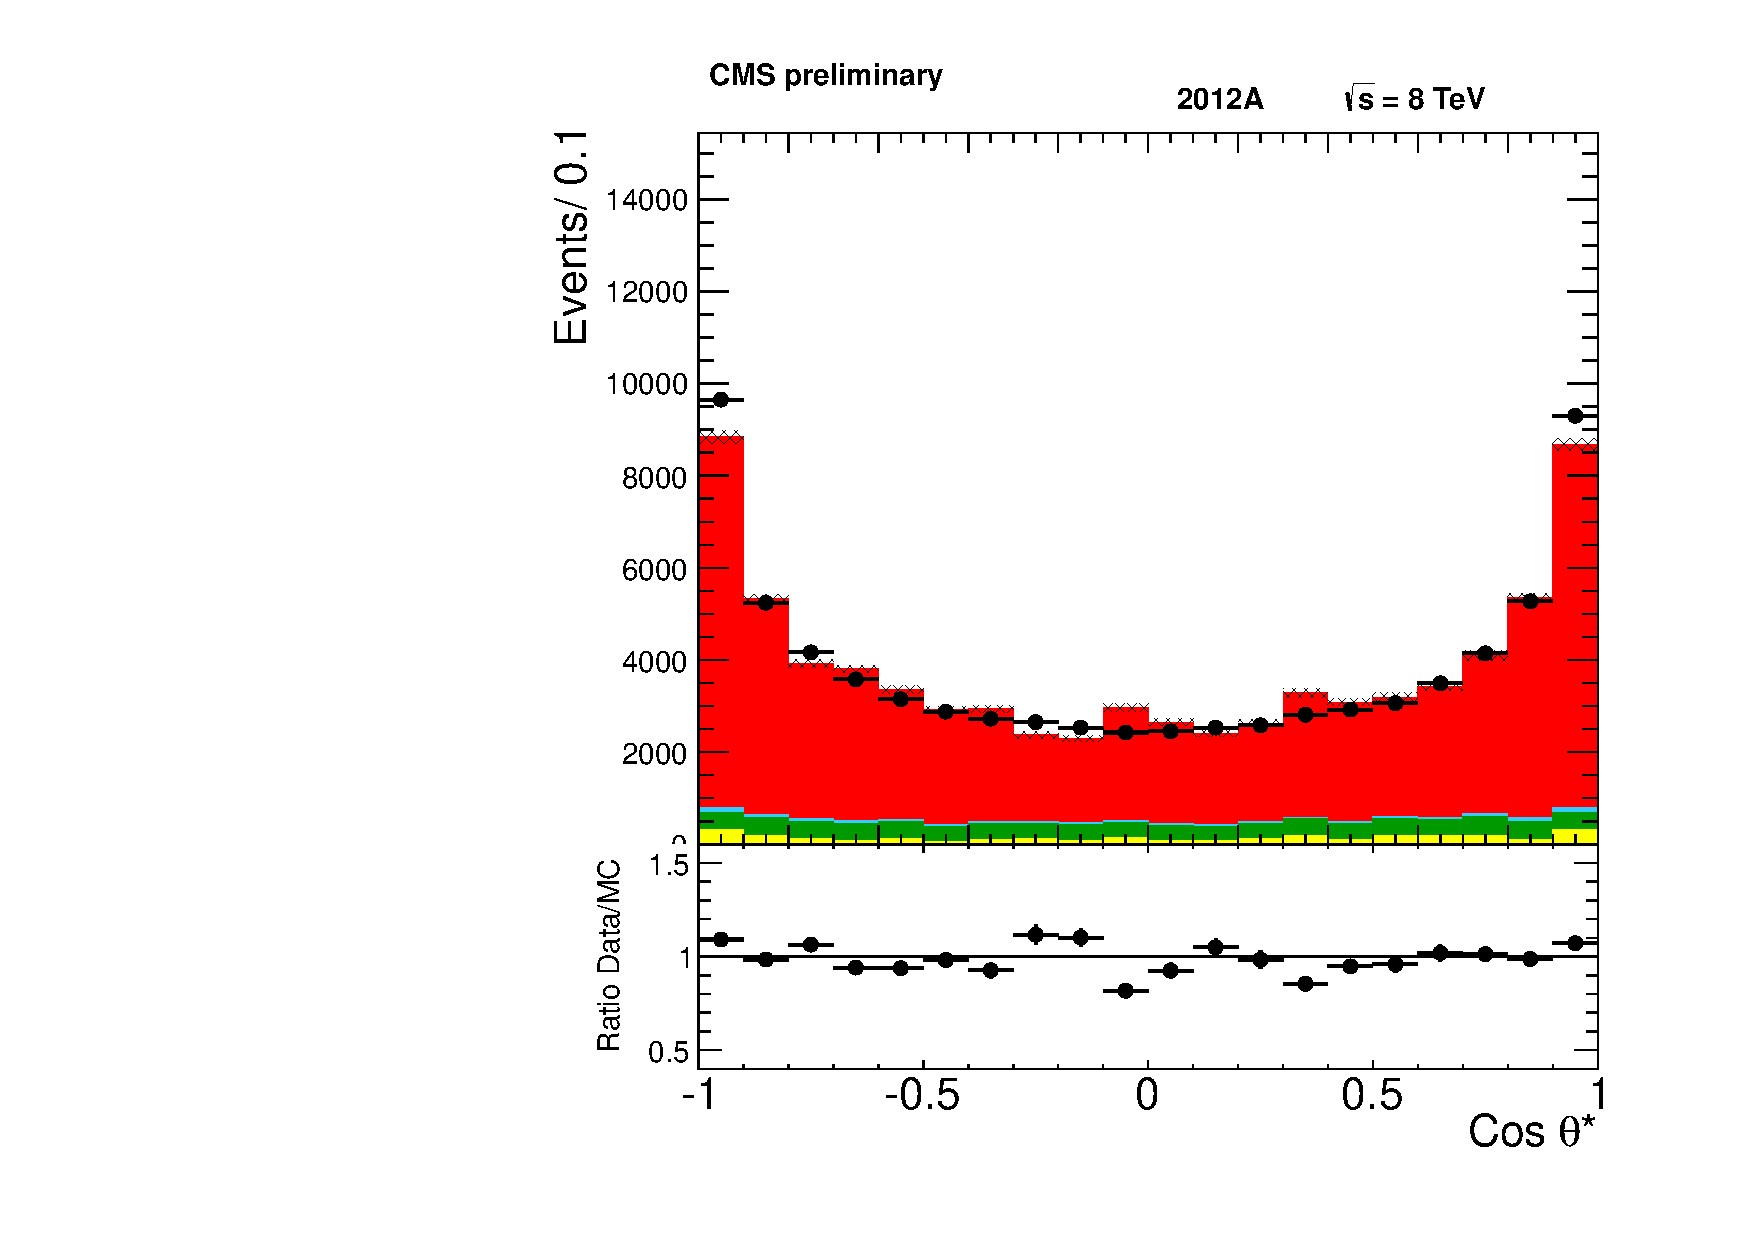
\includegraphics[width=0.4\textwidth]{plots/mu_hs_2012A.pdf}
    }
    \subfigure[2012B: $\cos\theta^{\ast}$]{
      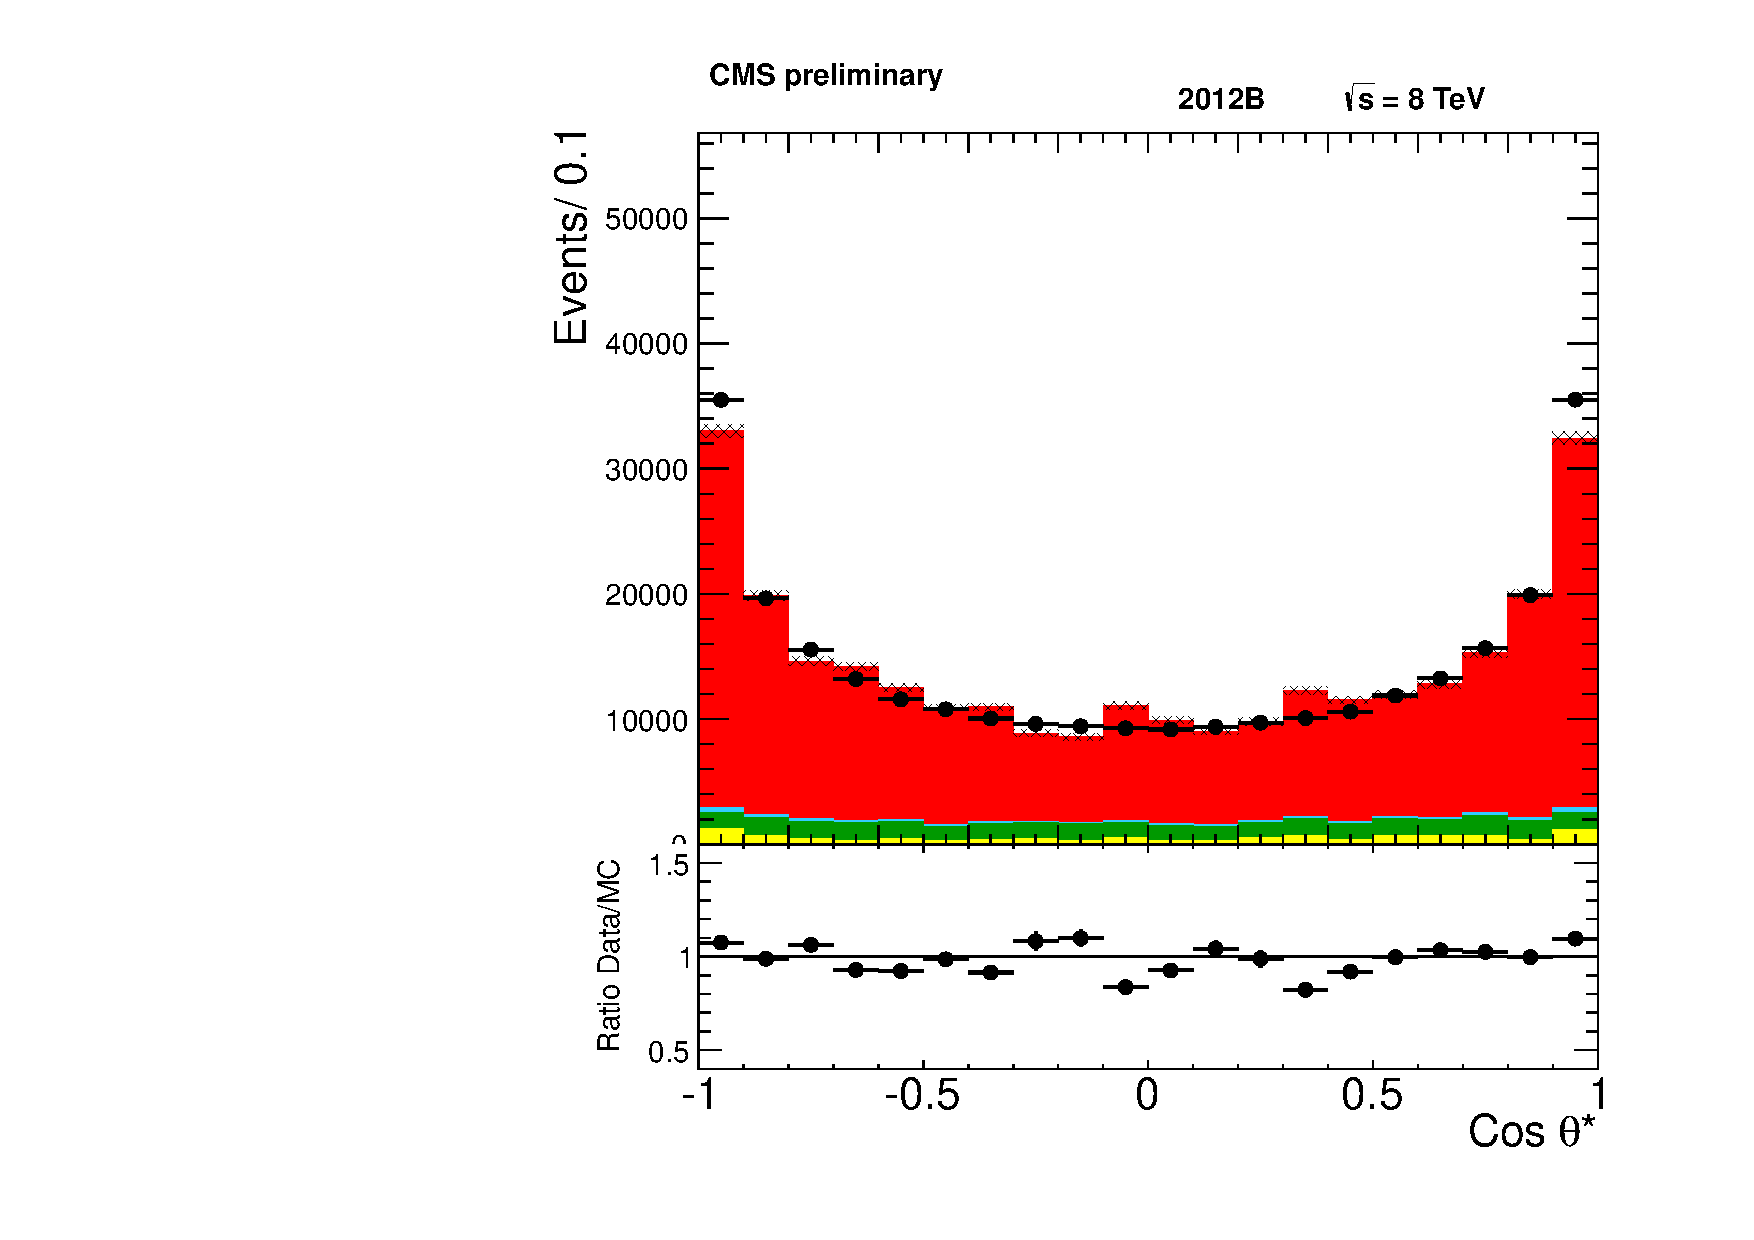
\includegraphics[width=0.4\textwidth]{plots/mu_hs_2012B.pdf}
    }
    \\
    \caption{ Comparison of the angular distributions for $\cos\theta_{1}$,$\cos\theta_{2}$ and $\cos\theta^{\ast}$ from data and MC for 
the muon+jets selection.
            }
    \label{fig:CP2012AB7}
\end{figure}




\begin{figure}[htb]
  \centering
    \subfigure[2012A: $\Phi$]{
      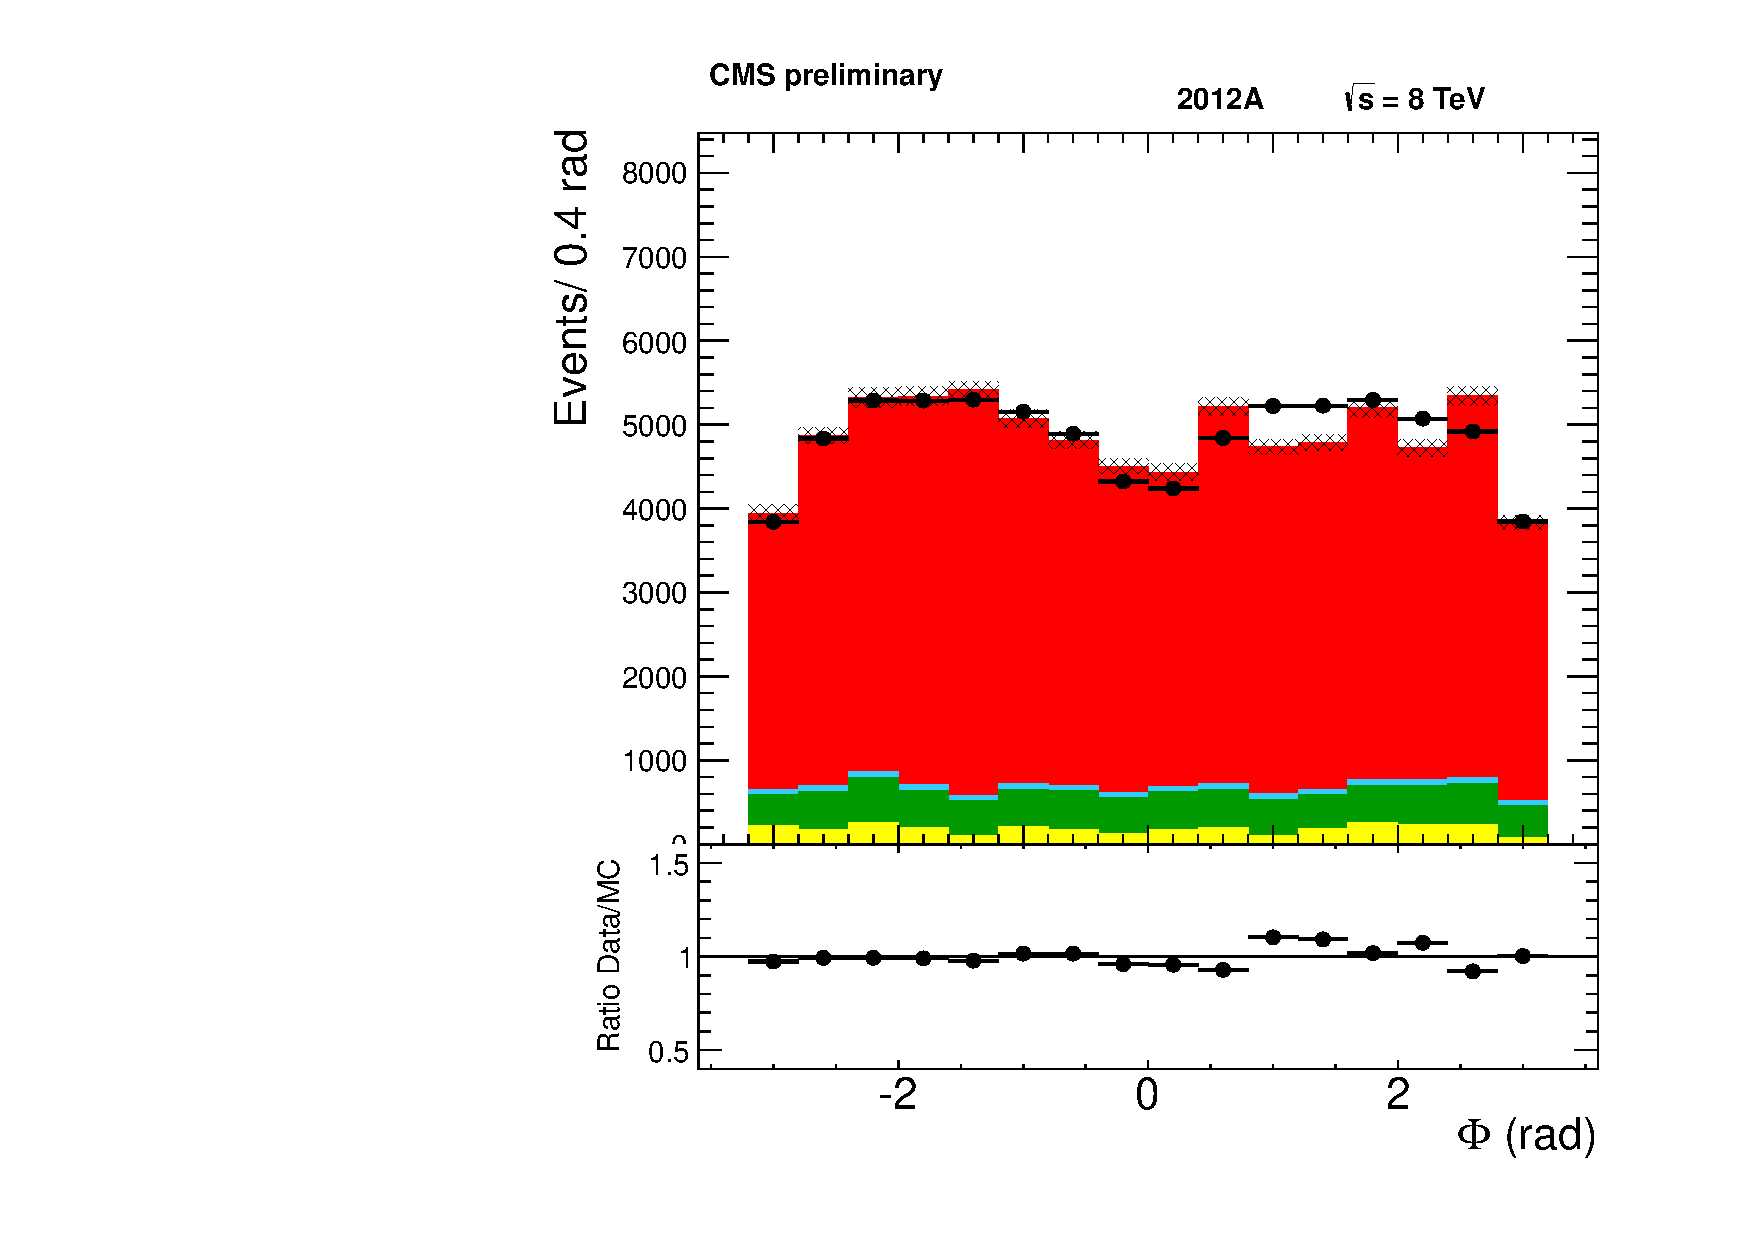
\includegraphics[width=0.4\textwidth]{plots/mu_phi_2012A.pdf}
    }
    \subfigure[2012B: $\Phi$]{
      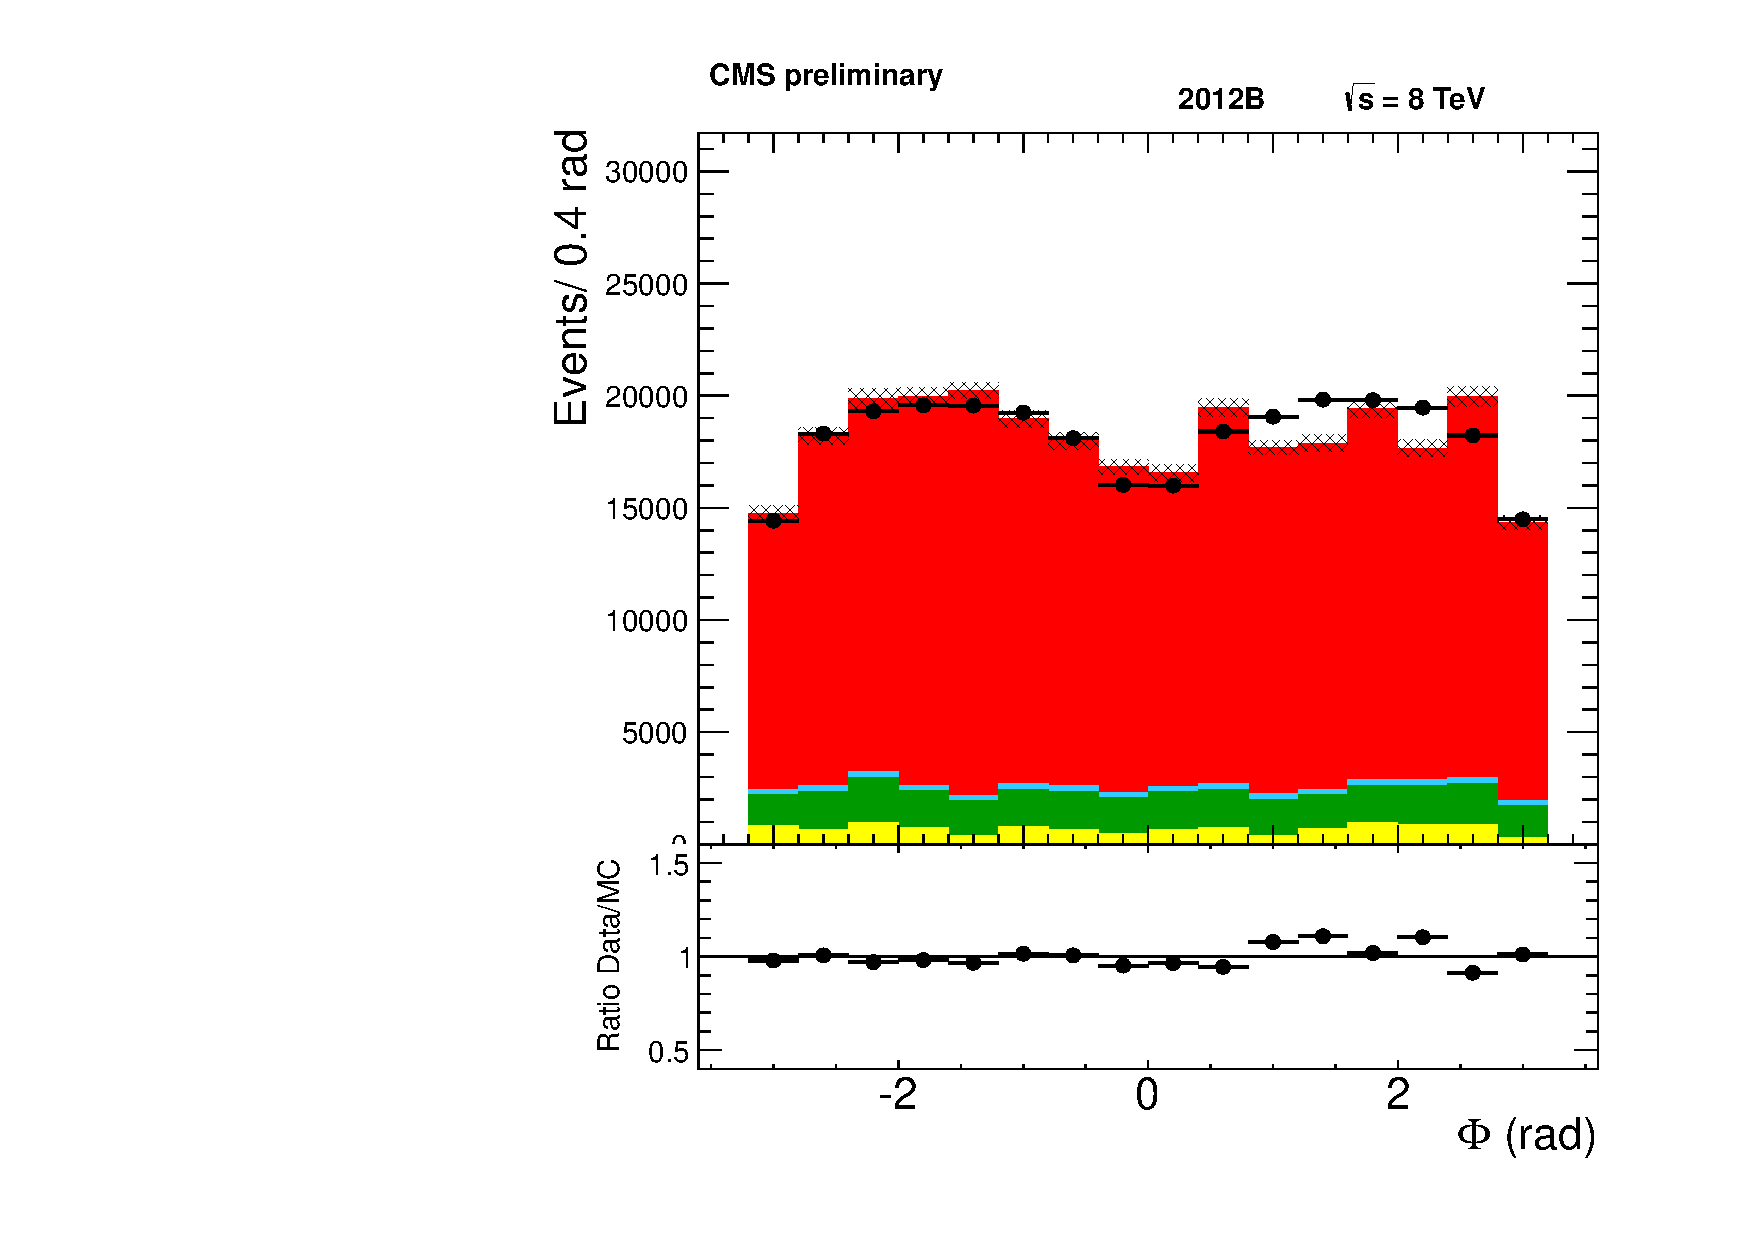
\includegraphics[width=0.4\textwidth]{plots/mu_phi_2012B.pdf}
    }
    \\
    \subfigure[2012A: $\Phi_{1}$]{
      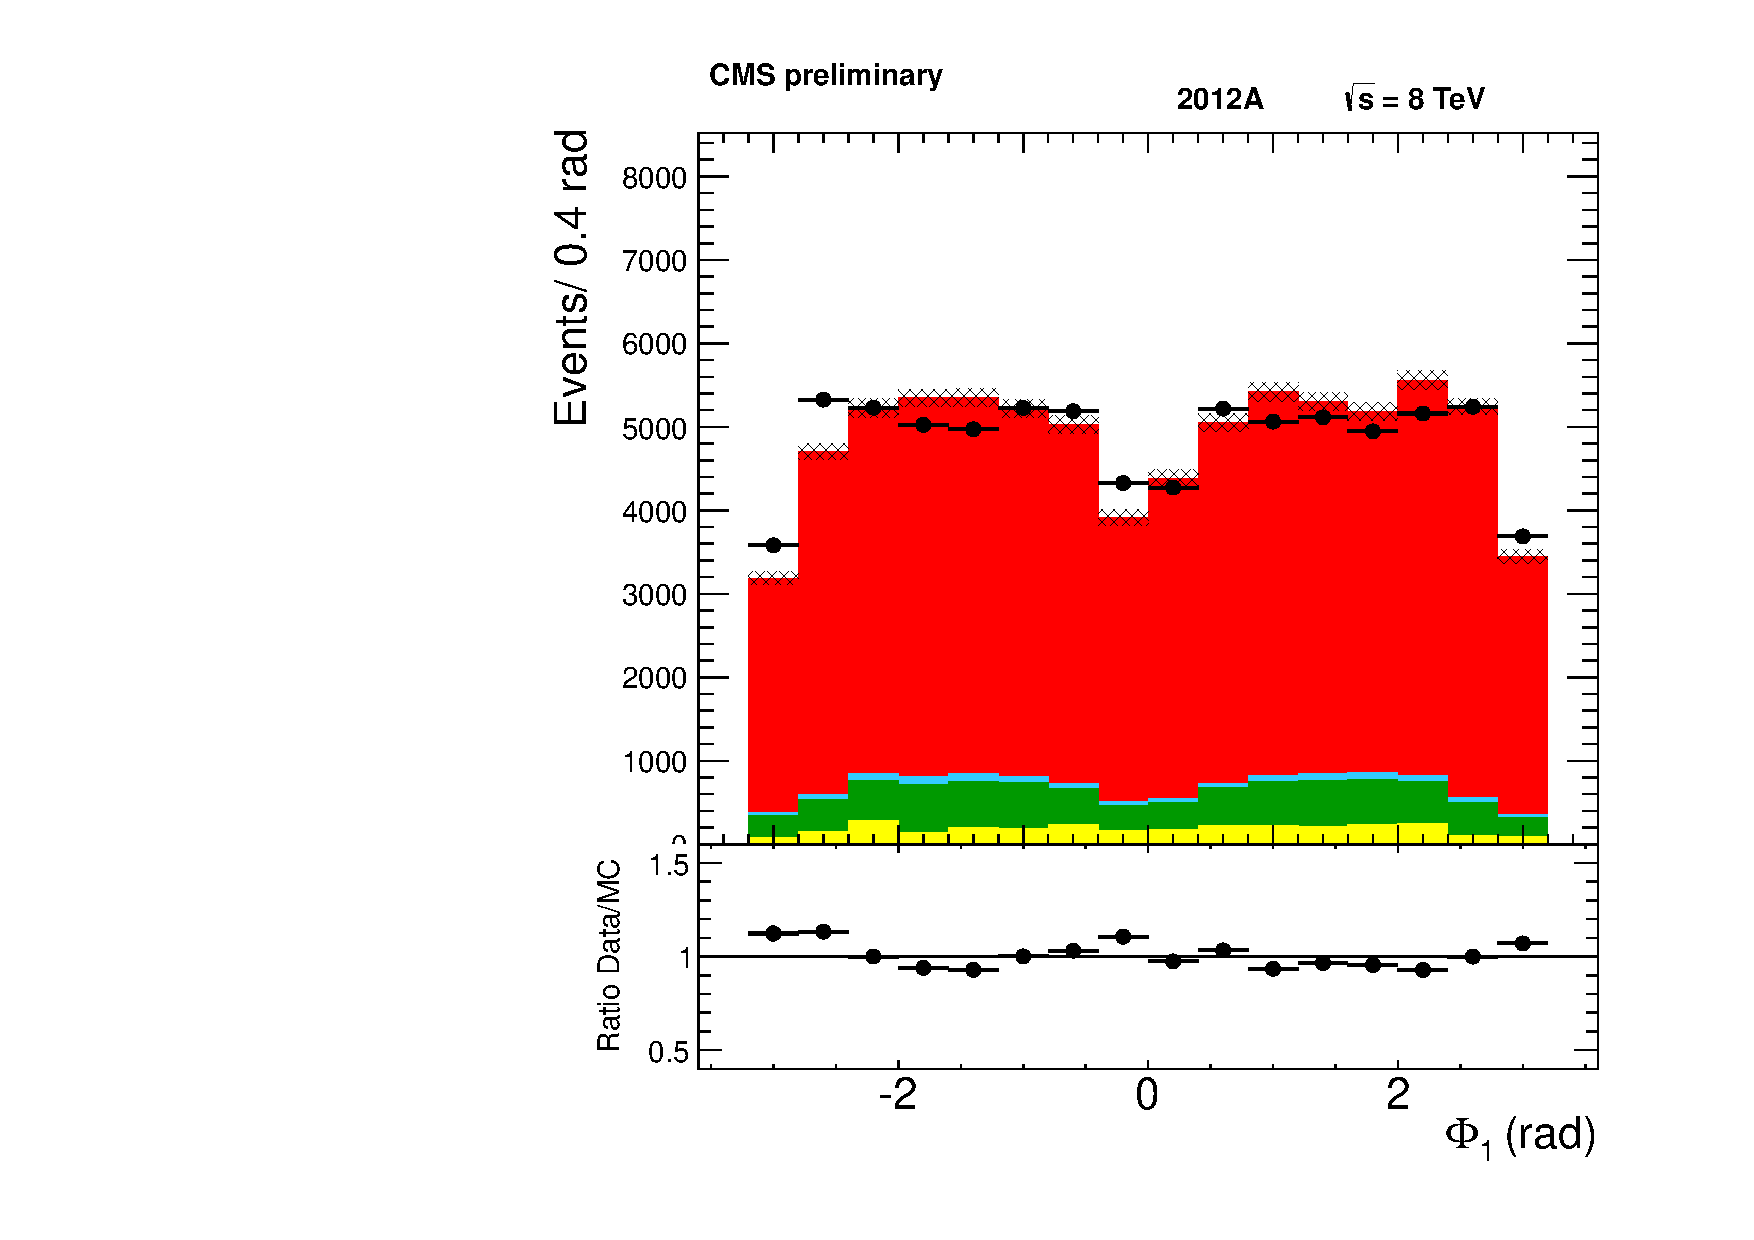
\includegraphics[width=0.4\textwidth]{plots/mu_phib_2012A.pdf}
    }
    \subfigure[2012B: $\Phi_{1}$]{
      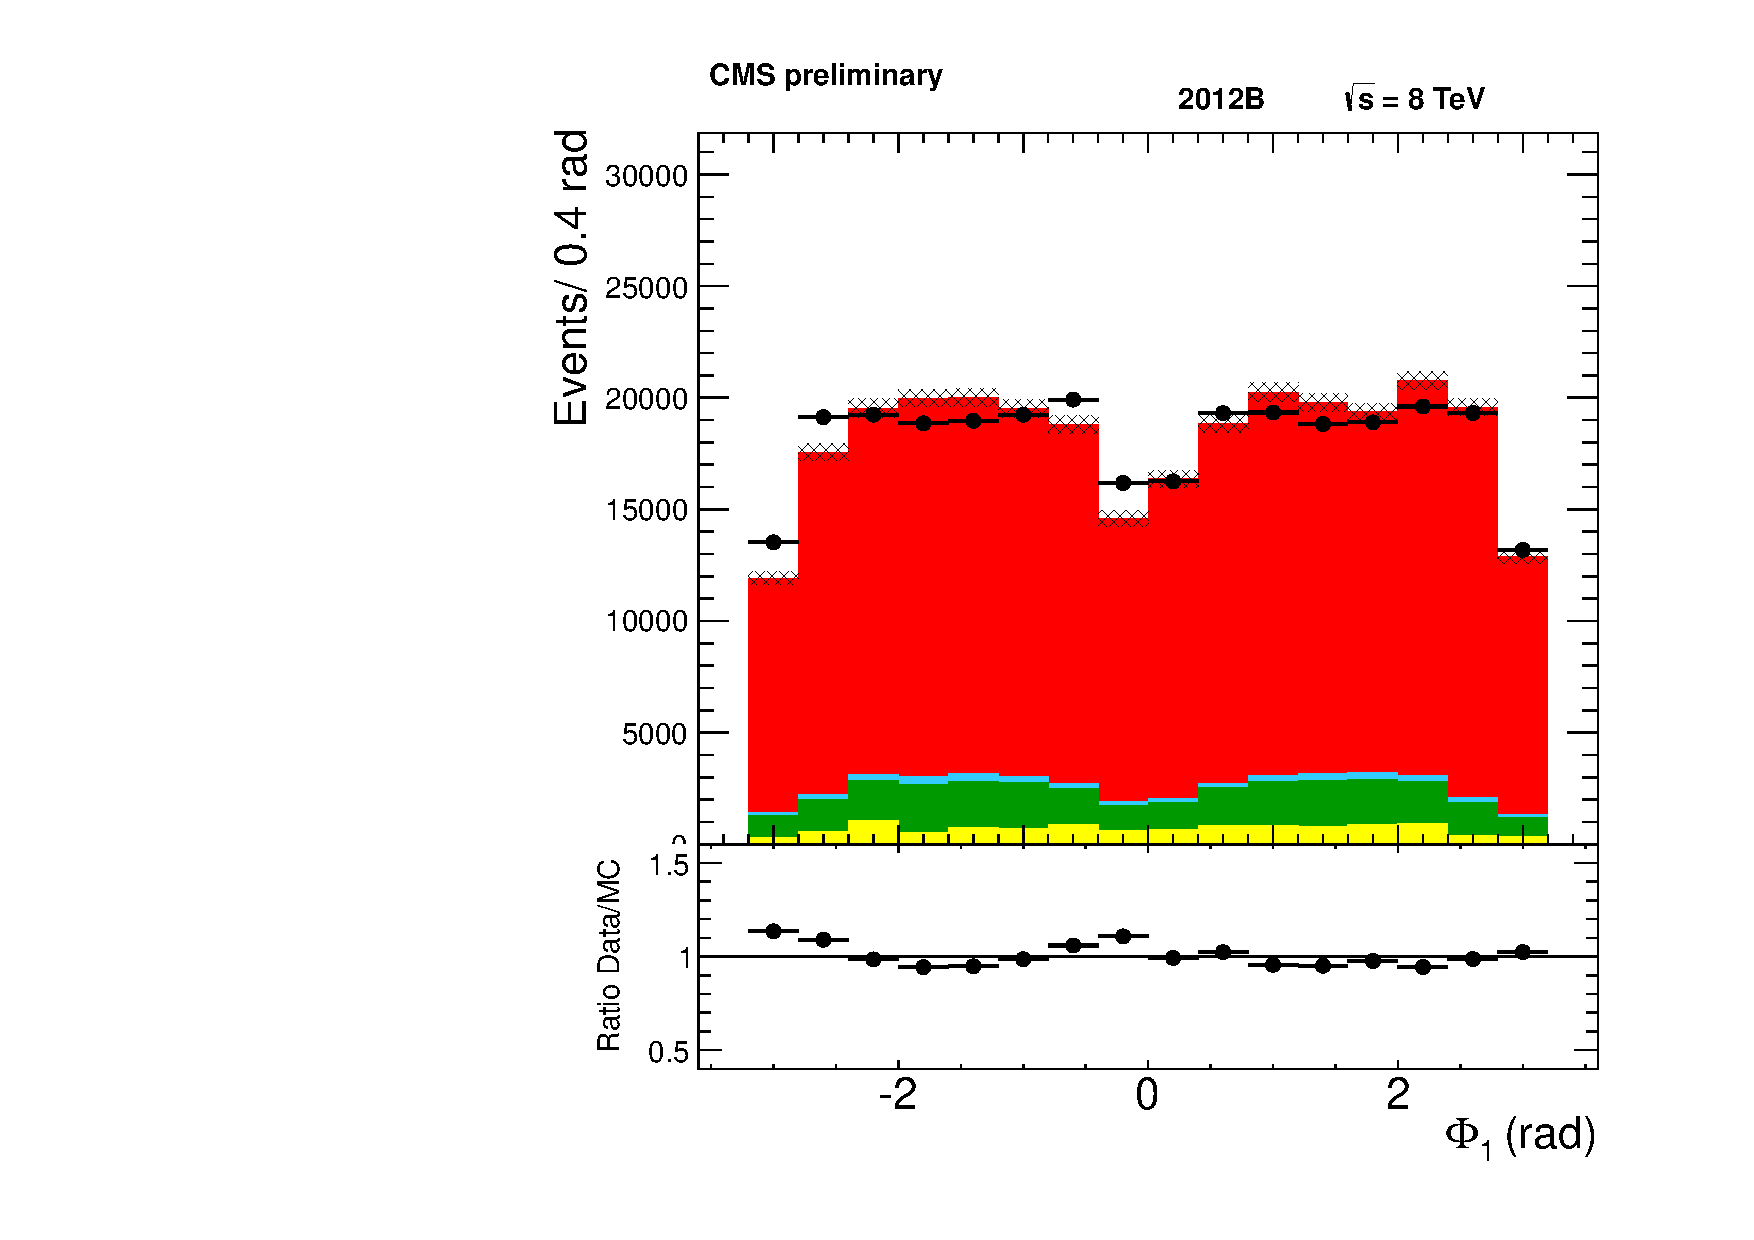
\includegraphics[width=0.4\textwidth]{plots/mu_phib_2012B.pdf}
    }
    \\
    \subfigure[2012A: muon charge]{
      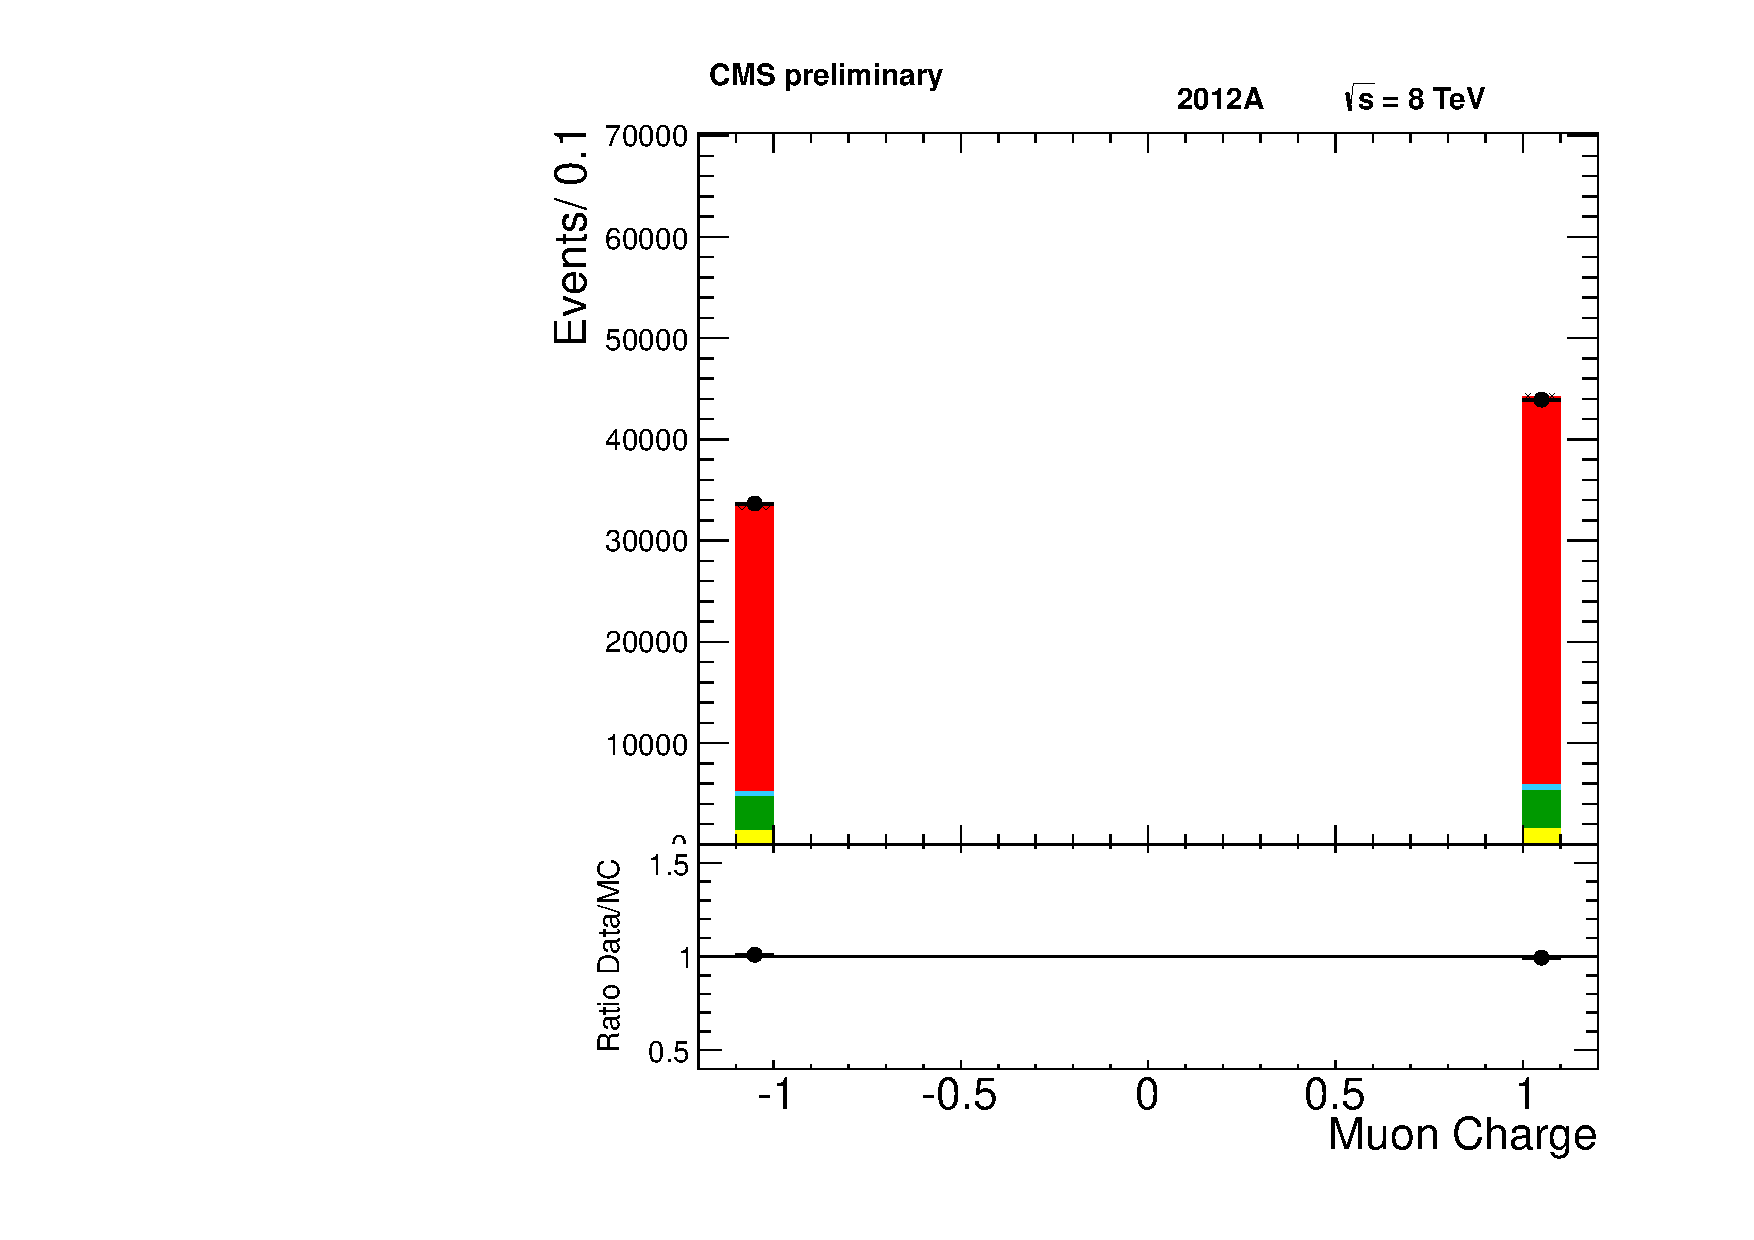
\includegraphics[width=0.4\textwidth]{plots/mu_charge_2012A.pdf}
    }
    \subfigure[2012B: muon charge]{
      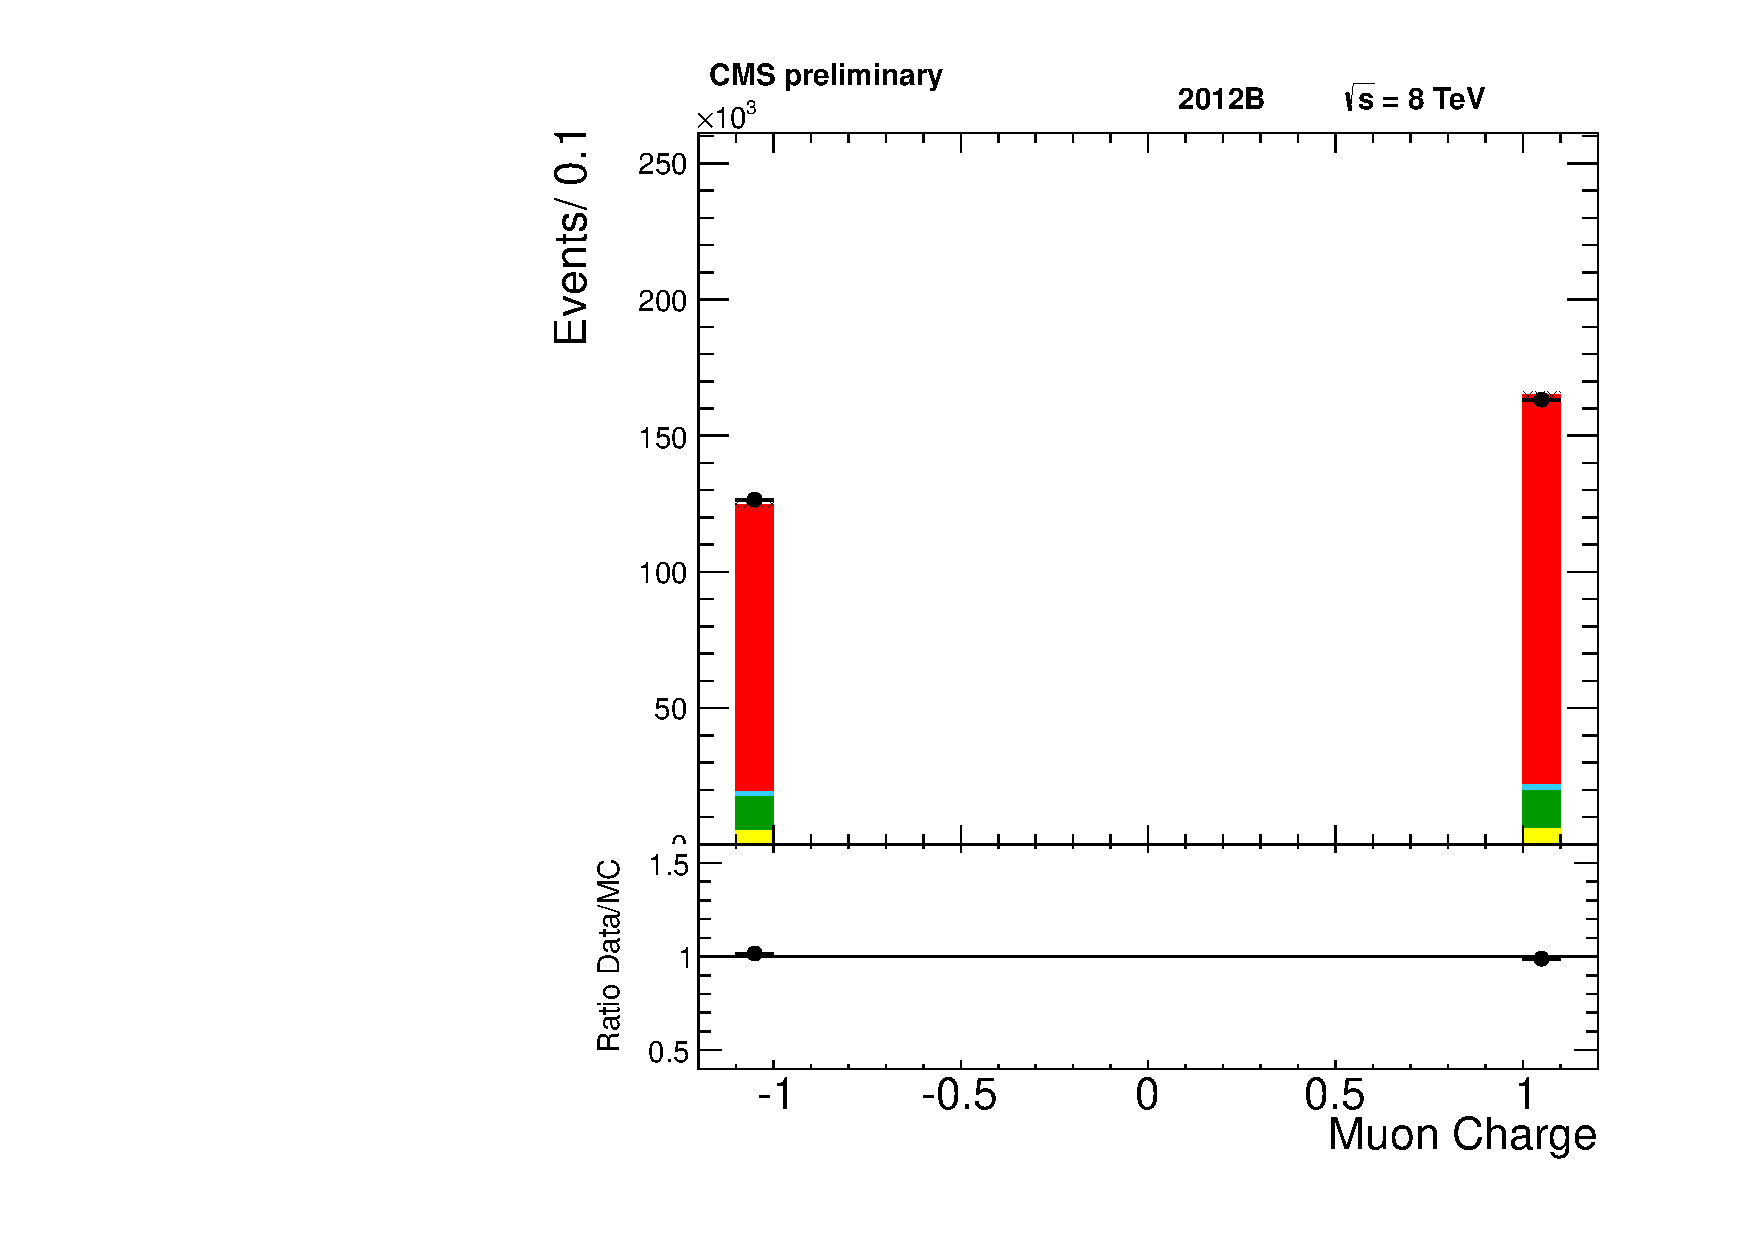
\includegraphics[width=0.4\textwidth]{plots/mu_charge_2012B.pdf}
    }
    \\
    \caption{ Comparison of the angular distributions for $\Phi$ , $\Phi_{1}$ and muon charge from data and MC for
the muon+jets selection.
            }
    \label{fig:CP2012AB8}
\end{figure}


\begin{figure}[htb]
  \centering
    \subfigure[2012A: WW $p_{T}$]{
      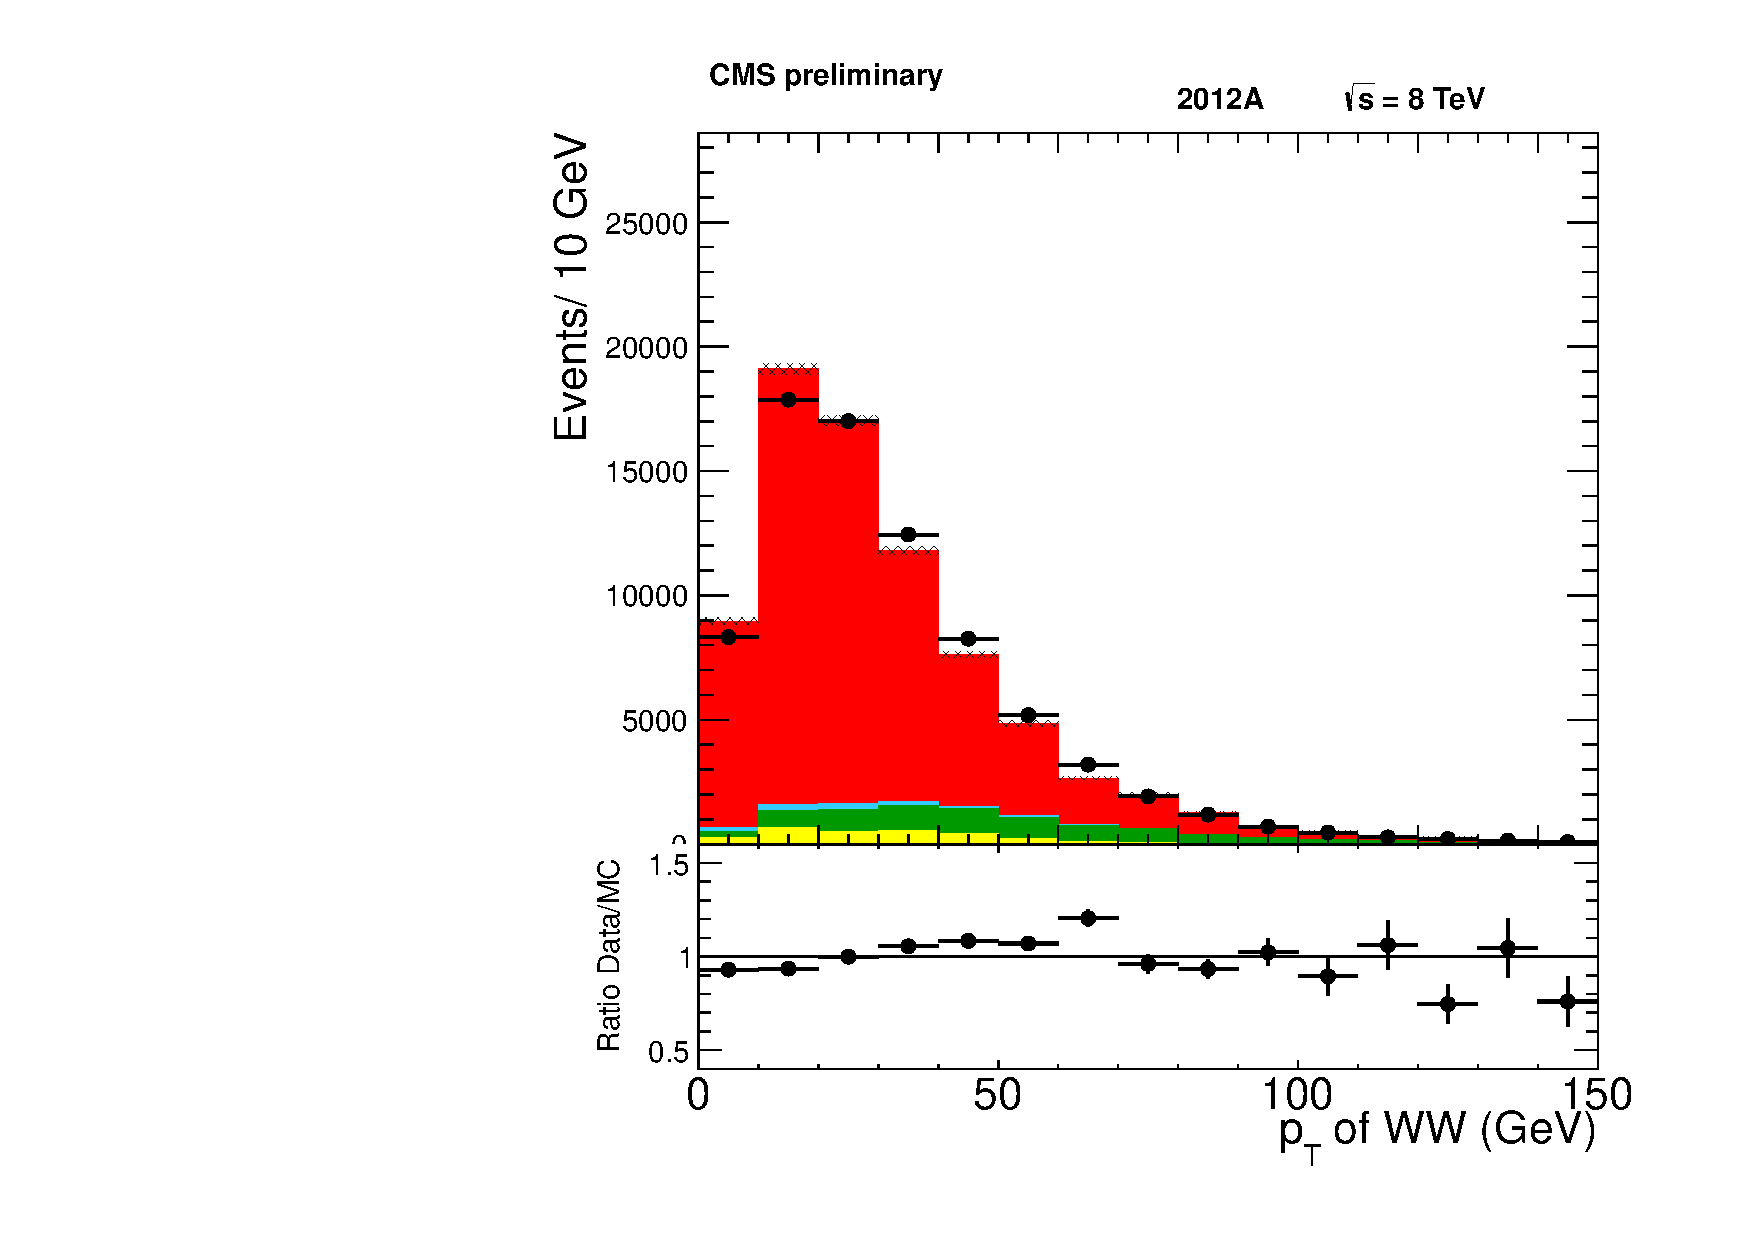
\includegraphics[width=0.4\textwidth]{plots/mu_ptlvjj_2012A.pdf}
    }
    \subfigure[2012B: WW $p_{T}$]{
      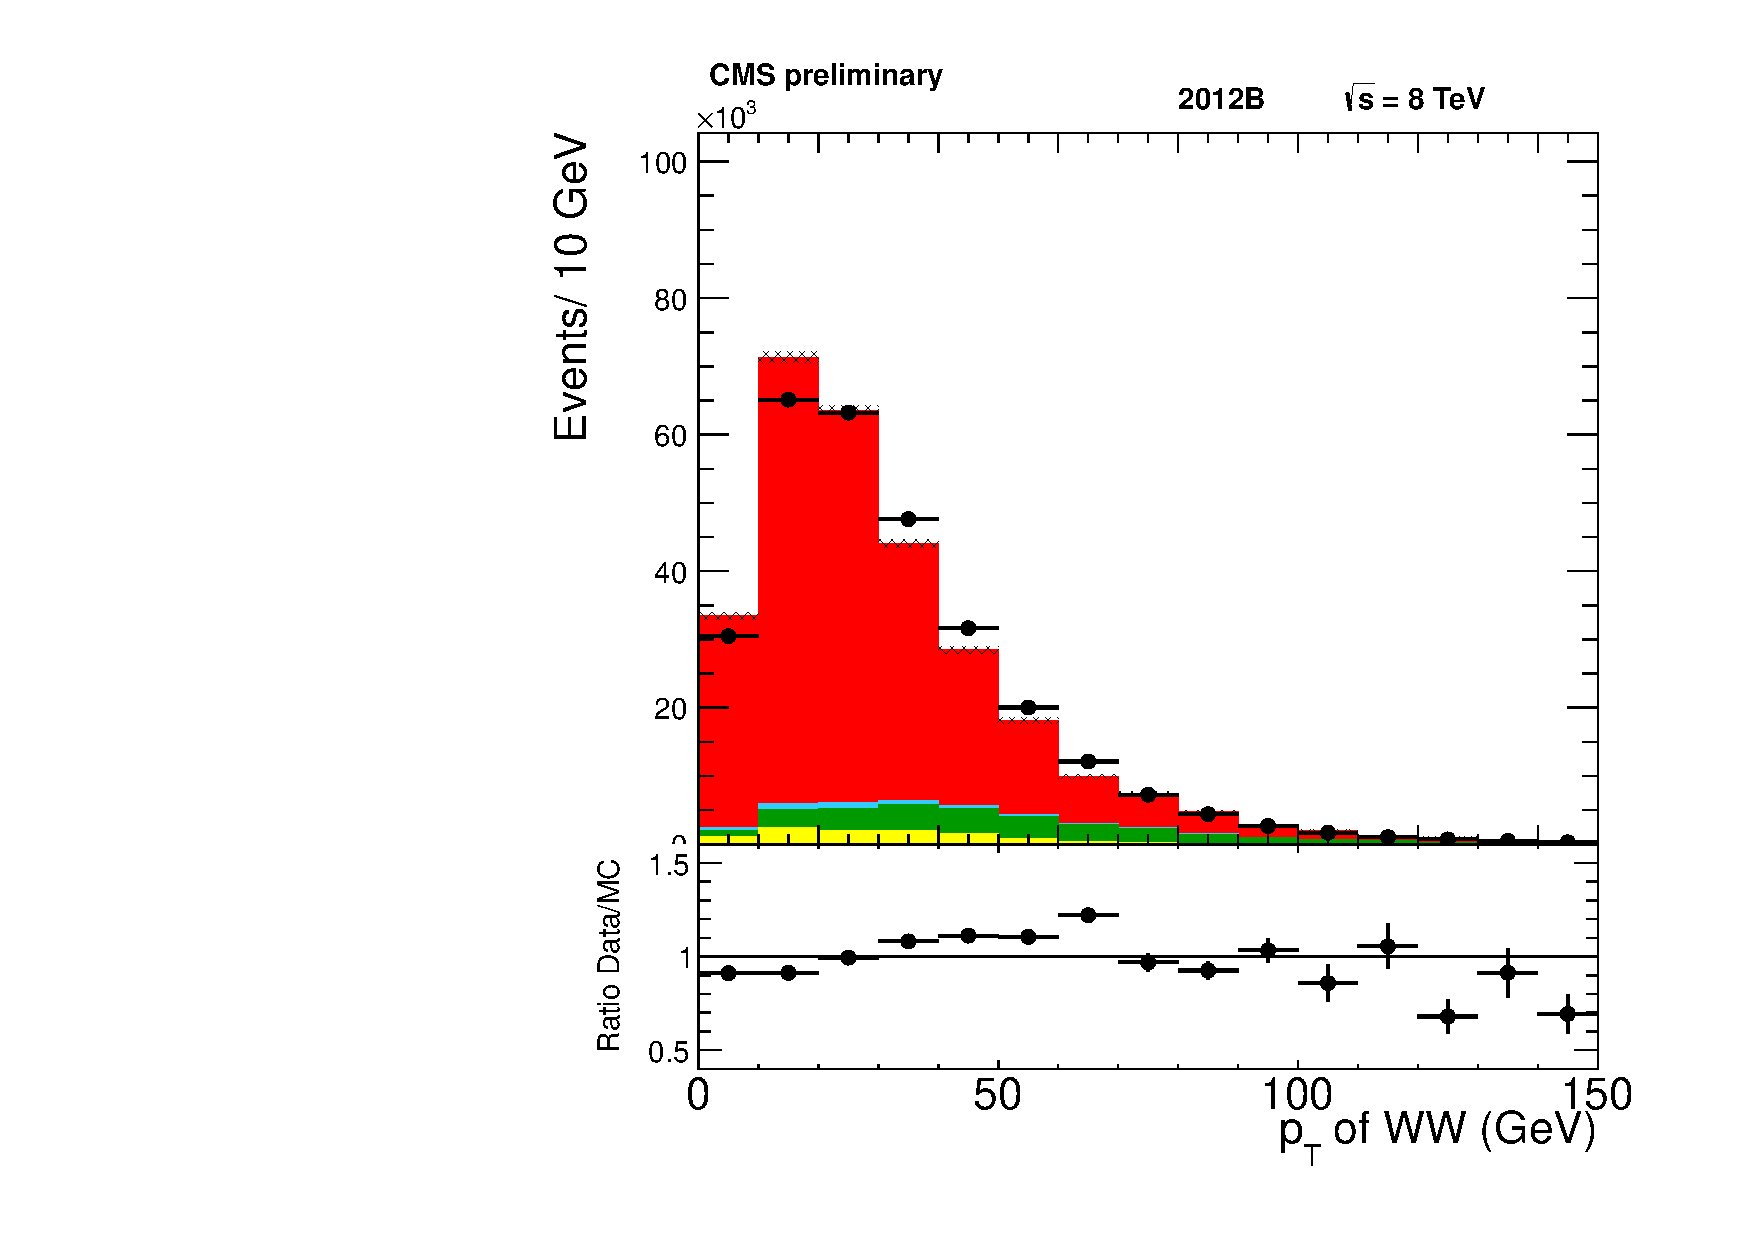
\includegraphics[width=0.4\textwidth]{plots/mu_ptlvjj_2012B.pdf}
    }
    \\
    \subfigure[2012A: WW $\eta$]{
      \includegraphics[width=0.4\textwidth]{plots/mu_etalvjj_2012A.pdf}
    }
    \subfigure[2012B: WW $\eta$]{
      \includegraphics[width=0.4\textwidth]{plots/mu_etalvjj_2012B.pdf}
    }
    \\
    \caption{ Comparison of the $p_{T}$ and  $\eta$ of the WW system from data and MC for the muon+jets selection.
            }
    \label{fig:CP2012AB9}
\end{figure}



\begin{figure}[htb]
  \centering
    \subfigure[2012A: $\cos\theta_{1}$]{
      \includegraphics[width=0.4\textwidth]{plots/el_ha_2012A.pdf}
    }
    \subfigure[2012B: $\cos\theta_{1}$]{
      \includegraphics[width=0.4\textwidth]{plots/el_ha_2012B.pdf}
    }
    \\
    \subfigure[2012A: $\cos\theta_{2}$]{
      \includegraphics[width=0.4\textwidth]{plots/el_hb_2012A.pdf}
    }
    \subfigure[2012B: $\cos\theta_{2}$]{
      \includegraphics[width=0.4\textwidth]{plots/el_hb_2012B.pdf}
    }
    \\
    \subfigure[2012A: $\cos\theta^{\ast}$]{
      \includegraphics[width=0.4\textwidth]{plots/el_hs_2012A.pdf}
    }
    \subfigure[2012B: $\cos\theta^{\ast}$]{
      \includegraphics[width=0.4\textwidth]{plots/el_hs_2012B.pdf}
    }
    \\
    \caption{ Comparison of the angular distributions for $\cos\theta_{1}$,$\cos\theta_{2}$ and $\cos\theta^{\ast}$ from data and MC for 
the electron+jets selection.
            }
    \label{fig:CP2012AB10}
\end{figure}

\begin{figure}[htb]
  \centering
    \subfigure[2012A: $\Phi$]{
      \includegraphics[width=0.4\textwidth]{plots/el_phi_2012A.pdf}
    }
    \subfigure[2012B: $\Phi$]{
      \includegraphics[width=0.4\textwidth]{plots/el_phi_2012B.pdf}
    }
    \\
    \subfigure[2012A: $\Phi_{1}$]{
      \includegraphics[width=0.4\textwidth]{plots/el_phib_2012A.pdf}
    }
    \subfigure[2012B: $\Phi_{1}$]{
      \includegraphics[width=0.4\textwidth]{plots/el_phib_2012B.pdf}
    }
    \\
    \subfigure[2012A: electron charge]{
      \includegraphics[width=0.4\textwidth]{plots/el_charge_2012A.pdf}
    }
    \subfigure[2012B: electron charge]{
      \includegraphics[width=0.4\textwidth]{plots/el_charge_2012B.pdf}
    }
    \\
    \caption{ Comparison of the angular distributions for $\Phi$ , $\Phi_{1}$ and electron charge from data and MC for
the electron+jets selection.
            }
    \label{fig:CP2012AB11}
\end{figure}

\begin{figure}[htb]
  \centering
    \subfigure[2012A: WW $p_{T}$]{
      \includegraphics[width=0.4\textwidth]{plots/el_ptlvjj_2012A.pdf}
    }
    \subfigure[2012B: WW $p_{T}$]{
      \includegraphics[width=0.4\textwidth]{plots/el_ptlvjj_2012B.pdf}
    }
    \\
    \subfigure[2012A: WW $\eta$]{
      \includegraphics[width=0.4\textwidth]{plots/el_etalvjj_2012A.pdf}
    }
    \subfigure[2012B: WW $\eta$]{
      \includegraphics[width=0.4\textwidth]{plots/el_etalvjj_2012B.pdf}
    }
    \\
    \caption{ Comparison of the $p_{T}$ and  $\eta$ of the WW system from data and MC for the muon+jets selection.
            }
    \label{fig:CP2012AB12}
\end{figure}


\begin{figure}[htb]
  \centering
    \subfigure[2012A: muon $m_{lvjj}$]{
      \includegraphics[width=0.4\textwidth]{plots/mu_mlvjj_2012A.pdf}
    }
    \subfigure[2012B: muon $m_{lvjj}$]{
      \includegraphics[width=0.4\textwidth]{plots/mu_mlvjj_2012B.pdf}
    }
    \\
    \subfigure[2012A: electron $m_{lvjj}$]{
      \includegraphics[width=0.4\textwidth]{plots/el_mlvjj_2012A.pdf}
    }
    \subfigure[2012B: electron $m_{lvjj}$]{
      \includegraphics[width=0.4\textwidth]{plots/el_mlvjj_2012B.pdf}
    }
    \\
    \caption{ Comparison of the four-body invariant mass from data and MC for the muon+jets selection (top)
             and electron+jets selection (bottom) .
            }
    \label{fig:CP2012AB13}
\end{figure}


